\documentclass[11pt, letterpaper]{article}
\usepackage[table]{xcolor}
\usepackage{graphicx} % Required for inserting images
\usepackage{titlesec}
\usepackage{float}
\usepackage{amsmath}
\usepackage{layout}
\usepackage{anyfontsize}
\usepackage{listings}
\usepackage{xcolor}
\usepackage{booktabs}
\usepackage{pdflscape}
\usepackage{lscape}
\usepackage{tabularx}
\usepackage{boldline}
\usepackage{tabulary}
\usepackage{tcolorbox}
\usepackage{hyperref}
\usepackage{amssymb} % Añadido para simbolos extra
\usepackage{changepage}

\usepackage[spanish,es-noindentfirst]{babel}
\usepackage[left=2.5cm, right=2.5cm, top=2.5cm, bottom=2.5cm]{geometry}
\usepackage[skip=5pt plus1pt, indent=20pt]{parskip}

\begin{document}

\begin{titlepage}
    \centering
    {\Huge \textsc{\textbf{}}\par}
    \par\vspace{1cm}
    % Asegúrate de tener el archivo de imagen o comenta la línea si no lo tienes
    \begin{figure}[H]
    \begin{minipage}{0.15\textwidth}
        \centering
        
\includegraphics[width=\textwidth]{imagenes/Logo_UPC.svg.png}
    \end{minipage}
    \hspace{0.02\textwidth}
    \begin{minipage}{0.85\textwidth}
        \centering
        
\includegraphics[width=\textwidth]{imagenes/logo-fiblletres-upc-color.png}
    \end{minipage}
    \end{figure}
    
    
    {\Huge \textsc{\textbf{}}\par}
    \vspace{2cm}
    {\huge \textbf{S{\LARGE ISTEMA} I{\LARGE NTELIGENTE} {\LARGE DE} A{\LARGE SISTENCIA} {\LARGE AL} D{\LARGE ESARROLLO} E{\LARGE STRUCTURADO} {\LARGE Y} S{\LARGE EGUIMIENTO} {\LARGE DE} P{\LARGE ROYECTOS} {\LARGE DE} S{\LARGE OFTWARE}}\par}
    \vspace{2cm}
    
    {\normalsize \Large\textbf{ {Adrià Cebrián Ruiz}}\\ \par}

    \vspace{2cm}
    {\normalsize \textbf{Director:} {Luis Jonás Cuervo Derqui (Colbai Advisors SL)}\par}
    %\vspace{0.2cm}
    {\normalsize \textbf{Ponente:} {David García Soriano (Departamento de Ciencias de la Computación)}\par}
    %\vspace{0.2cm}
    {\normalsize \textbf{Titulación:} {Grado en Ingeniería Informática (Computación)}\par}
    
    \vspace{1.5cm}
    
    {\normalsize \textbf{Memoria del trabajo de fin de grado}}\par
    {\normalsize\textbf{Facultat Informàtica de Barcelona (FIB)}}\par
    {\normalsize \textbf{Universitat Politècnica de Catalunya (UPC) - BarcelonaTech} \par}
    {\normalsize \textbf{\today}}
    \vfill
\end{titlepage}

\newpage

\begin{adjustwidth}{2cm}{2cm}
{ %Abstract inglees
\hspace{0pt} 
\vfill
\large
\begin{center}
{\textbf{Abstract}}
\end{center}
The present project consists of the design and application of an intelligent assistance system, with the objective of automating the various stages in the development of software projects ---requirements gathering, Spec-Driven Development, and client follow-up--- through the orchestration of generative Artificial Intelligence tools. Placing emphasis on the interaction with the human developer, following a philosophy of \textit{Human in the loop}, and the generation of documentation to guide the process. This methodology aims to reduce the quality loss typically caused by the use of AI in the development of these projects. The experimental evaluation conducted suggests improvements in code quality and maintainability when using the proposed system. This final degree project is applied and developed for the working environment at the software consulting company \textit{Colb.AI}.
\vfill
\hspace{0pt}
}

\newpage
{ %Abstract castellano
\hspace{0pt}
\vfill
\large 
\begin{center}
{\textbf{Resumen}}
\end{center}
El presente proyecto consiste en el diseño y aplicación de un sistema para la automatización de las diversas etapas en el desarrollo de proyectos de \textit{software} ---toma de requerimientos, \textit{Spec-Driven Development} y seguimiento del cliente--- utilizando principalmente la orquestación de herramientas de Inteligencia Artificial generativa. Haciendo un especial énfasis en la interacción de estos sistemas de automatización con el desarrollador, siguiendo una filosofía de \textit{Human in the loop}, y la generación de documentación para guiar el proceso. Esta metodología busca reducir la pérdida de calidad típicamente resultante del uso de IA en el desarrollo de los proyectos. La evaluación experimental realizada sugiere mejoras en la calidad y mantenibilidad del código al utilizar el sistema propuesto. Este trabajo de final de grado se aplica y desarrolla para el entorno laboral de la consultora de \textit{software} \textit{Colb.AI}.
\vfill
\hspace{0pt}
}
\newpage

{ %Abstract català
\hspace{0pt}
\vfill
\large
\begin{center}
{\textbf{Resum}}
\end{center}
El present projecte consisteix en el disseny i aplicació d'un sistema intel·ligent per a l'automatització de les etapes en el desenvolupament de projectes de \textit{software} ---toma de requeriments, \textit{Spec-Driven Development} i seguiment del client--- aplicant principalment l'orquestació d'eines d'Intel·ligència Artificial generativa. Es fa un especial èmfasi en la interacció d'aquests sistemes amb el desenvolupador humà, seguint una filosofia de \textit{Human in the loop}, i la generació de documentació per a guiar el procés. Aquesta metodologia tracta de reduir la pèrdua de qualitat típicament conseqüència de l'ús de la IA en el desenvolupament d'aquests projectes. L'avaluació experimental realitzada suggereix millores en la qualitat i mantenibilitat del codi utilitzant el sistema proposat. Aquest treball de final de grau s'aplica i desenvolupa per a l'entorn laboral de la consultoria de \textit{software} \textit{Colb.AI}.
\vfill
\hspace{0pt}
}
\end{adjustwidth}

\newpage
\tableofcontents
\newpage
\listoffigures
\listoftables
\newpage

\section{Introducción y contexto}
\label{sec:contexto}

El presente trabajo consiste en el diseño de un sistema de automatización para el desarrollo y diseño de proyectos de software, utilizando como pilar principal herramientas basadas en \textit{LLMs}. El desarrollo de este sistema se enmarca y diseña para su uso dentro de una empresa real, \textit{Colb.ai}, dedicada principalmente a la consultoría de proyectos de software.

Es innegable que las herramientas de inteligencia artificial, principalmente los \textit{Large Language Models}, están cambiando la forma en que se desarrollan los proyectos de software para la mayor parte de empresas del sector. Estas tecnologías presentan la oportunidad de automatizar muchas de las tareas que tradicionalmente habían sido llevadas a cabo exclusivamente por los desarrolladores humanos, pero su adopción sin la supervisión humana adecuada conlleva riesgos que pueden comprometer la calidad y sostenibilidad del software generado, sobre todo a largo plazo.

Se presentan a continuación tres módulos que se van a automatizar en el desarrollo de este TFG:
\begin{enumerate}
    \item \textbf{Toma de requerimientos y diseño de arquitectura:} Necesidades del cliente, exploración de \textit{frameworks} posibles a utilizar, y diseño de la arquitectura del proyecto.
    \item \textbf{Desarrollo del código:} Asistencia de programación al desarrollador, generación de código a partir de las especificaciones. Evitando la generación de código de baja calidad, principalmente mediante la generación de documentación y especificaciones previas a la generación de código.
    \item \textbf{Seguimiento del cliente:} Generación de informes de seguimiento para el cliente, basado en las reuniones con el mismo.
\end{enumerate}

\subsection{Definición del Problema}
\label{sec:definicion_problema}

El reto central de la automatización de estas tareas sin perder calidad, es conseguir un equilibrio entre la agilidad que ofrecen los asistentes de inteligencia artificial y la involucración de un desarrollador que garantice que cada paso cubre unos estándares de estructura y calidad. Este equilibrio es difícil de mantener en la práctica, y su dificultad puede explicarse a través de un principio en el ámbito de la psicología cognitiva: \textit{The Law of Least Effort}, o en otras palabras, la ley del mínimo esfuerzo. Esta teoría sostiene que los humanos y otros organismos tienden a priorizar la opción que presenta la menor resistencia para alcanzar sus objetivos, ya sea en términos de esfuerzo físico o cognitivo\cite{avoidance_of_cognitive_demand}. Aunque pueda parecer paradójico ---puesto que a las personas también nos gustan los retos y los puzles---\cite{inzlicht_effort_paradox_2018}, este fenómeno presenta una posible explicación al reto principal de la automatización, y es que el desarrollador tiene la tentación de delegar todo el trabajo en el asistente de IA sin involucrarse lo suficiente, comprometiendo así los estándares de calidad y estructura necesarios para poder elaborar un proyecto profesional y sostenible a largo plazo.

A continuación, se hace una definición mas especifica de los problemas y puntos a cubrir detectados en cada apartado de el proyecto.
\newpage 

\subsubsection{Toma de requerimientos y planificación de la arquitectura}
\label{sec:ProblemaTomaRequerimientos}

La toma de requerimientos es una fase especialmente crítica en el desarrollo de software, puesto que sienta las bases del proyecto: su alcance, las tecnologías a utilizar y la arquitectura del sistema. Si esta fase no se lleva a cabo con el adecuado rigor, puede suponer todo tipo de imprevistos en la etapa de desarrollo del proyecto, causando retrasos en la entrega del proyecto, incrementos en el presupuesto y, en ocasiones, dejando inservibles módulos ya implementados. 

Por lo tanto, es crucial que este apartado se lleve a cabo con la máxima calidad y supervisión humana posible, por lo que la automatización de este módulo deberá tener un componente importante de interacción con el diseñador.

\subsubsection{Desarrollo de código}
\label{sec:ProblemaDesarrolloCodigo}

Actualmente, los asistentes de código más populares (GitHub Copilot, Cursor, Claude Code, etc.) operan bajo un paradigma \textit{Code-Driven}: el desarrollador describe vagamente lo que quiere y el modelo genera código de forma inmediata, sin exigir ninguna especificación previa. Este enfoque tiene tres consecuencias negativas directas:

\begin{itemize}
    \item \textbf{Generación de \textit{slop code}:} El código producido resuelve el problema inmediato, pero carece de estructura coherente, no sigue los estándares del proyecto y acumula deuda técnica. Al no haber una especificación de referencia, el modelo no puede saber qué es correcto más allá de lo que el usuario describe en ese momento. El resultado es un código difícil de mantener, escalar o auditar.

    \item \textbf{Falta de trazabilidad entre requisitos y código:} Sin un documento de especificación que actúe como fuente de verdad, resulta imposible saber si el código generado cumple realmente con los requisitos del negocio, si ha habido desviaciones respecto al diseño original, o quién tomó qué decisión y cuándo.

    \item \textbf{Barrera de incorporación para nuevos desarrolladores:} La ausencia de documentación estructurada convierte la incorporación de un nuevo miembro al equipo en un proceso lento y costoso. Sin especificaciones claras que expliquen el \textit{porqué} de cada decisión de diseño, el nuevo desarrollador debe deducir la arquitectura y las reglas del proyecto leyendo directamente el código, lo que ralentiza su productividad y aumenta el riesgo de que introduzca cambios inconsistentes con la visión original del sistema.
\end{itemize}

Por otro lado, las herramientas que sí exigen especificación previa (como Spec Kit o AgentOS) presentan el problema opuesto: generan una fricción operativa excesiva, produciendo documentación desproporcionada incluso para cambios pequeños, lo que las hace incompatibles con metodologías ágiles reales.

\subsubsection{Seguimiento del cliente}
\label{sec:ProblemaSeguimientoCliente}

Este apartado se considera considerablemente relevante en el ámbito de la consultoría, debido a que la relación y el involucramiento con el cliente son un componente esencial para que un proyecto de software progrese adecuadamente. En la empresa \textit{Colb.AI} se acostumbra a escribir un documento \textit{Word} de seguimiento para el cliente después de cada reunión de seguimiento, para dejarle al cliente por escrito los temas tratados en la reunión, con las tareas cubiertas, las pendientes por cubrir, y el estado actual de la implementación.

\subsection{Conceptos Relevantes Previos}
\label{sec:conceptos_relevantes}
Los principales conceptos y definiciones relevantes que envuelven los ámbitos tratados en este TFG son los siguientes:

\subsubsection{Spec-Driven-Development (SDD)}
\label{sec:sdd}

El \textit{Spec-Driven Development} (SDD) es una filosofía donde la documentación detallada de los requisitos y el comportamiento esperado del sistema (la especificación) dirige la creación del software. A diferencia del enfoque tradicional, donde estos documentos descriptivos solían quedar subordinados o desactualizarse frente al código, el SDD invierte esta relación. El documento estructurado en lenguaje natural actúa como la base de la verdad sobre la que se construirá el futuro código. \cite{ostroff_agile_2004} \cite{github_spec_kit}

En otras palabras, hay que tener definido previamente exactamente qué queremos que haga cada pieza de código, y cómo queremos que lo haga. Cuando se quiera hacer cambios en la implementación, se han de aplicar primero en los documentos de especificación y luego en el código del proyecto. \\

\subsubsection{Toma de requerimientos}
\label{sec:toma_requerimientos}

La toma de requerimientos (en inglés \textit{Requirements Gathering}) es una fase fundamental dentro de la ingeniería de software. En ella se investigan, descubren y extraen las necesidades de los clientes, usuarios y otras partes interesadas del sistema. A través de conversaciones con un cliente, que en muchas ocasiones no está muy seguro de qué quiere exactamente, el analista debe generar diseños y especificaciones funcionales específicas con comportamientos detallados \cite{jama_requirements} \cite{sommerville_se_2015}.

\subsubsection{Asistentes de Inteligencia Artificial y Agentes Basados en LLMs}
\label{sec:asistentes_ia}

En el ámbito del desarrollo de software, los Modelos de Lenguaje de Gran Tamaño (LLMs) son la base tecnológica tanto de los asistentes de código como de los sistemas de procesamiento de documentos. Un asistente basado en LLM actúa como un colaborador interactivo que puede ayudar al desarrollador a generar código, pero también a analizar transcripciones de reuniones, estructurar requerimientos o redactar documentación de seguimiento. Para comprender cómo estas herramientas se estructuran y evolucionan en este proyecto, es necesario definir los siguientes conceptos clave:

\begin{itemize}
    \item \textbf{Instrucciones (\textit{Prompts}):} Son las entradas en lenguaje natural que el usuario utiliza para comunicarse con el modelo. Un \textit{prompt} define la tarea a realizar y proporciona el contexto y las restricciones necesarias.

    \item \textbf{Agentes de Código:} Un agente es un asistente al que se le asigna un rol mediante un \textit{prompt} y se le equipa con distintas \textit{Agent Skills} y herramientas varias. Su propósito es llevar a cabo una tarea específica. Además, es posible encadenar varios agentes especializados para construir un sistema coordinado. \cite{vscode_agents} \cite{wang_llm_agents_2024}

    \item \textbf{Habilidades del Agente (\textit{Agent Skills}):} Son funciones, herramientas o \textit{scripts} específicos que el agente puede invocar para ejecutar acciones tangibles sobre el entorno local, como leer, crear o modificar archivos en un repositorio. \cite{agentskills_home} \cite{yao_react_2023}
\end{itemize}

\subsubsection{Transcripción automática y diarización}
\label{sec:transcripcion_diarizacion}

La transcripción automática es el proceso de convertir el audio de una conversación en texto estructurado mediante modelos de reconocimiento de voz. Un concepto clave asociado es la \textit{diarización} (\textit{speaker diarization}): la capacidad de identificar y etiquetar qué fragmento de texto fue pronunciado por cada hablante. En el contexto de la toma de requerimientos, esta atribución resulta especialmente relevante, ya que permite distinguir qué peticiones o restricciones provienen del cliente y cuáles son comentarios del equipo técnico, mejorando así la calidad de la especificación resultante. \cite{radford2022whisper}

\subsection{Stakeholders}
\label{sec:stakeholders}

Los principales stakeholders implicados en esta situación son los siguientes:

\subsubsection{Desarrolladores}
\label{sec:desarrolladores}

Los primeros beneficiarios de la implantación de este sistema son los desarrolladores y diseñadores de software. Al implementar metodologías de código orientadas a la creación de código estructurado y documentado, el mantenimiento del código se haría mucho más sencillo, así como el desarrollo y entendimiento de este. Modularizando las distintas \textit{features} e implementaciones de código, facilitaríamos el entendimiento de la estructura general del producto, lo cual resultaría altamente beneficioso para su futura escalabilidad y mantenimiento. Además, el módulo de toma de requerimientos les proporciona las especificaciones ya estructuradas antes de comenzar el desarrollo, reduciendo la ambigüedad y el tiempo invertido en interpretar notas informales de reuniones.

\subsubsection{Consultores}
\label{sec:consultores}

Los consultores son los miembros del equipo responsables de gestionar la relación con el cliente y coordinar el avance del proyecto. Son los principales beneficiarios de los módulos de toma de requerimientos y seguimiento del cliente: actualmente invierten un tiempo considerable en estructurar manualmente las necesidades expresadas por el cliente en conversaciones informales y en redactar la documentación de seguimiento posterior a cada reunión. La automatización de estas tareas les permite centrarse en el trabajo de mayor valor añadido: el análisis, la toma de decisiones y la relación directa con el cliente.

\subsubsection{Cliente y sus usuarios}
\label{sec:cliente_usuarios}

Tener un código bien estructurado y entendido en profundidad por sus creadores significa un producto de mayor calidad, más fácil de mantener y, en muchos casos, más seguro y eficiente. Además, el cliente se beneficia directamente del módulo de seguimiento: recibe documentación estructurada y consistente tras cada reunión, con los acuerdos alcanzados y los próximos pasos claramente definidos para ambas partes, sin la latencia habitual en la producción manual de este tipo de documentación.


\subsection{Estado del arte y soluciones existentes}
\label{sec:estado_arte}
Para contextualizar el desarrollo de nuestro sistema, es fundamental analizar las herramientas actuales que buscan resolver problemas similares en el ámbito de la ingeniería de software asistida por IA.

\subsubsection{Spec Kit}
\label{sec:spec_kit}
Spec Kit es una herramienta diseñada específicamente para facilitar el desarrollo basado en especificaciones. Su enfoque principal radica en la generación de documentos de diseño y arquitectura como paso previo y obligatorio a la implementación de código, estructurando así el ciclo de vida del desarrollo. \cite{github_spec_kit}

\subsubsection{AgentOS}
\label{sec:agentos}
AgentOS propone un marco de trabajo (\textit{framework}) integral para la creación y orquestación de agentes autónomos. Proporciona una estructura robusta que permite a los desarrolladores construir sistemas basados en inteligencia artificial capaces de ejecutar tareas complejas y encadenadas de forma independiente. \cite{buildermethods_agent_os} \cite{yao_react_2023}

\subsubsection{Asistentes Comerciales (Copilot, Cursor)}
\label{sec:asistentes_comerciales}
En el mercado actual destacan diversas herramientas comerciales de asistencia a la programación impulsadas por IA, tales como GitHub Copilot, Cursor o Devin. Estas soluciones son altamente eficientes para la generación de código en tiempo real y la resolución de dudas técnicas, operando bajo un paradigma principalmente \textit{Code-Driven} (orientado a la escritura directa de código). \cite{github_copilot_docs} \cite{cursor_ai} \cite{chen_codex_2021} \cite{peng_copilot_2023}

\subsubsection{Herramientas de transcripción de reuniones}
\label{sec:herramientas_transcripcion}
La obtención de una transcripción como punto de partida es un requisito compartido por los módulos de toma de requerimientos y seguimiento del cliente. Las principales soluciones existentes se dividen en dos categorías según el tipo de reunión.

Para reuniones telemáticas, las plataformas de videoconferencia más extendidas (Microsoft Teams, Google Meet, Zoom) ofrecen transcripción automática integrada con diarización nativa, ya que cada participante habla desde su propio dispositivo. Para reuniones presenciales, las alternativas principales son Whisper \cite{radford2022whisper}, el modelo de reconocimiento de voz de OpenAI (ejecución local, sin coste de API, pero sin diarización nativa), y \textbf{Azure Speech Service} (servicio cloud con diarización de hablantes). Se optó por Azure Speech Service al estar incluido en la suscripción de Azure de Colb.AI y por ofrecer resultados satisfactorios en las pruebas realizadas.

\subsubsection{Herramientas de documentación de reuniones}
\label{sec:herramientas_documentacion_reuniones}
Existen herramientas comerciales orientadas a la generación automática de resúmenes y documentación post-reunión, como Otter.ai, Fireflies.ai o Microsoft Copilot for Teams. Estas soluciones se descartaron por dos razones complementarias: en primer lugar, generan resúmenes genéricos no parametrizables, sin posibilidad de adaptar el formato al tipo de reunión o al cliente concreto de Colb.AI; en segundo lugar, ya se disponía de ClaudeCode con skills, capaz de generar documentación de seguimiento con la misma eficacia a través de un skill dedicado. Por otro lado, la implementación de un módulo Python propio para este fin no supone una complejidad técnica elevada, lo que refuerza la decisión de desarrollar una solución a medida en lugar de depender de una herramienta externa.

\subsubsection{Asistentes CLI extensibles}
\label{sec:asistentes_cli}
Las herramientas de asistencia a la programación de tipo CLI (\textit{Command-Line Interface}) representan una categoría diferenciada de los asistentes integrados en el IDE. Operan directamente desde la terminal con acceso nativo al sistema de archivos y exponen mecanismos de extensibilidad nativos ---plugins, hooks de ciclo de vida y el protocolo MCP (\textit{Model Context Protocol})--- que permiten definir flujos de trabajo de programación estructurados de forma composable. Las dos principales herramientas de este tipo son ClaudeCode \cite{claude_code_2024} (Anthropic) y OpenCode \cite{opencode_2025} (open source, compatible con modelos locales y remotos).

\subsubsection{superpowers plugin}
\label{sec:superpowers}
\textit{superpowers} es un plugin open source para ClaudeCode que implementa el patrón orquestador + subagentes mediante skills. Proporciona una arquitectura base para flujos de trabajo \textit{Spec-First}, en la que un agente orquestador coordina subagentes especializados a través de skills reutilizables. Sin embargo, carece de un mecanismo de constitución ni de features compartidas entre sesiones o desarrolladores distintos, lo que limita su capacidad para garantizar coherencia arquitectónica a lo largo del ciclo de vida de un proyecto.

\subsection{Análisis comparativo: ¿Está justificada una solución a medida?}
\label{sec:analisis_comparativo}

Si bien las alternativas mencionadas presentan avances significativos, su aplicación directa en nuestro entorno de trabajo plantea diversos desafíos operativos y arquitectónicos. 

En primer lugar, los asistentes puramente comerciales fomentan un ciclo de desarrollo directo e impulsivo. Al no exigir una especificación estructurada previa, agravan el problema del \textit{slop code} (código descuidado o de baja calidad estructural) mencionado en la introducción. Por otro lado, herramientas enfocadas en la especificación como Spec Kit generan una fricción operativa excesiva, produciendo una cantidad desproporcionada de documentos incluso para implementar \textit{features} muy sencillas, lo que ralentiza el desarrollo ágil. Finalmente, marcos de trabajo como AgentOS están diseñados bajo un enfoque \textit{greenfield} (proyectos creados desde cero), resultando sumamente complejos de integrar en repositorios \textit{legacy} o ya existentes.

En el Cuadro \ref{tab:comparativa_herramientas} se presenta un resumen de las características y limitaciones que estas soluciones presentan:

% Nota: Asegúrate de tener \usepackage{booktabs} en tu preámbulo para que esta tabla se renderice correctamente.
\begin{table}[H]
\centering
\begin{tabularx}{\textwidth}{>{\raggedright\arraybackslash}X >{\raggedright\arraybackslash}X >{\raggedright\arraybackslash}X >{\raggedright\arraybackslash}X}
    \toprule
    \textbf{Herramienta} & \textbf{Enfoque Principal} & \textbf{Inconveniente Principal} & \textbf{Integración en Código Existente} \\
    \midrule
    \textbf{Spec Kit} & Basado en especificaciones & Exceso de documentación, alta fricción operativa & Moderada \\
    \textbf{AgentOS} & Orquestación de agentes & Diseñado principalmente para proyectos \textit{greenfield} & Muy compleja (\textit{Legacy}) \\
    \textbf{Copilot/Cursor} & \textit{Code-Driven} & Fomenta el \textit{slop code}, falta de planificación & Alta (pero sin contexto global) \\
    \textbf{ClaudeCode / OpenCode} & CLI extensible mediante plugins y MCP & Requiere plugin/configuración para imponer flujo \textit{Spec-First} & Alta \\
    \textbf{superpowers} & Orquestador + subagentes via skills & Sin constitución ni \textit{features} globales entre sesiones & Alta \\
    \bottomrule
\end{tabularx}
\caption{Comparativa de soluciones existentes. Elaboración propia.}
\label{tab:comparativa_herramientas}
\end{table}

De las herramientas analizadas, \textit{superpowers} fue evaluado como candidato directo al problema planteado. Resuelve la orquestación de agentes, pero no garantiza coherencia arquitectónica entre sesiones ni entre desarrolladores distintos, ya que carece de un mecanismo de contexto persistente y compartido. Se decidió adoptarlo como base y extenderlo: el resultado es \textbf{colbPowers}, que añade la capa de \texttt{constitution.md} (reglas y estándares del proyecto) y \texttt{features.md} (registro de funcionalidades) como fuente de verdad compartida para todos los agentes.

A la vista de estas limitaciones, la creación de una solución propia resulta razonable. Desarrollar nuestro propio sistema nos proporciona la flexibilidad indispensable para integrarlo de forma nativa con nuestro \textit{pipeline} de trabajo. Esto nos permitirá personalizar la ingesta de contexto conectando la herramienta directamente a nuestras bases de datos, permitiendo la lectura automatizada de \textit{issues en GitHub} y la integración fluida con plataformas de gestión interna como \textit{Odoo} y \textit{Microsoft Teams}.

\subsection{Propuesta de implementación}
\label{sec:propuesta_implementacion}

Concluido que las herramientas preexistentes no se adaptan plenamente a nuestros requerimientos de agilidad e integración, nuestra propuesta toma inspiración de sus puntos fuertes para construir un sistema a medida.

Aprovechando la arquitectura de \textit{superpowers}, el proyecto propone el desarrollo de \textbf{colbPowers}: un plugin para ClaudeCode y OpenCode que extiende el patrón orquestador/subagentes añadiendo una capa de contexto persistente basada en \texttt{constitution.md} y \texttt{features.md}. Este plugin estructura el ciclo de vida del software en torno a tres pilares complementarios:

\begin{enumerate}
    \item \textbf{Toma de requerimientos:} transformar transcripciones de reuniones en planes de implementación estructurados mediante búsqueda semántica web.
    \item \textbf{Spec-Driven Development:} garantizar que cada implementación esté precedida de una especificación validada, coordinada por un agente orquestador que invoca subagentes especializados (implementador, revisor de código, revisor de compatibilidad con specs/constitución/features).
    \item \textbf{Seguimiento del cliente:} automatizar la generación de documentación post-reunión con el formato específico de Colb.AI.
\end{enumerate}

Originalmente se contempló construir este sistema desde cero. Durante la fase de investigación previa (TP1) se descubrió que \textit{superpowers} ya ofrecía la arquitectura base necesaria, lo que permitió redirigir el esfuerzo hacia la contribución diferencial: la capa de constitución y features, y los tres pilares del ciclo de vida del software.

\subsection{Flujo de trabajo completo}
\label{sec:flujo_completo}

La Figura~\ref{fig:flujo_completo} muestra el flujo de trabajo del sistema de principio a fin. El proceso arranca con la \textbf{toma de requerimientos}: la primera reunión con el cliente se transcribe de forma diferente según su modalidad ---en reuniones telemáticas se aprovechan las transcripciones automáticas de plataformas como Teams o Meet, mientras que en reuniones presenciales se graba el audio y se procesa con Azure Speech Service con diarización de hablantes--- y el texto resultante alimenta el módulo de procesamiento, que puede ejecutarse mediante la \textit{skill} de Claude Cowork o mediante la implementación propia en Python con LangChain y Tavily. En ambos casos, la salida es un plan de implementación estructurado que el usuario revisa y aprueba antes de continuar.

A partir de ese plan aprobado, el flujo entra en la fase de \textbf{desarrollo con colbPowers}: el agente orquestador guía al equipo a través del ciclo SDD completo ---definición del contexto del proyecto, especificación de la funcionalidad, implementación y revisión---, con puntos de validación humana en cada etapa que garantizan el principio de \textit{Human in the Loop}.

Una vez entregado el desarrollo, el sistema no termina: comienza la fase de \textbf{seguimiento del cliente}. Al igual que en la toma de requerimientos, la transcripción de la reunión de seguimiento se obtiene de forma automática si es telemática, o mediante Azure Speech si es presencial. A partir de ella, Claude Cowork o la alternativa propia generan un documento Word con el resumen, las decisiones tomadas y los próximos pasos. Si en esa reunión se identifican nuevas funcionalidades, el flujo regresa directamente a colbPowers para iniciar un nuevo ciclo de desarrollo --- convirtiendo el sistema en un \textbf{bucle continuo} que acompaña al proyecto durante toda su vida útil.

\begin{figure}[H]
    \centering
    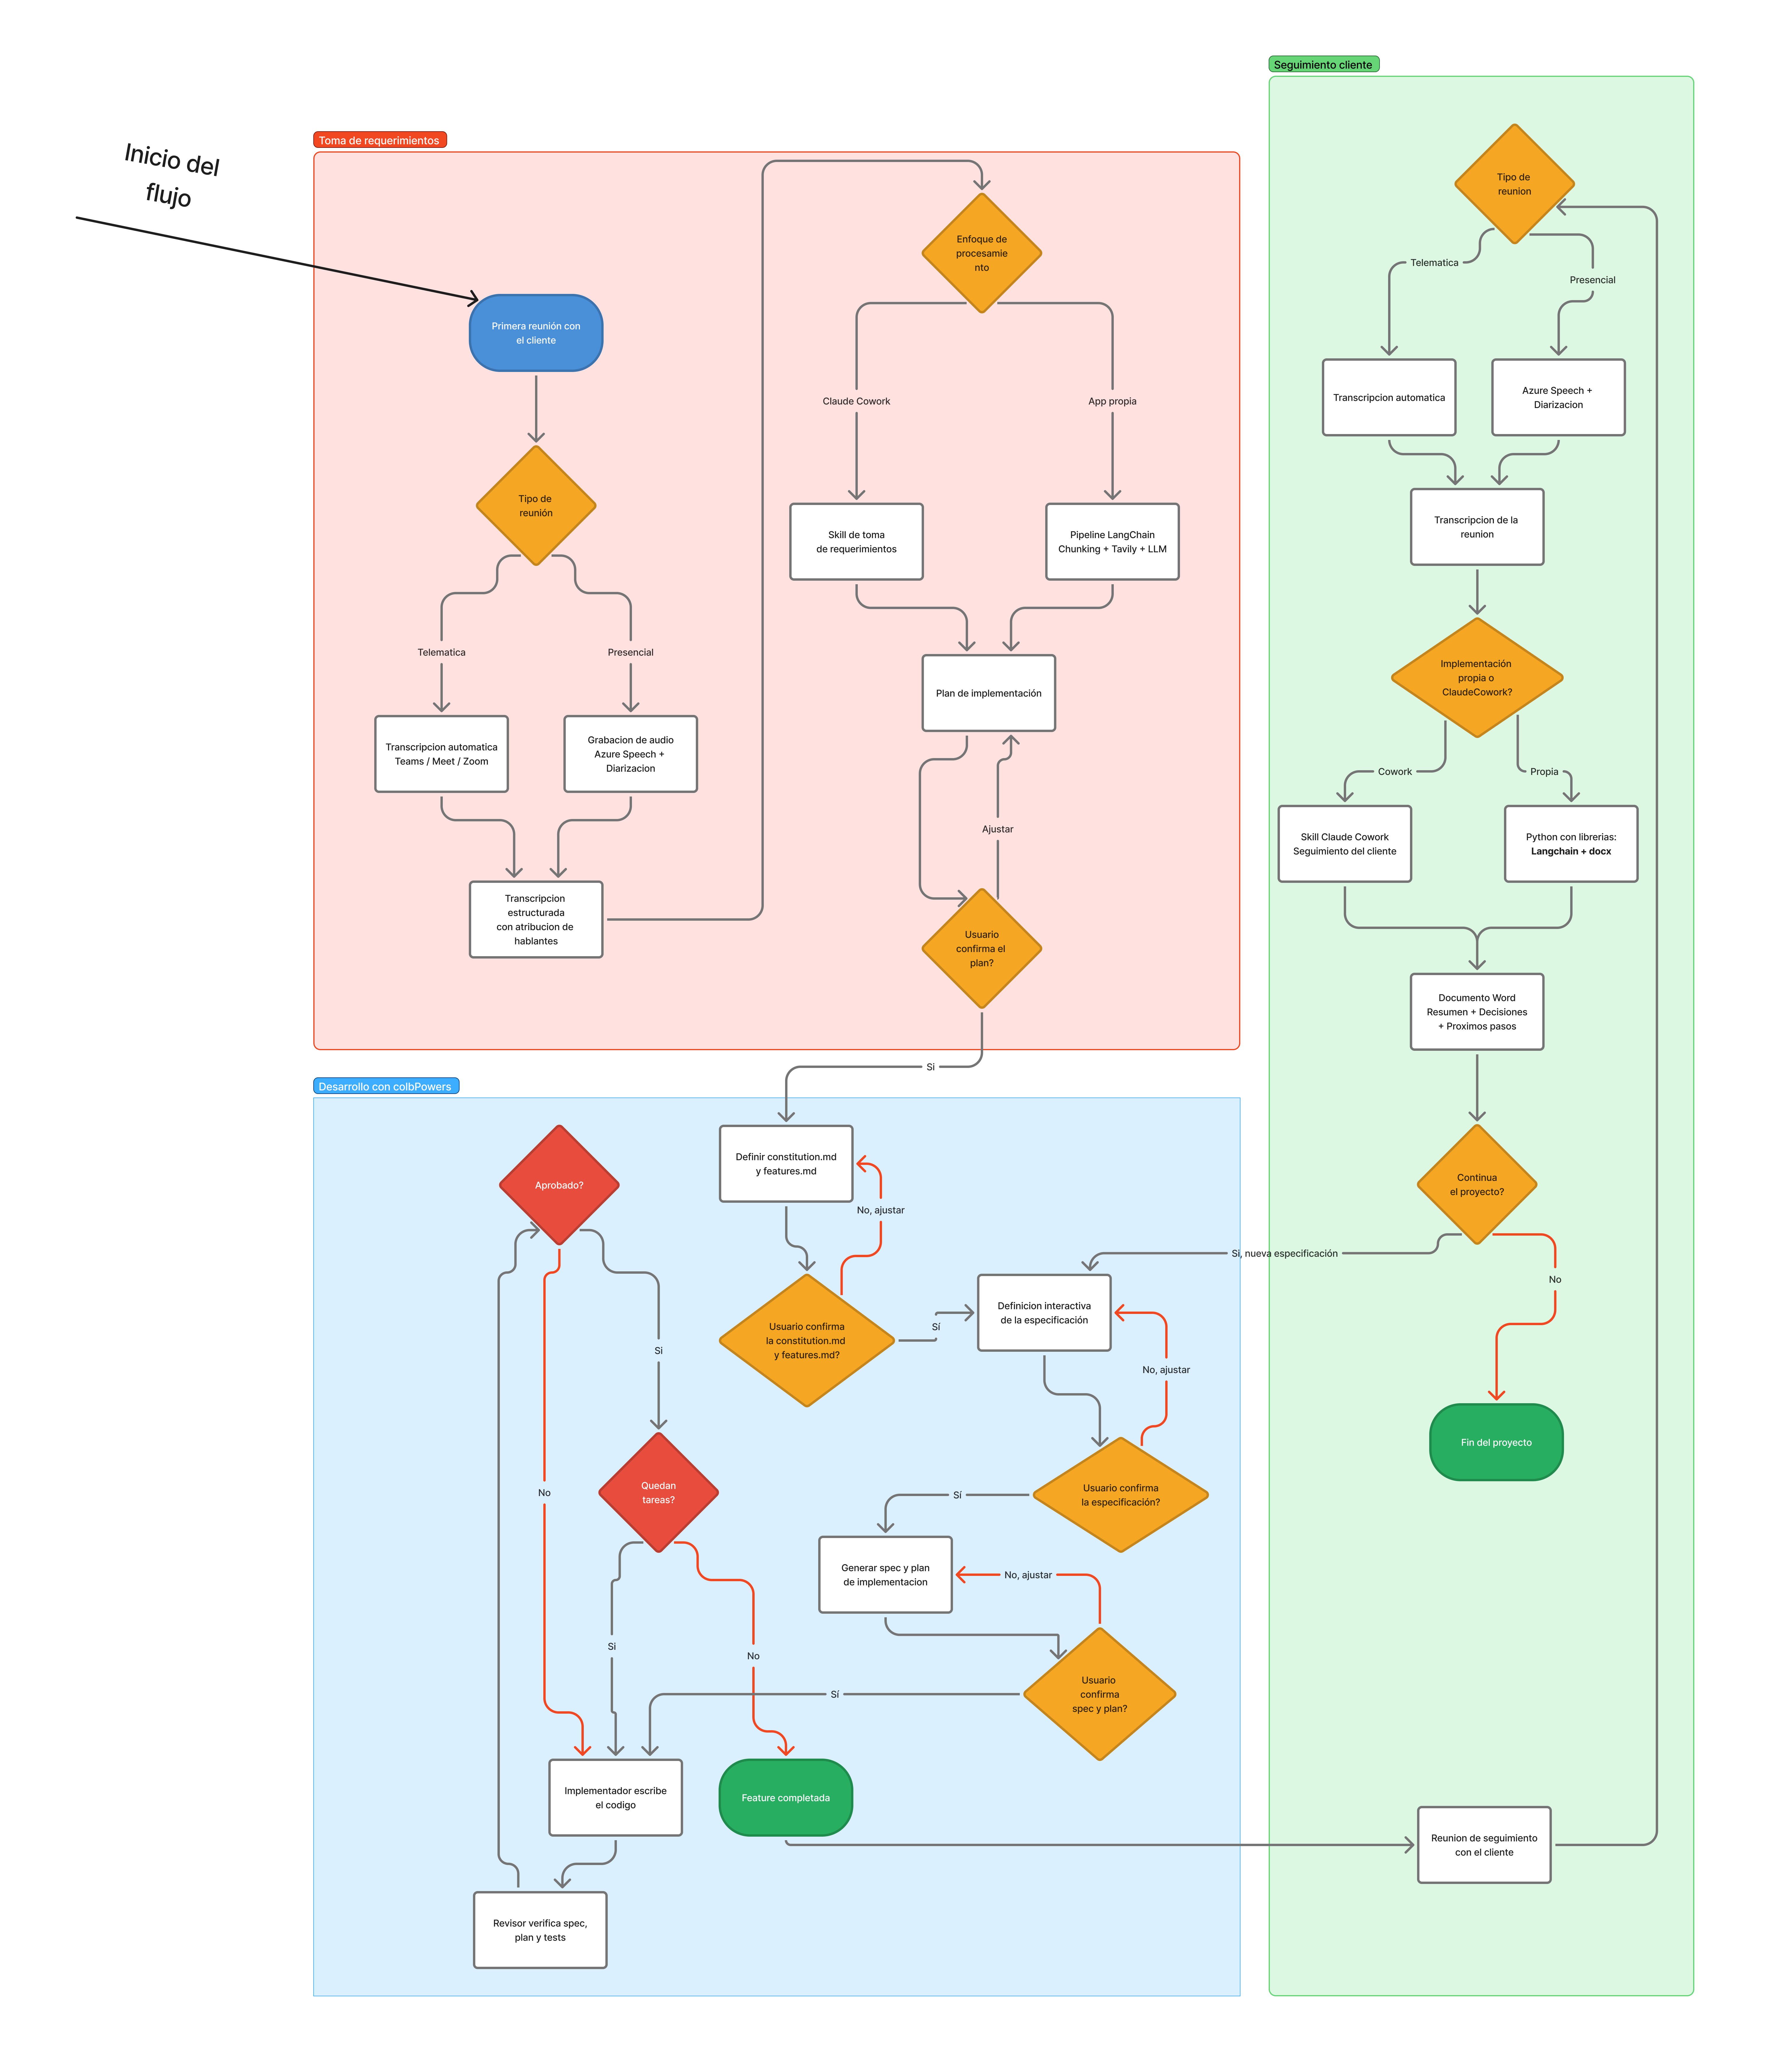
\includegraphics[width=\textwidth]{imagenes/DiagramaFlujoTrabajoCompleto.png}
    \caption{Flujo de trabajo completo del sistema: desde la primera reunión con el cliente hasta el seguimiento iterativo del proyecto.}
    \label{fig:flujo_completo}
\end{figure}

\newpage

\section{Alcance del Proyecto}
\label{sec:alcance}

De acuerdo con las necesidades de \textit{Colb.Ai} y la filosofía de documentar primero reglas y planes de implementación, este proyecto se centrará en el desarrollo de \textbf{colbPowers}: un plugin para los asistentes CLI ClaudeCode y OpenCode que extiende el patrón orquestador/subagentes de \textit{superpowers} añadiendo una capa de contexto persistente basada en \texttt{constitution.md} y \texttt{features.md}. Este plugin cubre el ciclo de vida completo de un proyecto software, desde la toma de requerimientos hasta el seguimiento del cliente, estructurando el desarrollo bajo la metodología \textit{Spec-Driven Development (SDD)}.

\subsection{Objetivo General}
\label{sec:objetivo_general}
El objetivo principal de este proyecto es diseñar e implementar un \textbf{sistema integral de asistencia al desarrollo de software}, articulado en tres pilares originales:

\begin{enumerate}
    \item \textbf{Plugin colbPowers} para los asistentes CLI ClaudeCode y OpenCode: extiende \textit{superpowers} añadiendo \texttt{constitution.md} y \texttt{features.md} como contexto persistente compartido entre sesiones y desarrolladores, e implementa el flujo \textit{Spec-First} mediante un agente orquestador y subagentes especializados. La integración con OpenCode requirió el análisis en profundidad de su arquitectura interna ---disponible como software libre--- y el desarrollo manual de \textit{hooks} nativos en JavaScript. Este trabajo fue necesario para lograr la compatibilidad de OpenCode con herramientas como \textit{code-review-graph}, que implementan su integración mediante hooks nativos de ClaudeCode: dado que los sistemas de hooks de ambos asistentes difieren arquitectónicamente, fue necesario implementar los adaptadores equivalentes en JavaScript para que OpenCode pudiera invocar estos servidores MCP con el mismo comportamiento.
    \item \textbf{Módulo de toma de requerimientos}: transforma transcripciones de reuniones con el cliente en planes de implementación estructurados. Incluye un componente de transcripción con Azure Speech Service (con diarización de hablantes y gestión idempotente mediante máquina de estados y hashes SHA-256) y un pipeline de procesamiento propio basado en LangChain y Tavily para búsqueda semántica y síntesis arquitectónica.
    \item \textbf{Módulo de seguimiento del cliente}: automatiza la generación de documentación post-reunión en el formato específico de Colb.AI, disponible como skill de Claude Cowork y como implementación propia de código abierto con python-docx.
\end{enumerate}

El conjunto opera de forma integrada en el entorno local del desarrollador, cubriendo el ciclo de vida completo del software desde la primera reunión con el cliente hasta la entrega y seguimiento iterativo del producto.

La validación de los resultados del sistema se hará a través de ciertas métricas de análisis de calidad del código, conocidas y utilizadas en el paradigma del desarrollo de software. Además de, por supuesto, los revisores humanos, que han de analizar en todo momento el código generado y los resultados producidos, haciendo a este un sistema con lo que se conoce \textit{Human In The Loop}, cosa que significa que en todo momento hay supervisión e intervención humana. \\

Para alcanzar el objetivo general, se establecen los siguientes sub-objetivos funcionales y arquitectónicos:
\begin{itemize}
    \item \textbf{Separación efectiva de responsabilidades en el ciclo de desarrollo:} Conseguir que cada fase del proceso (diseño, implementación y revisión) sea ejecutada con criterios y restricciones propios, garantizando que ninguna etapa sea omitida. Esta separación se materializa mediante skills que invocan subagentes especializados: un agente implementador, un agente revisor de código y un agente revisor de compatibilidad con las especificaciones, la constitución y las features del proyecto.

    \item \textbf{Coherencia arquitectónica mantenida a lo largo de todo el proyecto:} Lograr que los agentes dispongan en todo momento de un contexto actualizado con las reglas del proyecto, su \textit{roadmap} y el estado de las tareas, eliminando las inconsistencias causadas por la pérdida de memoria entre sesiones. Esta coherencia se implementa concretamente mediante \texttt{constitution.md} y \texttt{features.md} como fuente de verdad compartida entre sesiones y desarrolladores.

    \item \textbf{Agentes capaces de actuar de forma autónoma sobre el repositorio:} Obtener que los agentes puedan ejecutar acciones tangibles y verificables sobre el entorno local del proyecto —más allá de la mera generación de texto— convirtiéndolos en colaboradores activos capaces de materializar cambios reales en el código.

    \item \textbf{Trazabilidad completa entre especificación y código entregado:} Garantizar que cada funcionalidad implementada pueda rastrearse desde su especificación original hasta el código final revisado. Esta trazabilidad se garantiza porque todo cambio debe ser coherente con \texttt{constitution.md} y \texttt{features.md} antes de ser implementado, ofreciendo evidencia verificable de que lo entregado es coherente con lo planificado y cumple los estándares de calidad definidos.
\end{itemize}

\subsection{Requerimientos}
\label{sec:requerimientos}

\subsubsection{Requerimientos Funcionales}
\label{sec:req_funcionales}
\begin{itemize}
    \item El sistema debe permitir la ingesta y gestión de reglas fundamentales del proyecto (pila tecnológica, estándares de código) y mantener un registro actualizado de las características a desarrollar.
    \item El sistema debe ser capaz de interpretar funcionalidades de alto nivel y desglosarlas en un plan de tareas granulares y estructuradas.
    \item El sistema debe incluir un mecanismo de auditoría autónoma que contraste el código fuente generado con las especificaciones documentadas, para ver si existe algún conflicto con las documentación y el código generado.
    \item Se le ha de ofrecer al desarrollador métricas para analizar la calidad y la estructura del código generado. Las métricas utilizadas serán: \textit{Complejidad Ciclomática}\cite{McCabe_Complexity} del código, y el Índice de Sostenibilidad del Código \cite{microsoft_maintainability_index}.
    \item El sistema debe incluir un módulo de procesamiento de transcripciones capaz de generar planes de implementación estructurados a partir de reuniones con el cliente, explorando automáticamente los \textit{frameworks} y tecnologías relevantes mediante búsqueda semántica en la web.
    \item El sistema debe incluir un módulo de generación de documentación de seguimiento post-reunión con el formato específico de Colb.AI, a partir de la transcripción de reuniones periódicas con el cliente.
\end{itemize}

\subsubsection{Requerimientos No Funcionales}
\label{sec:req_no_funcionales}
\begin{itemize}
    \item \textbf{Transparencia y Trazabilidad:} Todo el estado, la memoria y las normativas manejadas por los agentes deben persistir en formatos de texto en un sistema de control de versiones.
    \item \textbf{Integración con asistentes CLI:} El plugin debe ser compatible con ClaudeCode y OpenCode, utilizando sus mecanismos nativos de extensibilidad (MCP, hooks, skills) para actuar directamente sobre los archivos locales del proyecto.
    \item \textbf{Modularidad:} El diseño de los roles (\textit{prompts} y \textit{skills}) debe ser lo suficientemente modular para permitir futuras expansiones.
\end{itemize}

\subsection{Métricas de Evaluación del Código}
\label{sec:metricas}

Para validar empíricamente la calidad del código generado por el sistema, se emplearán métricas de análisis estático ampliamente adoptadas en la ingeniería del software \cite{sommerville_se_2015}. Estas métricas serán calculadas con herramientas de análisis estático según el lenguaje del proyecto: \textbf{radon} \cite{Lacchia_radon} para proyectos Python y \textbf{DCM --- Dart Code Metrics} \cite{dart_code_metrics} para proyectos Flutter/Dart. Es importante destacar que las métricas no forman parte del flujo automatizado de los agentes: constituyen una herramienta de evaluación independiente que el desarrollador utiliza para analizar manualmente la calidad del código generado y contrastar los resultados entre distintas ejecuciones del sistema.

Las métricas inicialmente contempladas son las siguientes:

\begin{itemize}
    \item \textbf{Complejidad Ciclomática} \cite{McCabe_Complexity}: Mide el número de caminos de ejecución independientes dentro de una función o módulo. Un valor elevado indica una lógica excesivamente ramificada, lo que dificulta las pruebas y el mantenimiento del código.

    \item \textbf{Índice de Mantenibilidad} (\textit{Maintainability Index}) \cite{microsoft_maintainability_index}: Métrica compuesta que combina la complejidad ciclomática, el volumen de Halstead y el número de líneas de código para producir un índice global de facilidad de mantenimiento. Un valor bajo indica código difícil de comprender y modificar.

%    \item \textbf{Cobertura de Pruebas} (\textit{Test Coverage}) \cite{zhu_coverage_1997}: Porcentaje de líneas o ramas del código fuente que son ejercitadas por el conjunto de pruebas automatizadas. Una cobertura baja implica que una parte significativa del comportamiento del sistema no está verificada.
\end{itemize}

\subsection{Obstáculos y Riesgos}
\label{sec:obstaculos_riesgos}
Todo proyecto conlleva dificultades que deben analizarse anticipadamente para minimizar su impacto. En la sección \ref{sec:gestion_riesgos} se especifican los riesgos y obstáculos del proyecto con detalle, incluyendo sus planes alternativos y las tareas afectadas. A modo de resumen, se enumeran las principales dificultades identificadas:

\begin{itemize}
    \item \textbf{Cambios repentinos en los requerimientos:} La empresa o el director del proyecto puede solicitar cambios de alcance, de prioridades o una reorientación del sistema durante el desarrollo, lo que podría invalidar trabajo ya implementado en un \textit{Sprint} avanzado. El impacto es mayor si el cambio se produce en fases tardías como DA3 o DA4, donde la integración entre componentes ya es significativa. La mitigación pasa por la propia metodología ágil adoptada (SCRUM): el \textit{Sprint Backlog} se revisa en cada iteración, lo que permite absorber modificaciones de forma incremental y limitar el retrabajo al sprint en curso, sin comprometer el resto de la planificación.

    \item \textbf{Bloqueo tecnológico (\textit{Vendor Lock-in}) en APIs de LLMs:} El sistema depende de APIs de modelos de lenguaje proporcionadas por terceros (Anthropic, OpenAI u otros). Cambios repentinos en las condiciones de uso, incrementos significativos de precio, degradación del servicio o restricciones de acceso podrían bloquear el avance del proyecto sin margen de reacción. La mitigación pasa por diseñar el módulo de conexión con los LLMs como un componente intercambiable (\textit{wrapper} o adaptador), de modo que sea viable sustituir el proveedor —o migrar hacia modelos \textit{Open Source} ejecutados en local— sin necesidad de reescribir la lógica central del sistema.

    \item \textbf{Limitaciones de control en el ecosistema IDE:} La decisión de construir el sistema sobre agentes nativos de entornos de desarrollo integrados (como GitHub Copilot, Claude Code o Cursor) implica aceptar las restricciones que estas plataformas imponen sobre el flujo de orquestación. A diferencia de una solución construida desde cero con herramientas de más bajo nivel —como una combinación de \textit{LangChain} con llamadas directas a las APIs de los LLMs—, los asistentes integrados en el IDE no permiten un control tan granular sobre el encadenamiento de agentes, la gestión de memoria intermedia o la lógica de decisión entre pasos. Esto puede limitar la capacidad de implementar flujos de trabajo complejos o de depurar el comportamiento del sistema cuando este no actúa como se espera. La mitigación pasa por diseñar los componentes del sistema de forma modular, de modo que, si las restricciones del IDE resultan insalvables, sea viable migrar la lógica de orquestación a una solución de más bajo nivel sin reescribir el sistema completo.

    \item \textbf{Gestión de la Ventana de Contexto:} Los LLMs disponen de una capacidad limitada de contexto activo (\textit{context window}). A medida que el proyecto crezca —más archivos de especificación, más reglas arquitectónicas, más historial de tareas— mantener todo ese conocimiento disponible para el agente sin superar el límite de \textit{tokens} se convierte en un reto técnico no trivial. Si no se gestiona correctamente, el agente puede operar con información incompleta y generar código incoherente con el estado real del proyecto. La mitigación requiere diseñar estrategias de recuperación selectiva de información (\textit{Information Retrieval}), priorizando el contexto más relevante para cada tarea concreta.

    \item \textbf{Fricción en el Bucle de Desarrollo:} Un sistema de auditoría basado en especificaciones corre el riesgo de volverse demasiado restrictivo: si cualquier desviación menor del código respecto a la especificación genera un bloqueo, el desarrollador percibirá el sistema como un obstáculo y no como un asistente. Este desequilibrio podría llevar al abandono de la herramienta o a la búsqueda de formas de saltarse las validaciones, anulando su propósito. La mitigación implica definir niveles de severidad en las auditorías (errores críticos vs. advertencias menores) y calibrar el umbral de tolerancia del sistema en las fases de prueba con usuarios reales.

    \item \textbf{Dependencia de la calidad de las especificaciones:} La eficacia del sistema está directamente condicionada por la calidad de la documentación que el desarrollador proporciona como entrada. Si las especificaciones son ambiguas, incompletas o contradictorias, los agentes generarán código igualmente deficiente, trasladando el problema en lugar de resolverlo. Este riesgo es especialmente relevante en equipos con poca cultura de documentación previa. La mitigación pasa por diseñar el agente diseñador con capacidad de detectar ambigüedades y solicitar aclaraciones antes de proceder, manteniendo siempre al desarrollador humano como árbitro final (\textit{Human in the Loop}).
\end{itemize}

\subsection{Revisión del alcance inicial}
\label{sec:revision_alcance}

La planificación inicial del proyecto (GEP) establecía como objetivo principal la construcción desde cero de un ecosistema de tres agentes especializados (Architect, Developer, Reviewer) integrados en el entorno de desarrollo. Durante la fase de Trabajo Previo (TP1), la investigación del ecosistema de asistentes CLI reveló que \textit{superpowers} ya ofrecía la arquitectura orquestador/subagentes necesaria, haciendo redundante construir ese núcleo desde cero.

\begin{table}[H]
\centering
\begin{tabularx}{\textwidth}{>{\raggedright\arraybackslash}X >{\raggedright\arraybackslash}X}
    \toprule
    \textbf{Alcance GEP} & \textbf{Alcance final} \\
    \midrule
    \textbf{Construir agentes Architect, Developer y Reviewer desde cero} & Desarrollar colbPowers como extensión de \textit{superpowers} \\
    \textbf{Integración en el IDE} & Integración con asistentes CLI (ClaudeCode, OpenCode) \\
    \textbf{Un único pilar: SDD} & Tres pilares: Toma de requerimientos, SDD, Seguimiento del cliente \\
    \textbf{Sin mecanismo de contexto persistente} & \texttt{constitution.md} y \texttt{features.md} como fuente de verdad compartida \\
    \bottomrule
\end{tabularx}
\caption{Comparativa entre el alcance comprometido en el GEP y el alcance final ejecutado. Elaboración propia.}
\label{tab:comparativa_alcance}
\end{table}

La justificación del cambio es doble. Por un lado, la adopción de \textit{superpowers} como base eliminó la necesidad de construir la capa de orquestación desde cero, redirigiendo el esfuerzo hacia la contribución diferencial: la capa de \texttt{constitution.md} y \texttt{features.md}. Por otro lado, la reducción de esfuerzo en el núcleo SDD liberó capacidad para incorporar los módulos de toma de requerimientos y seguimiento del cliente, ampliando el alcance del proyecto para cubrir el ciclo de vida completo del software. Los cuatro sub-objetivos originales (separación de responsabilidades, coherencia arquitectónica, agentes autónomos y trazabilidad) se mantienen intactos en su esencia; únicamente cambia el mecanismo de implementación.

\newpage

\section{Metodología y Rigor}
\label{sec:metodologia}

\subsection{Metodología de Trabajo}
\label{sec:metodologia_trabajo}
Para el desarrollo de este Trabajo de Final de Grado, se adoptará una \textbf{metodología ágil}, específicamente en el marco de \textit{SCRUM}, orientada a la entrega continua de valor y a la adaptación rápida frente a posibles cambios. 

La idea es que el flujo de trabajo sea mediante ciclos iterativos breves, para ir validando e iterando sobre el producto, haciendo cambios sobre esta basándonos en las valoraciones del ciclo anterior. \cite{modul2_1} \cite{schwaber_scrum_2020}

Una pieza fundamental de esta metodología serán las reuniones diarias . Estas sesiones breves se llevarán a cabo de forma telemática mediante \textbf{Microsoft Teams} junto al equipo de \textit{Colb.Ai}. En ellas se expondrá el progreso realizado el día anterior y se iterará sobre las ideas del proceso actual. Esto asegurará que el desarrollo se mantenga alineado con los objetivos de la empresa y los estándares de calidad esperados.

Un ejemplo concreto de esta metodología en acción fue el cambio de alcance producido al finalizar la fase TP1. Los hallazgos sobre la extensibilidad de los asistentes CLI y la existencia de \textit{superpowers} fueron presentados al director del proyecto al cierre del sprint, permitiendo reorientar el Sprint Backlog en consecuencia sin comprometer la planificación global ni el presupuesto estimado.

\subsection{Herramientas de Seguimiento y Control}
\label{sec:herramientas_seguimiento}
Para garantizar el correcto seguimiento del progreso del proyecto, se emplearán las siguientes herramientas y dinámicas:

\begin{itemize}
    \item \textbf{Gestión de Tareas (Odoo):} La planificación ágil y el seguimiento de las tareas del proyecto se gestionarán íntegramente a través de \textbf{Odoo}, la herramienta utilizada internamente por la empresa.
    
    \item \textbf{Control de Versiones (Git y GitHub):} El código fuente, la documentación y la evolución de los \textit{prompts} estarán controlados utilizando \textit{Git}. El repositorio remoto estará alojado en los servidores de \textbf{GitHub}. Esta combinación facilita controlar y evaluar los avances que se hacen sobre el proyecto.
    
    \item \textbf{Reuniones de Seguimiento Académico:} Además de las interacciones diarias con la empresa, se establecerán reuniones periódicas con el director academico del TFG. La frecuencia exacta de estos encuentros se irá definiendo y ajustando de mutuo acuerdo a lo largo del desarrollo, con el objetivo de validar el rigor del proyecto, y revisar los entregables de documentación.
\end{itemize}

\newpage

\subsection{Uso de IA generativa en el desarrollo del proyecto}
\label{sec:uso_ia}

Como se ha mencionado al comienzo de este documento, la IA generativa está cambiando cómo trabajamos, la mayoría de estudiantes la utilizan (no todos de forma responsable), para asistir en el desarrollo de sus proyectos. Este proyecto no es distinto, por lo que en aras a la transparencia, esta sección declara los usos que se le han dado a herramientas de inteligencia artificial generativa para el desarrollo de este TFG.

\paragraph{Asistencia en la programación.}
Los módulos de software del proyecto ---el pipeline de toma de requerimientos, el módulo de seguimiento del cliente y la configuración del plugin colbPowers--- se desarrollaron con asistencia de ClaudeCode y OpenCode como herramienta de programación. El asistente se utilizó para acelerar la implementación de los distintos módulos, por supuesto bajo una supervisión responsable por parte del desarrollador. 

\paragraph{Brainstorming y toma de decisiones de arquitectura.}
Durante las fases de diseño se ha empleado IA generativa para explorar alternativas arquitectónicas, evaluar trade-offs entre opciones tecnológicas y estructurar el razonamiento antes de tomar decisiones.

\paragraph{Desarrollo de la memoria.}
Se ha utilizado IA generativa para la asistencia en la redacción de esta memoria, principalmente para borradores iniciales, además de para reestructurar y reescribir algunas secciones.

\newpage

\section{Gestión del Proyecto}
\label{sec:gestion_proyecto}

\subsection{Planificación}
\label{sec:descripcion_tareas}
Para garantizar el éxito en el desarrollo de colbPowers y los módulos complementarios de toma de requerimientos y seguimiento del cliente, se ha elaborado una planificación temporal detallada. El proyecto comenzó el 12 de febrero de 2026 (contando la documentación de esta asignatura) y tiene prevista su finalización y defensa entre el \textbf{23 de junio} hasta el \textbf{1 de julio} de 2026. Se estima que la dedicación total para la realización de este Trabajo de Fin de Grado es de aproximadamente 540 horas. La dedicación media será de unas 5 horas diarias durante los días laborables, y en ocasiones, un extra en las etapas en que se deba escribir bastante documentación.

\subsubsection{GP - Gestión del proyecto}
\label{sec:gp}
Este bloque engloba las tareas organizativas y documentales. Estas tareas son concurrentes y se extienden a lo largo de toda la vida del proyecto.
\begin{itemize}
    \item \textbf{GP1 - Contexto y Alcance (20h):} Definición de los objetivos principales, motivación del proyecto y delimitación de las funcionalidades del sistema basado en agentes.
    \item \textbf{GP2 - Planificación temporal (15h):} Elaboración de la estructura de tareas y dependencias para organizar el desarrollo de forma ágil mediante iteraciones o \textit{Sprints}.
    \item \textbf{GP3 - Presupuesto y Sostenibilidad (15h):} Análisis de los costes de recursos materiales, de software y humanos, junto con la evaluación del impacto ambiental y social.
    \item \textbf{GP4 - Documento final (7h):} Integración y entrega final del plan de proyecto con los apartados anteriores (GP1, GP2 y GP3) revisados y corregidos. 
    \item \textbf{GP5 - Reuniones de Seguimiento (20h):} Encuentros periódicos con el director, tutor y equipo de la empresa para validar el progreso, resolver dudas y reajustar prioridades.
    \item \textbf{GP6 - Documentación (70h):} Redacción continua de la memoria técnica del TFG, explicación de la arquitectura y justificación de las decisiones de diseño tomadas.
    \item \textbf{GP7 - Defensa del proyecto (20h):} Preparación de la presentación, creación de diapositivas y ensayo de la exposición final ante el tribunal evaluador.
\end{itemize}
\newpage
\subsubsection{TP - Trabajo Previo}
\label{sec:tp}
Fase de preparación previa antes de comenzar el desarrollo del proyecto.
\begin{itemize}
    \item \textbf{TP1 - Estudio estado del arte (30h)}: Investigar el ecosistema de asistentes CLI extensibles (ClaudeCode, OpenCode) y plugins existentes, especialmente \textit{superpowers}. Este estudio reveló que la arquitectura base ya existía y que su adopción era viable dentro del alcance del TFG. Este descubrimiento, unido a la constatación de que el esfuerzo de implementación del núcleo SDD era menor del previsto, permitió expandir el alcance del proyecto para incluir dos pilares adicionales: el módulo de toma de requerimientos y el módulo de seguimiento del cliente.
    \item \textbf{TP2 - Planificación de estructura y flujo (20h)}: En esta etapa se planificará cual será la estructura básica del proyecto y como sería el flujo de utilización del producto final. 
\end{itemize}

\subsubsection{DA - Desarrollo Ágil (Sprints Iterativos)}
\label{sec:da}

El desarrollo de este ecosistema se rige por una metodología ágil adaptada, tomando como referencia principal el marco de trabajo SCRUM. Esta metodología es ideal para un proyecto con la incertidumbre y el dinamismo que supone el entorno, donde nuevas tecnologías y sistemas surgen frecuentemente. 

El proyecto se estructura en iteraciones o Sprints de 2 a 3 semanas de duración, centrados en la entrega continua de incrementos funcionales (Product Increments). Esto permite evaluar empíricamente el sistema y aplicar mejoras continuas.

\textit{Apunte:} debido a la naturaleza dinámica del proyecto, y la flexibilidad que nos proporciona la metodología ágil, la descripción y estimación de horas de las tareas podrían llegar a variar a lo largo del trabajo.

La distribución de horas entre sprints no es uniforme, sino que responde a la complejidad técnica acumulada de cada iteración. Los primeros sprints (DA1 y DA2, 50h cada uno) son más ligeros porque su alcance está acotado: DA1 establece la base funcional de los agentes sobre tecnologías ya estudiadas en la fase TP, y DA2 añade un conjunto inicial de métricas de análisis con scripts relativamente independientes. En cambio, DA3 y DA4 (80h cada uno) requieren significativamente más esfuerzo: DA3 introduce la integración con protocolos MCP y el desarrollo de \textit{AgentSkills}, que exigen una depuración iterativa compleja al operar directamente sobre el entorno local; y DA4 afronta la implementación de técnicas de \textit{Information Retrieval} y la integración de herramientas externas avanzadas, además de incorporar el refinamiento global del sistema acumulado en los sprints anteriores.

\begin{itemize}
    \item \textbf{DA1 - Sprint 1: MVP (50h)}: Implementar la versión base funcional de colbPowers: configuración del plugin en ClaudeCode y OpenCode, definición de la estructura de \texttt{constitution.md} y \texttt{features.md}, e implementación del agente orquestador con las skills base.
    \begin{itemize}
        \item \textbf{DA1.1} Configuración del plugin e integración con ClaudeCode y OpenCode (15h).
        \item \textbf{DA1.2} Definición de la estructura de \texttt{constitution.md} y \texttt{features.md} (20h).
        \item \textbf{DA1.3} Implementación del agente orquestador y skills base (15h).
    \end{itemize}
    
    \item \textbf{DA2 - Sprint 2: Subagentes especializados y métricas de evaluación (50h)}: Implementar los subagentes especializados de colbPowers e integrar radon como herramienta de análisis estático independiente del flujo de agentes.
    \begin{itemize}
        \item \textbf{DA2.1} Implementación del subagente implementador (15h).
        \item \textbf{DA2.2} Implementación de los subagentes revisores: revisor de código y revisor de compatibilidad con specs/constitución/features (20h).
        \item \textbf{DA2.3} Desarrollo de scripts de \textbf{radon} como herramienta de evaluación manual de la calidad del código generado (15h).
    \end{itemize}
    
    \item \textbf{DA3 - Sprint 3: Habilidades e Integración MCP (80h)}: Ampliar las capacidades de colbPowers mediante MCPs adicionales y refinar el flujo completo basándose en el \textit{feedback} de los sprints anteriores.
    \begin{itemize}
        \item \textbf{DA3.1} Desarrollo de skills adicionales para colbPowers: control de versiones, gestión de archivos de especificación... (30h).
        \item \textbf{DA3.2} Integración de Model Context Protocols (MCPs) para ampliar las herramientas disponibles para los agentes (25h).
        \item \textbf{DA3.3} Análisis de errores de los sprints anteriores, corrección de prompts y mejoras de estabilidad del plugin (25h).
    \end{itemize}

    \item \textbf{DA4 - Sprint 4: Módulos complementarios y refinamiento final (80h)}: Implementar el módulo de toma de requerimientos y el módulo de seguimiento del cliente, y refinar el sistema completo.
    \begin{itemize}
        \item \textbf{DA4.1} Módulo de transcripción: integración con Azure Speech Service para transcripción con diarización de reuniones presenciales (35h).
        \item \textbf{DA4.2} Módulo de procesamiento de requerimientos: implementación con LangChain y Tavily para generación de planes de implementación a partir de transcripciones (25h).
        \item \textbf{DA4.3} Módulo de seguimiento del cliente y refinamiento global del sistema (20h).
    \end{itemize}
\end{itemize}

\subsubsection{PV - Pruebas y Validación}
\label{sec:pv}
Fase dedicada a la validación empírica y técnica del sistema, evaluando tanto el código como la interacción del usuario.
\begin{itemize}
    \item \textbf{PV1 - Pruebas unitarias de las Agent Skills (20h)}: Verificación técnica de los scripts de radon y las configuraciones del plugin colbPowers para asegurar que interactúan correctamente con el sistema de archivos y los asistentes CLI.
    \item \textbf{PV2 - Pruebas del bucle completo (Human in the Loop) (40h)}: Simulaciones de desarrollo de funcionalidades (\textit{features}) reales para auditar la colaboración entre el usuario y los agentes. Evaluar tanto la funcionalidad de el código desarrollado, como el resultado que recibe este código en las distintas métricas de calidad seleccionadas.
\end{itemize}

\newpage

\subsubsection{Recursos}
\label{sec:recursos}
A continuación se listan los recursos Materiales, Humanos, y de software de los que se prevé que dependerá el proyecto.
\paragraph{Recursos Materiales}
\label{sec:recursos_materiales}
Para el desarrollo óptimo de este proyecto, se requiere la siguiente infraestructura física:
\begin{itemize}
    \item \textbf{Estación de trabajo:} Ordenador personal (PC o portátil) con capacidad suficiente para ejecutar entornos de desarrollo virtualizados (mínimo recomendado 16GB de RAM y procesador de gama media-alta).
    \item \textbf{Periféricos:} Monitor externo para facilitar la lectura de código y documentación en paralelo, teclado ergonómico, ratón y equipo de audio/micrófono para las reuniones telemáticas.
    \item \textbf{Espacio de trabajo:} Un entorno físico acondicionado ergonómicamente, con acceso ininterrumpido a la red eléctrica y una conexión a internet de banda ancha estable.
\end{itemize}

\paragraph{Recursos de Software}
\label{sec:recursos_software}
El ecosistema tecnológico del proyecto se apoya en diversas herramientas categorizadas según su propósito:
\begin{itemize}
    \item \textbf{Entorno de Desarrollo:} Sistema operativo Windows con Windows Subsystem for Linux (WSL) habilitado, proporcionando un entorno Unix nativo indispensable para la ejecución de \textit{scripts} en Bash y Python. El editor principal será Visual Studio Code (VSCode).
    \item \textbf{Servicios de Inteligencia Artificial:} Suscripciones activas o acceso a APIs de proveedores de modelos de lenguaje (LLMs) y agentes de código, como \textit{Claude Code}, \textit{OpenCode} o las APIs de Anthropic/OpenAI. Adicionalmente, \textbf{Azure Speech Service} para la transcripción de reuniones presenciales con diarización, y \textbf{Tavily} como motor de búsqueda semántica para el módulo de toma de requerimientos.
    \item \textbf{Análisis de código:} \textbf{radon}, herramienta Python de análisis estático para el cálculo de métricas de calidad del código generado.
    \item \textbf{Orquestación:} \textbf{LangChain} para la construcción del pipeline de procesamiento de requerimientos.
    \item \textbf{Control de Versiones y Repositorios:} \textit{Git} como sistema de control de versiones local y \textit{GitHub} como plataforma de alojamiento remoto e integración.
    \item \textbf{Gestión y Planificación:} \textit{Odoo} para la gestión de tareas (seguimiento del \textit{Product/Sprint Backlog}), \textit{GanttProject} para la planificación temporal y \textit{Draw.io} para el diseño de diagramas arquitectónicos.
    \item \textbf{Comunicación:} \textit{Microsoft Teams} como canal principal para las reuniones de seguimiento y validación con el equipo supervisor.
\end{itemize}

\paragraph{Recursos Humanos}
\label{sec:recursos_humanos}
Al tratarse de un Trabajo de Fin de Grado, el equipo humano se estructura de la siguiente manera:
\begin{itemize}
    \item \textbf{Desarrollador / Investigador Principal (Autor):} Encargado de la totalidad de la carga de trabajo estimada de 540 horas. Al tratarse de un proyecto individual, el autor asume distintos roles a lo largo del desarrollo en función de la naturaleza de cada tarea:
    \begin{itemize}
        \item \textbf{Jefe del Proyecto (JP):} Responsable de la planificación, coordinación y seguimiento del progreso general. Incluye la gestión de reuniones y la toma de decisiones estratégicas.
        \item \textbf{Investigador / Documentador (ID):} Encargado del estudio del estado del arte, la redacción de documentación técnica y la investigación sobre metodologías de uso de IA.
        \item \textbf{Programador Junior (PJ):} Responsable de la implementación del código: desarrollo de los agentes, integración de herramientas MCP y sprints de desarrollo ágil.
        \item \textbf{Tester:} Encargado de la verificación y validación del sistema mediante pruebas unitarias de \textit{Agent Skills} y pruebas del bucle completo (HITL).
    \end{itemize}
    \item \textbf{Director del Proyecto:} Proporciona la visión técnica, valida las decisiones arquitectónicas del sistema y orienta sobre la viabilidad de la implementación.
    \item \textbf{Ponente y Tutor GEP:} Encargados del seguimiento metodológico de la gestión del proyecto, la revisión de la documentación y el asesoramiento académico continuo.
\end{itemize}

\subsubsection{Tabla resumen de tareas}
\label{sec:tabla_resumen}
A continuación, se presenta una tabla resumen con la información clave de cada tarea del proyecto, detallando su código, descripción, tiempo estimado en horas, dependencias temporales y los recursos principales asignados para su ejecución. En la columna \textit{Recursos específicos}, el término \textit{Autor} se emplea de forma unificada dado que cada tarea implica una combinación variable de los roles definidos (JP, ID, PJ y Tester) en proporciones que dependen de la naturaleza y la fase concreta de la tarea. El desglose detallado de horas por rol se recoge en la subsección siguiente:

\begin{table}[H]
\centering
\begin{tabularx}{\textwidth}{
  >{\centering\arraybackslash}p{1.2cm}
  >{\raggedright\arraybackslash}X
  >{\centering\arraybackslash}p{1.5cm}
  >{\centering\arraybackslash}p{2.5cm}
  >{\raggedright\arraybackslash}p{3.8cm}
}
\toprule
\textbf{Cód.} & \textbf{Nombre de la tarea} & \textbf{Temps.} & \textbf{Depend.} & \textbf{Recursos específicos} \\
\midrule
\textbf{GP1} & Contexto y Alcance & 20h & - & Autor, PC \\
\textbf{GP2} & Planificación temporal & 15h & GP1 & Autor, PC, GanttProject \\
\textbf{GP3} & Presupuesto y Sostenibilidad & 15h & GP2 & Autor, PC \\
\textbf{GP4} & Documento final & 7h & GP3 & Autor, PC \\
\textbf{GP5} & Reuniones de Seguimiento & 20h & - & Autor, Director, Teams \\
\textbf{GP6} & Documentación & 70h & - & Autor, PC, Overleaf/LaTeX \\
\textbf{GP7} & Defensa del proyecto & 20h & GP6, DA, PV & Autor, Tribunal, PC \\
\midrule
\textbf{TP1} & Estudio estado del arte & 30h & - & Autor, PC, Internet \\
\textbf{TP2} & Planificación estructura y flujo & 20h & TP1 & Autor, PC, Draw.io \\
\midrule
\textbf{DA1} & Sprint 1: MVP colbPowers & 50h & TP2 & Autor, PC, ClaudeCode, OpenCode \\
\textbf{DA2} & Sprint 2: Subagentes y métricas & 50h & DA1 & Autor, PC, Python, radon \\
\textbf{DA3} & Sprint 3: Habilidades e Int. MCP & 80h & DA1 & Autor, PC, Git, Bash, Python \\
\textbf{DA4} & Sprint 4: Módulos compl. y refinamiento & 80h & DA3 & Autor, PC, Azure Speech, LangChain, Tavily \\
\midrule
\textbf{PV1} & Pruebas unitarias Agent Skills & 20h & DA3 & Autor, PC, WSL (Bash/Python) \\
\textbf{PV2} & Pruebas bucle completo (HITL) & 40h & DA1 & Autor, Tutor, Compañero, PC \\
\bottomrule
\end{tabularx}
\caption{Resumen de las tareas del proyecto con sus dependencias y recursos asignados. Generación propia.}
\label{tab:resumen_tareas}
\end{table}

\paragraph{Desglose de horas por rol}
\label{sec:desglose_horas}
Dado que el autor asume distintos roles a lo largo del proyecto (tal y como se detalla en la sección de Gestión Económica), la siguiente tabla resume cómo se distribuyen las aproximadamente 540 horas totales entre cada uno de ellos:

\begin{table}[H]
\centering
\begin{tabularx}{\textwidth}{X X X}
\toprule
\textbf{Rol} & \textbf{Horas estimadas} & \textbf{Tareas principales} \\
\midrule
\textbf{Jefe del Proyecto} & $\sim$77h & \textbf{GP} (25\%), \textbf{TP2} (100\%), \textbf{DA3} (19\%) \\
\textbf{Investigador / Documentador} & $\sim$190h & \textbf{GP} (75\%), \textbf{TP1} (100\%), \textbf{DA2} (30\%), \textbf{DA4} (25\%) \\
\textbf{Programador Junior} & $\sim$210h & \textbf{DA1} (100\%), \textbf{DA2} (70\%), \textbf{DA3} (81\%), \textbf{DA4} (75\%) \\
\textbf{Tester} & $\sim$60h & \textbf{PV1} (100\%), \textbf{PV2} (100\%) \\
\midrule
\textbf{Total} & \textbf{$\sim$537h} & \\
\bottomrule
\end{tabularx}
\caption{Distribución estimada de horas del autor por rol a lo largo del proyecto. Elaboración propia.}
\label{tab:desglose_roles}
\end{table}

\subsubsection{Diagrama de Gantt}
\label{sec:gantt}
En la siguiente página se muestra el diagrama de gantt resultante de la planifiación de las tareas anteriores.
\begin{landscape}
    \begin{figure}[htbp] % Cambiamos [H] por [htbp]
     \centering
     \title{AAA}
     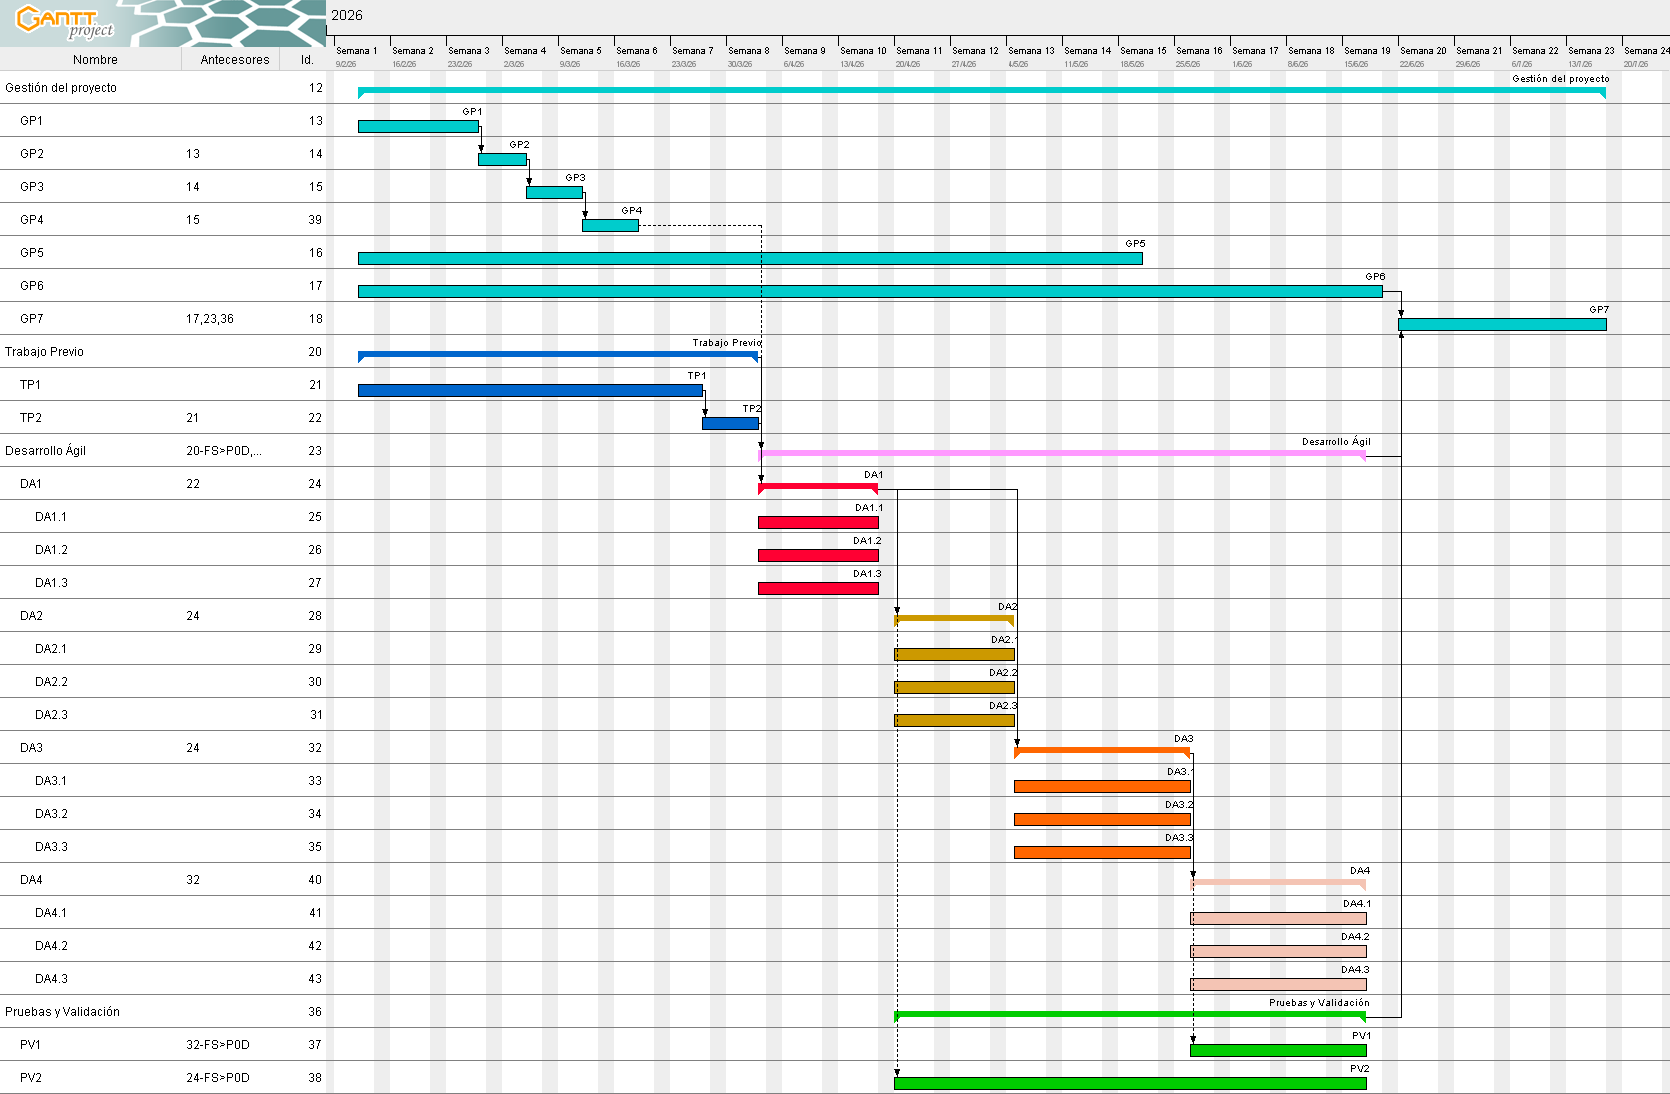
\includegraphics[width=1.5\textwidth]{imagenes/Gant_Lliurament2.png}
     \caption{Diagrama de Gantt, creado con el software \textit{GanttProject}. Generación propia}
     \label{fig:gantt}
    \end{figure}
\end{landscape}

\subsubsection{Revisión de la planificación inicial}
\label{sec:revision_planificacion}

La planificación establecida en el GEP estructuraba el desarrollo en cuatro sprints centrados en la construcción de agentes desde cero. El cambio de alcance producido al finalizar TP1 implicó una redistribución del contenido de los sprints, manteniendo el número de fases y el total de horas estimado (~540h) sin desviación significativa.

\begin{table}[H]
\centering
\begin{tabularx}{\textwidth}{>{\centering\arraybackslash}p{1cm} >{\raggedright\arraybackslash}X >{\raggedright\arraybackslash}X}
    \toprule
    \textbf{Sprint} & \textbf{Planificación GEP} & \textbf{Planificación final} \\
    \midrule
    \textbf{DA1} & Agentes Architect, Developer y Reviewer desde cero & Plugin colbPowers base: constitution.md, features.md, orquestador \\
    \textbf{DA2} & Métricas de evaluación integradas en el agente Reviewer & Subagentes especializados + scripts de radon como evaluación manual independiente \\
    \textbf{DA3} & AgentSkills e integración MCP & Ampliación de MCPs y refinamiento del flujo colbPowers --- sin cambio significativo \\
    \textbf{DA4} & Information Retrieval y MCPs avanzados & Módulo de toma de requerimientos (Azure Speech + LangChain/Tavily) y módulo de seguimiento del cliente \\
    \bottomrule
\end{tabularx}
\caption{Comparativa entre la planificación del GEP y la planificación final ejecutada. Elaboración propia.}
\label{tab:comparativa_planificacion}
\end{table}

La justificación de estos cambios es consistente con lo descrito en la sección \ref{sec:revision_alcance}: la adopción de \textit{superpowers} redujo el esfuerzo necesario en DA1 y DA2, liberando capacidad que se reinvirtió en DA4 para los módulos complementarios. Las horas totales por fase se mantienen dentro del margen estimado; en la tabla \ref{tab:resumen_tareas} se recogen las horas estimadas, y en el apartado de gestión económica (\ref{sec:revision_costes}) se cuantifica el impacto económico real.

\newpage

\subsection{Gestión de riesgos: Planes alternativos y obstáculos}
\label{sec:gestion_riesgos}
Durante la planificación y ejecución de este proyecto, se han identificado diversos obstáculos potenciales inherentes al desarrollo con IA. A continuación, se detallan estos riesgos junto con sus respectivos planes alternativos, tal y como dictan las buenas prácticas de gestión ágil de proyectos. En el apartado \ref{sec:imprevistos} se cuantifica el coste económico estimado de cada uno de estos imprevistos.

\subsubsection{Riesgo 1: Cambios repentinos en los requerimientos por parte de la empresa}
\label{sec:riesgo1}
\begin{itemize}
    \item \textbf{Probabilidad:} Baja / Media (40\%)
    \item \textbf{Tareas afectadas:} Principalmente las fases de Desarrollo Ágil (\textbf{DA1--DA4}), ya que un cambio de requerimientos puede invalidar trabajo ya implementado en cualquier \textit{Sprint}. También se ve afectada la tarea \textbf{GP5} (Reuniones de Seguimiento), que deberá absorber sesiones extraordinarias de re-planificación, y potencialmente \textbf{PV} si los cambios implican redefinir los criterios de validación.
    \item \textbf{Tareas alternativas (Plan B):} Re-evaluación del \textit{Sprint Backlog} actual, congelación del código afectado y re-planificación de los objetivos en una reunión extraordinaria para el siguiente \textit{Sprint}.
    \item \textbf{Afectación a la duración total:} Retraso estimado de 15 horas sobre la planificación original, absorbible en la fase de pruebas (PV).
    \item \textbf{Recursos adicionales necesarios:} Horas extra del autor y disponibilidad del Director del proyecto para una sesión de rediseño.
    \item \textbf{Resultado:} Este riesgo se materializó durante la fase TP1. El mecanismo de revisión de sprint absorbió el cambio de alcance de forma controlada, reorientando el Sprint Backlog sin comprometer la planificación global ni el presupuesto estimado.
\end{itemize}

\subsubsection{Riesgo 2: Bloqueo tecnológico (Vendor Lock-in) por cambio de precios o políticas en las APIs de los LLMs}
\label{sec:riesgo2}
\begin{itemize}
    \item \textbf{Probabilidad:} Baja / Media (30\%) \cite{opara_vendor_lockin_2016}
    \item \textbf{Tareas afectadas:} El impacto recae principalmente sobre \textbf{DA3} (Habilidades e Integración MCP), donde se construyen los módulos de conexión con las APIs, y sobre \textbf{DA4} (Recuperación de Información y Refinamiento), que depende de integraciones avanzadas con proveedores externos. En menor medida, también puede afectar a \textbf{DA1} si el agente base necesita ser reconectado a un proveedor distinto.
    \item \textbf{Tareas alternativas (Plan B):} Migración del motor cognitivo del sistema hacia modelos \textit{Open Source} (ej. LLaMA o Mistral) ejecutados en local o a través de proveedores alternativos, modificando el módulo de conexión (\textit{wrapper}).
    \item \textbf{Afectación a la duración total:} Aumento de 20 horas en la fase de Integración MCP (DA3).
    \item \textbf{Recursos adicionales necesarios:} Tiempo extra de desarrollo y posible necesidad de hardware local con mayor capacidad de procesamiento (GPU) temporal.
\end{itemize}

\subsubsection{Riesgo 3: Documentación interna insuficiente para la generación autónoma de código estructurado}
\label{sec:riesgo3}
\begin{itemize}
    \item \textbf{Probabilidad:} Media (50\%)
    \item \textbf{Tareas afectadas:} Afecta directamente a \textbf{DA1} (implementación del agente Developer, cuya capacidad de escritura se reduciría), \textbf{DA2} (las métricas de evaluación perderían parte de su utilidad si el agente no genera código autónomamente) y \textbf{PV2} (el bucle completo \textit{Human in the Loop} requeriría una mayor intervención manual del autor, alterando la naturaleza de la validación).
    \item \textbf{Tareas alternativas (Plan B):} Reducción del alcance del sistema (\textit{scope downgrade}). Se limitarán las capacidades de escritura del agente \textit{Developer}. El desarrollador humano (usuario) asumirá la implementación directa del código base, mientras que los agentes (\textit{Architect} y \textit{Reviewer}) se reorientarán exclusivamente a tareas de lectura: documentar, auditar la estructura y comprobar la calidad del código manual contra la especificación original.
    \item \textbf{Afectación a la duración total:} Impacto temporal neutro. Las horas ahorradas en el desarrollo de \textit{skills} complejas de escritura para los agentes se reinvertirán en la codificación manual por parte del autor durante el bucle de pruebas (PV).
    \item \textbf{Recursos adicionales necesarios:} Mayor carga de programación manual y esfuerzo cognitivo por parte del autor, al delegar menos carga de implementación en la inteligencia artificial.
\end{itemize}

\subsubsection{Riesgo 4: Limitaciones de control sobre el flujo de orquestación en el ecosistema IDE}
\label{sec:riesgo4}
\begin{itemize}
    \item \textbf{Probabilidad:} Media / Alta (65\%)
    \item \textbf{Tareas afectadas:} Afecta directamente a \textbf{DA1} (implementación del MVP sobre el entorno IDE) y a \textbf{DA3} (Habilidades e Integración MCP), donde se construyen los módulos de orquestación entre agentes. Si las restricciones del IDE resultan insalvables, estas tareas deberán ser rediseñadas.
    \item \textbf{Tareas alternativas (Plan B):} Rediseño de los \textit{prompts} de cada agente para que sean más breves, concisos y con un alcance muy acotado, reduciendo así la tendencia del modelo a desviarse del comportamiento esperado. En este escenario, la coordinación entre agentes recae explícitamente sobre el desarrollador humano, que actúa como orquestador manual del flujo. El inconveniente de esta solución es que exige que el usuario conozca con precisión el proceso de trabajo del sistema para dirigir correctamente a cada agente, lo que aumenta la curva de aprendizaje de la herramienta.
    \item \textbf{Afectación a la duración total:} Aumento estimado de 20 horas en \textbf{DA3} para rediseñar y ajustar los \textit{prompts} de los agentes afectados y documentar el flujo de coordinación manual para el usuario.
    \item \textbf{Recursos adicionales necesarios:} Tiempo de diseño de \textit{prompts} por parte del autor y elaboración de documentación del flujo de uso dirigida al desarrollador.
    \item \textbf{Resultado:} Este riesgo se manifestó parcialmente. Los mecanismos nativos de extensibilidad de ClaudeCode y OpenCode (MCP, hooks, skills) resultaron suficientes para implementar el flujo de trabajo requerido.
\end{itemize}

\subsubsection{Riesgo 5: Desbordamiento de la ventana de contexto en proyectos grandes}
\label{sec:riesgo5}
\begin{itemize}
    \item \textbf{Probabilidad:} Baja / Media (35\%)
    \item \textbf{Tareas afectadas:} Impacta principalmente en \textbf{DA4} (Recuperación de Información y Refinamiento), cuyo objetivo específico es abordar este problema mediante técnicas de \textit{Information Retrieval}. Si se manifiesta antes, también puede bloquear el avance de \textbf{DA1} y \textbf{DA3}, al impedir que los agentes mantengan suficiente contexto para operar correctamente.
    \item \textbf{Tareas alternativas (Plan B):} Aplicar dos estrategias complementarias de reducción de contexto. La primera consiste en implementar resúmenes automáticos o manuales de la conversación, descartando el historial detallado y reteniendo únicamente las decisiones clave ya tomadas. La segunda estrategia consiste en aislar al máximo el alcance de cada agente: en lugar de proporcionar contexto global del proyecto, cada agente opera exclusivamente sobre la \textit{feature} o módulo que tiene asignado, desconociendo intencionadamente el resto de la implementación. Esto mantiene la ventana de contexto acotada y manejable incluso en proyectos grandes.
    \item \textbf{Afectación a la duración total:} Impacto absorbible dentro de las 80 horas ya asignadas a \textbf{DA4}, aunque podría suponer un retraso de hasta 15 horas adicionales si la solución de aislamiento requiere rediseñar la estructura de memoria del sistema.
    \item \textbf{Recursos adicionales necesarios:} Ninguno adicional si se resuelve dentro de \textbf{DA4}; posibles horas extra del autor si la estrategia de aislamiento debe adelantarse a \textit{Sprints} anteriores.
\end{itemize}

\subsubsection{Riesgo 6: Exceso de fricción en el bucle de desarrollo por auditorías demasiado estrictas}
\label{sec:riesgo6}
\begin{itemize}
    \item \textbf{Probabilidad:} Baja (30\%)
    \item \textbf{Tareas afectadas:} Afecta a \textbf{DA3} (implementación del agente Reviewer y sus políticas de auditoría) y a \textbf{PV2} (pruebas del bucle completo \textit{Human in the Loop}), donde se evalúa empíricamente si el sistema resulta usable o frustrante para el desarrollador.
    \item \textbf{Tareas alternativas (Plan B):} Rediseño del agente \textit{Reviewer} para implementar niveles de severidad en las auditorías (errores críticos bloqueantes vs. advertencias no bloqueantes), permitiendo al usuario continuar el desarrollo ante desviaciones menores y reservando los bloqueos para incumplimientos graves de la especificación.
    \item \textbf{Afectación a la duración total:} Aumento de aproximadamente 10 horas en \textbf{DA3} para recalibrar y probar los umbrales de tolerancia del agente \textit{Reviewer}.
    \item \textbf{Recursos adicionales necesarios:} Sesiones de prueba adicionales con el autor actuando como usuario final para validar que el nuevo umbral resulta equilibrado.
\end{itemize}

\newpage

\subsection{Gestión económica}
\label{sec:gestion_economica}
En este apartado plantearemos los distintos costes que se prevé que aparecerán a lo largo del desarrollo del proyecto.

\subsubsection{Coste del personal}
\label{sec:coste_personal}
Aplicando el \textit{feedback} de la anterior entrega de GEP, vamos a dividir este apartado en distintos roles. Cada uno tendrá un coste por hora determinado, y visitando el diagrama de Gantt y las tablas con las horas asignadas a cada tarea y sus recursos personales adjuntados, calcularemos el total de cada uno de estos roles. Adicionalmente, se mostrarán tanto los salarios netos como los brutos - añadida la contribución de 30\verb|%| a la Seguridad Social (SS) -, y cuando se haga la suma total de los costes, se utilizará obviamente el salario bruto.

\begin{table}[H]
    \centering
    \begin{tabularx}{\textwidth}{X c c}
         \toprule
         \textbf{Rol} & \textbf{Salario Neto} & \textbf{Salario Bruto (+ SS)}\\
         \midrule
         \textbf{Jefe del Proyecto (Programador senior)} & 20,15€/h & 26,20€/h \\
         \textbf{Investigador y documentador} & 16,04€/h & 20,85€/h \\
         \textbf{Programador junior} & 11,48€/h & 14,92€/h \\
         \textbf{Testers} & 14,72€/h & 19,17€/h \\
         \bottomrule
    \end{tabularx}
    \caption{Costes de personal por hora según el rol asumido. Elaboración propia. Basada en información extraída de \cite{indeed_salarios}.}
    \label{tab:costes_personal}
\end{table}

\subsubsection{Coste por actividad}
\label{sec:coste_actividad}
Repasaremos las actividades presentadas en el entregable anterior, estudiaremos los recursos humanos invertidos en dicha actividad, y calcularemos el coste de cada una.
\paragraph{Gestión del proyecto}
\label{sec:coste_gp}
Esta se ha estimado que durará unas 167 horas en total. Dando por hecho que se desarrolla en un 25\verb|%| por el \textit{Jefe del Proyecto} y el restante 75\verb|%| por el \textit{Investigador/Documentador}, el coste humano de esta tarea es de: 
\begin{equation}
\centering
Coste GP = (0{.}25*26{.}2 \verb|€|/h + 0{.}75*20{.}85 \verb|€|/h)*167h = 3705{.}32\verb|€|
\end{equation}
\paragraph{Trabajo Previo}
\label{sec:coste_tp}
Esta actividad se estima que es de unas 50 horas. Requiere un estudio del estado del arte, y planificación del flujo del funcionamiento del proyecto. Las 30 horas de investigación del estudio del arte podrían estar desarolladas por el \textit{Investigador/Desarrollador}, mientras que la planificación del proyecto se llevaría a cabo por el \textit{Jefe del Proyecto}, por lo que 20 horas de su parte.
\begin{equation}
    Coste TP = 20h * 26{.}2\verb|€/h| + 30h * 20{.}85\verb|€|/h = 1149{.}5\verb|€|
\end{equation}
\paragraph{Desarrollo Ágil}
\label{sec:coste_da}
Como se hizo en la entrega anterior, el desarrollo ágil (DA) se dividirá en DA1, DA2, DA3 y DA4. Basándonos en la naturaleza de cada iteración, repartiremos la carga de trabajo entre los distintos roles definidos para estimar su coste:

\begin{itemize}
    \item \textbf{DA1 (Sprint 1 - MVP colbPowers):} Consta de 50 horas en total. Al tratarse de la configuración del plugin e implementación del agente orquestador base, asignaremos la totalidad de estas horas al \textit{Programador junior}.
    \begin{equation*}
        Coste DA1 = 50h * 14{.}92\verb|€|/h = 746\verb|€|
    \end{equation*}
    
    \item \textbf{DA2 (Sprint 2 - Subagentes y métricas):} Consta de 50 horas. Las 15 horas iniciales de investigación y configuración de radon serán llevadas a cabo por el \textit{Investigador y documentador}, mientras que las 35 horas restantes de implementación de subagentes y scripts recaerán sobre el \textit{Programador junior}.
    \begin{equation*}
        Coste DA2 = 15h * 20{.}85\verb|€|/h + 35h * 14{.}92\verb|€|/h = 836\verb|€|
    \end{equation*}
    
    \item \textbf{DA3 (Sprint 3 - Habilidades e Integración MCP):} De las 80 horas estimadas, 65 horas se dedicarán al desarrollo de \textit{Agent Skills} y protocolos MCP por parte del \textit{Programador junior}. Las 15 horas restantes, dedicadas al análisis de errores complejos y mejoras de estabilidad, requerirán la experiencia y supervisión del \textit{Jefe del Proyecto}.
    \begin{equation*}
        Coste DA3 = 65h * 14{.}92\verb|€|/h + 15h * 26{.}2\verb|€|/h = 1362{.}8\verb|€|
    \end{equation*}
    
    \item \textbf{DA4 (Sprint 4 - Módulos complementarios y refinamiento):} Cuenta con 80 horas totales. Asignaremos 20 horas al \textit{Investigador y documentador} para el diseño de los módulos de transcripción y seguimiento, y las 60 horas restantes al \textit{Programador junior} para la implementación de los módulos y el refinamiento final del sistema.
    \begin{equation*}
        Coste DA4 = 20h * 20{.}85\verb|€|/h + 60h * 14{.}92\verb|€|/h = 1312{.}2\verb|€|
    \end{equation*}
\end{itemize}

Sumando los costes de los cuatro \textit{Sprints}, obtenemos el coste total de los recursos humanos para la fase de Desarrollo Ágil:
\begin{equation}
    Coste DA = 746\verb|€| + 836\verb|€| + 1362{.}8\verb|€| + 1312{.}2\verb|€| = 4257\verb|€|
\end{equation}
\paragraph{Pruebas y Validación}
\label{sec:coste_pv}
Se estimó que en total esta tarea tomaría unas 60 horas a lo largo del proyecto. De estas 60 horas, todas ellas serian asignadas al Tester.

\begin{equation}
    Coste PV = 60h * 19{.}17\verb|€|/h = 1150{.}2\verb|€|
\end{equation}
\subsubsection{Costes genéricos}
\label{sec:costes_genericos}
En este apartado se referenciarán los costes que no se pueden asignar a una actividad específica, sino que están presentes a lo largo de todo el desarrollo. Estos incluyen los gastos de infraestructura, licencias de software y la amortización del equipo físico utilizado.

\paragraph{Costes estructurales}
\label{sec:costes_estructurales}
Los costes estructurales contemplan los gastos derivados del uso de un espacio de trabajo físico, así como los suministros básicos necesarios para llevar a cabo el desarrollo. Asumiendo que el proyecto tiene una duración estimada de 4,5 meses (desde mediados de febrero hasta principios de julio), se han estimado los siguientes gastos mensuales:

\begin{itemize}
    \item \textbf{Alquiler de la oficina:} Se asume el alquiler de un puesto en un espacio de \textit{coworking} o la parte proporcional de una oficina compartida, estimado en 150\verb|€|/mes. \cite{barcelona_coworking}
    \item \textbf{Electricidad:} Consumo derivado de los equipos informáticos, iluminación y climatización del espacio de trabajo, estimado en 50\verb|€|/mes. \cite{naturgy_precios}
    \item \textbf{Suministros adicionales:} Gastos de conectividad a Internet de alta velocidad y agua, calculados en 40\verb|€|/mes.
\end{itemize}

En total, el coste estructural mensual asciende a 240\verb|€|. Por lo tanto, el cálculo para los 4,5 meses de duración del proyecto es el siguiente:

\begin{equation}
    Coste Estructural = 4{.}5 \text{ meses} * 240\verb|€|/\text{mes} = 1080\verb|€|
\end{equation}

\paragraph{Costes de \textit{Software}}
\label{sec:costes_software}
El ecosistema tecnológico del proyecto se apoya en diversas herramientas. Afortunadamente, muchas de ellas cuentan con licencias gratuitas o versiones académicas sin coste (como Git, GitHub, VSCode, Odoo y Microsoft Teams). Sin embargo, el núcleo de este TFG requiere el uso de inteligencia artificial, lo que implica costes de suscripción y consumo de APIs (Claude Code, GitHub Copilot y servicios de Microsoft Azure / OpenAI).

Se ha estimado un presupuesto de consumo mensual para estas herramientas:
\begin{itemize}
    \item \textbf{GitHub Copilot:} 10\verb|€|/mes. \cite{github_pricing}
    \item \textbf{Claude:} 20\verb|€|/mes. \cite{claude_plans}
    \item \textbf{Consumo de APIs LLM (Azure/OpenAI/Anthropic):} 30\verb|€|/mes.
\end{itemize}
\begin{equation}
    Coste Software = (10\verb|€|/\text{mes}+ 20\verb|€|/\text{mes} + 30\verb|€|/\text{mes}) * 4{.}5 \text{ meses} = 270\verb|€|
\end{equation}

\paragraph{Costes de \textit{Hardware}}
\label{sec:costes_hardware}
Para calcular el coste del hardware, no se debe imputar el precio total de compra de los equipos, ya que estos no agotarán su vida útil exclusivamente con este proyecto. Se debe calcular su amortización. 

La fórmula de amortización se define dividiendo el precio del equipo entre sus horas de vida útil, y multiplicando el resultado por las horas dedicadas al TFG (estimadas en 540 horas en total). Se asume una vida útil de 4 años para los equipos informáticos (aproximadamente 220 días laborables al año, a 8 horas diarias = 7040 horas).

\begin{table}[H]
    \centering
    \begin{tabularx}{\textwidth}{X c c c}
         \toprule
         \textbf{Dispositivo} & \textbf{Precio Compra} & \textbf{Vida Útil (h)} & \textbf{Amortización (540h)} \\
         \midrule
         \textbf{Estación de trabajo (PC)} & 1500€ & 7040h & 115,06€ \\
         \textbf{Monitor externo} & 200€ & 7040h & 15,34€ \\
         \textbf{Periféricos (Teclado, ratón, audio)} & 100€ & 7040h & 7,67€ \\
         \midrule
         \textbf{Total} & \textbf{1800€} & --- & \textbf{138,07€} \\
         \bottomrule
    \end{tabularx}
    \caption{Cálculo de la amortización de los recursos de \textit{Hardware}. Elaboración propia.}
    \label{tab:amortizacion_hardware}
\end{table}

\begin{equation}
    Coste Hardware = 115{.}06\verb|€| + 15{.}34\verb|€| + 7{.}67\verb|€| = 138{.}07\verb|€|
\end{equation}

Sumando todos los componentes detallados en esta subsección, el total de costes genéricos asciende a:
\begin{equation}
    Total Genericos = 1080\verb|€| + 270\verb|€| + 138{.}07\verb|€| = 1488{.}07\verb|€|
\end{equation}

\subsubsection{Contingencias e imprevistos}
\label{sec:imprevistos}
En el desarrollo de cualquier proyecto de ingeniería informática, es fundamental disponer de un margen económico para hacer frente a posibles desviaciones temporales o problemas técnicos. Este margen se divide en dos partidas: las contingencias (para riesgos desconocidos) y los imprevistos (para riesgos ya identificados).

\paragraph{Contingencias}
\label{sec:contingencias}
La partida de contingencias actúa como un fondo de reserva general. Dado que el proyecto se basa en la integración de Inteligencia Artificial (LLMs) y herramientas en constante evolución, existe un grado de incertidumbre inherente. Aplicando las buenas prácticas de gestión de proyectos informáticos, se establece un margen de contingencia del 15\verb|%| sobre la suma total de los costes de personal y los costes genéricos estimados hasta el momento.
\begin{equation}
    Coste Contingencias = (Coste Personal + Coste Genericos) * 0{.}15
\end{equation}

\paragraph{Imprevistos}
\label{sec:imprevistos_sub}
Por otro lado, la partida de imprevistos cuantifica económicamente los riesgos específicos que ya fueron identificados y analizados en el Entregable 2. El coste que se añade al presupuesto se calcula multiplicando el coste del plan de acción alternativo (Plan B) por la probabilidad estimada de que el riesgo ocurra.

\begin{itemize} 
    \item \textbf{Riesgo 1: Cambios repentinos en los requerimientos.} La  probabilidad de ocurrencia se estimó como Baja/Media (40\verb|%|). El plan de mitigación contempla un retraso de 15 horas, implicando re-planificación y desarrollo. Asignaremos 5 horas al \textit{Jefe de Proyecto} (26,20\verb|€|/h) y 10 horas al \textit{Programador junior} (14,92\verb|€|/h).
    \begin{equation*}
        Coste R1 = ((5h * 26{.}20\verb|€|/h) + (10h * 14{.}92\verb|€|/h)) * 0{.}40 = 280{.}2\verb|€| * 0{.}40 = 112{.}08\verb|€|
    \end{equation*}
    \textbf{Impacto: Medio}

    \item \textbf{Riesgo 2: Bloqueo tecnológico (Vendor Lock-in) en APIs LLM.} La probabilidad es Baja/Media (30\verb|%|). El plan alternativo es la migración a modelos \textit{Open Source}, con un impacto de 20 horas de desarrollo (\textit{Programador junior}) y el alquiler puntual de hardware en la nube con GPU (estimado en 100\verb|€|).
    \begin{equation*}
        Coste R2 = ((20h * 14{.}92\verb|€|/h) + 100\verb|€|) * 0{.}30 = 398{.}4\verb|€| * 0{.}30 = 119{.}52\verb|€|
    \end{equation*}
    \textbf{Impacto: Medio}

    \item \textbf{Riesgo 3: Documentación interna insuficiente.} Probabilidad Media (50\verb|%|). El plan alternativo consiste en realizar un \textit{scope downgrade} (reducir capacidades de escritura de los agentes). Al tener un impacto temporal neutro (las horas no invertidas en IA se invierten en programación manual), no genera un coste económico extra en el presupuesto.
    \begin{equation*}
        Coste R3 = 0\verb|€| * 0{.}50 = 0\verb|€|
    \end{equation*}
    \textbf{Impacto: Bajo}

    \item \textbf{Riesgo 4: Limitaciones de control en el ecosistema IDE.} Probabilidad Media/Alta (65\verb|%|). El plan alternativo implica rediseñar los \textit{prompts} y documentar el flujo manual, con un impacto estimado de 20 horas en DA3: 10 horas de \textit{Programador junior} (14,92\verb|€|/h) y 10 horas de \textit{Investigador/Documentador} (20,85\verb|€|/h).
    \begin{equation*}
        Coste R4 = ((10h * 14{.}92\verb|€|/h) + (10h * 20{.}85\verb|€|/h)) * 0{.}65 = 357{.}7\verb|€| * 0{.}65 = 232{.}51\verb|€|
    \end{equation*}
    \textbf{Impacto: Medio}

    \item \textbf{Riesgo 5: Desbordamiento de la ventana de contexto.} Probabilidad Baja/Media (35\verb|%|). El plan alternativo puede requerir hasta 15 horas adicionales de \textit{Programador junior} (14,92\verb|€|/h) para rediseñar la estrategia de aislamiento de contexto.
    \begin{equation*}
        Coste R5 = (15h * 14{.}92\verb|€|/h) * 0{.}35 = 223{.}8\verb|€| * 0{.}35 = 78{.}33\verb|€|
    \end{equation*}
    \textbf{Impacto: Bajo}

    \item \textbf{Riesgo 6: Exceso de fricción en el bucle de desarrollo.} Probabilidad Baja (30\verb|%|). El plan alternativo requiere aproximadamente 10 horas adicionales de \textit{Programador junior} (14,92\verb|€|/h) en DA3 para recalibrar los umbrales del agente \textit{Reviewer}.
    \begin{equation*}
        Coste R6 = (10h * 14{.}92\verb|€|/h) * 0{.}30 = 149{.}2\verb|€| * 0{.}30 = 44{.}76\verb|€|
    \end{equation*}
    \textbf{Impacto: Bajo}
\end{itemize}

Sumando los valores obtenidos, calculamos el fondo total reservado para imprevistos:
\begin{equation}
    Total Imprevistos = 112{.}08\verb|€| + 119{.}52\verb|€| + 0\verb|€| + 232{.}51\verb|€| + 78{.}33\verb|€| + 44{.}76\verb|€| = 587{.}20\verb|€|
\end{equation}

\subsubsection{Coste total}
\label{sec:coste_total}
Una vez estimados todos los gastos asociados al desarrollo del proyecto, tanto directos (personal) como indirectos (genéricos), y habiendo reservado los fondos necesarios para contingencias e imprevistos, podemos definir el presupuesto final. 

A continuación, se presenta una tabla resumen con la consolidación de todas las partidas económicas calculadas previamente:

\begin{table}[H]
    \centering
    \begin{tabular}{l c}
         \toprule
         \textbf{Concepto} & \textbf{Coste Estimado} \\
         \midrule
         Coste de Personal (GP, TP, DA, PV) & 10.262,02€ \\
         Costes Genéricos (Estructurales, Software, Hardware) & 1.488,07€ \\
         \midrule
         \textbf{Subtotal (Base del proyecto)} & \textbf{11.750,09€} \\
         \midrule
         Contingencias (15\% sobre el Subtotal) & 1.762,52€ \\
         Imprevistos (Riesgos evaluados) & 587,20€ \\
         \midrule
         \textbf{PRESUPUESTO TOTAL} & \textbf{14.099,81€} \\
         \bottomrule
    \end{tabular}
    \caption{Presupuesto total estimado del proyecto. Elaboración propia.}
    \label{tab:coste_total}
\end{table}

\subsubsection{Revisión de los costes iniciales}
\label{sec:revision_costes}

El presupuesto comprometido en el GEP ascendía a \textbf{14.099,81€}. El cambio de alcance producido durante TP1 tuvo un impacto económico prácticamente neutro: las horas previstas para construir agentes desde cero se redistribuyeron entre la investigación del ecosistema de extensibilidad (TP1 ampliado) y la implementación de los módulos complementarios (DA4 reorientado), sin incrementar el total de horas estimado. La redistribución de horas entre fases no alteró los costes de personal porque los roles implicados en las tareas nuevas son los mismos que en las tareas sustituidas. Los costes genéricos tampoco variaron de forma significativa: las herramientas nuevas incorporadas (Azure Speech Service, Tavily) están cubiertas por las suscripciones existentes de Colb.AI o tienen un coste marginal absorbible dentro de la partida de APIs LLM ya presupuestada. El presupuesto final se mantiene en \textbf{14.099,81€}.

\subsubsection{Control de gestión}
\label{sec:control_gestion}
Para asegurar la viabilidad económica del Trabajo de Fin de Grado y evitar que el proyecto supere el presupuesto establecido, es estrictamente necesario aplicar un control de gestión continuo. Al utilizar una metodología ágil (SCRUM), este control se realizará al finalizar cada iteración o \textit{Sprint}, así como en las reuniones de seguimiento estipuladas.

El control se basará en comparar los valores estimados en este documento con los gastos y horas reales consumidas. Para cada indicador se define su fórmula de cálculo y los criterios de actuación concretos en función de la magnitud de la desviación detectada:

\begin{itemize}
    \item \textbf{Desviación de horas por tarea:} Mide si se ha invertido más o menos tiempo del planificado en una tarea concreta.
    \begin{equation}
        Desviaci\acute{o}n\ Horas = Horas\ Estimadas - Horas\ Reales
    \end{equation}
    \textbf{Criterio de actuación:}
    \begin{itemize}
        \item Desviación entre 0 y $-$10\%: dentro del margen tolerable. Se registra como nota en la revisión del \textit{Sprint} pero no requiere acción inmediata.
        \item Desviación entre $-$10\% y $-$20\%: se analiza la causa en la reunión de seguimiento con el director y se ajusta la estimación de las tareas pendientes del mismo bloque.
        \item Desviación superior al $-$20\%: se convoca una sesión extraordinaria de re-planificación, se re-prioriza el \textit{Sprint Backlog} y se eliminan o posponen las subtareas de menor valor del incremento actual.
    \end{itemize}

    \item \textbf{Desviación de coste de personal:} Calcula el impacto económico de la desviación de horas, multiplicándolo por el salario bruto del rol implicado.
    \begin{equation}
        Desviaci\acute{o}n\ Coste\ Personal = (Horas\ Estimadas - Horas\ Reales) * Coste\ Rol
    \end{equation}
    \textbf{Criterio de actuación:}
    \begin{itemize}
        \item Desviación acumulada inferior a $-$300\verb|€|: absorbible con el fondo de contingencias (15\%), sin acción adicional.
        \item Desviación acumulada entre $-$300\verb|€| y $-$800\verb|€|: se activa el fondo de contingencias y se restringe el alcance de las tareas de menor prioridad del bloque en curso.
        \item Desviación acumulada superior a $-$800\verb|€|: se aplica un \textit{scope downgrade} formal, eliminando funcionalidades secundarias para reconducir el presupuesto hacia los objetivos críticos del proyecto.
    \end{itemize}

    \item \textbf{Desviación de costes genéricos:} Controla si herramientas de software, hardware o infraestructura han sufrido variaciones de precio (por ejemplo, subida de tarifas en las APIs de los LLMs).
    \begin{equation}
        Desviaci\acute{o}n\ Gen\acute{e}ricos = Coste\ Gen\acute{e}rico\ Estimado - Coste\ Gen\acute{e}rico\ Real
    \end{equation}
    \textbf{Criterio de actuación:}
    \begin{itemize}
        \item Desviación puntual inferior a $-$30\verb|€|/mes: se registra y monitoriza. Si persiste más de dos meses consecutivos, se revisan alternativas.
        \item Desviación sostenida o superior a $-$30\verb|€|/mes: se evalúa la sustitución de la herramienta afectada por una alternativa gratuita u \textit{open source} equivalente (por ejemplo, migrar a un proveedor de LLM alternativo en caso de subida de tarifas de APIs).
    \end{itemize}

    \item \textbf{Consumo del fondo de imprevistos:} Evalúa cuánto remanente queda del fondo de emergencias calculado. Si el resultado es negativo, significa que se ha agotado el presupuesto de seguridad.
    \begin{equation}
        Estado\ Imprevistos = Total\ Imprevistos\ Estimado - Coste\ Imprevistos\ Consumido
    \end{equation}
    \textbf{Criterio de actuación:}
    \begin{itemize}
        \item Remanente superior al 50\% (más de 183\verb|€| disponibles): situación bajo control, sin cambios en el plan.
        \item Remanente entre el 0\% y el 50\%: se congela el uso del fondo para nuevos imprevistos menores y se activa el fondo de contingencias para cubrir desviaciones adicionales.
        \item Remanente negativo (fondo agotado): se aplica de inmediato un \textit{scope downgrade} de las funcionalidades con mayor riesgo económico y se notifica al director del proyecto para valorar conjuntamente medidas extraordinarias.
    \end{itemize}
\end{itemize}

\newpage

\subsection{Informe de sostenibilidad}
\label{sec:sostenibilidad}

\subsubsection{Autoevaluación de la competencia}
\label{sec:autoevaluacion}
Tras realizar la encuesta de autoevaluación, identifico un perfil técnico sólido pero con carencias formativas en la gestión de la sostenibilidad. Uno de mis puntos fuertes es el compromiso con la eficiencia técnica y el orden del código (\textit{Green Computing}), lo que garantiza soluciones robustas y mantenibles a largo plazo. No obstante, el cuestionario ha evidenciado que durante la carrera me han faltado asignaturas que profundicen en métricas de sostenibilidad medioambiental, económica y social.

Esta falta de base académica ha sido mi principal punto débil al afrontar la estimación de costes y riesgos de este proyecto. Sin embargo, mediante un proceso de aprendizaje autónomo durante la planificación, he comprendido la importancia crítica de estos conceptos para gestionar adecuadamente un proyecto de cierto calibre como puede ser un TFG. Esta reflexión me ha permitido adoptar una visión más empática de la ingeniería, utilizando la metodología SDD no solo para buscar la eficiencia, sino para prevenir el \textit{burnout} y fomentar la sostenibilidad social del equipo.

Concretamente, en el bloque de métricas de impacto ambiental y social, comprendo de forma intuitiva conceptos básicos como la huella ambiental o el ciclo de vida de un producto, pero los marcos de medición más formalizados y los indicadores cuantitativos de impacto social eran prácticamente desconocidos para mí. Esta brecha fue evidente al tener que razonar sobre el impacto social de una herramienta de IA como la que propone este TFG.

El bloque donde partía con menor preparación era el de gestión económica: conceptos como las amortizaciones, el control de desviaciones presupuestarias o la estructura detallada de un presupuesto los he aprendido prácticamente desde cero durante la elaboración del proyecto, lo que ha supuesto el reto más importante a nivel de sostenibilidad de todo el GEP. En contraste, en lo relativo a los principios éticos y deontológicos del impacto de la IA, ya contaba con una conciencia bastante desarrollada antes de comenzar, al tratarse de un tema que me preocupa activamente como futuro ingeniero.
\\

\textit{Nota: Los contenidos de la matriz de sostenibilidad (PPP, Vida Útil y Riesgos) para cada una de las tres dimensiones se desarrollan a continuación en un formato narrativo en lugar de tabular, para facilitar la exposición de los conceptos.}

\subsubsection{Dimensión económica}
\label{sec:dimension_economica}
\textbf{PPP:} El coste total del proyecto se estima en 14.099,81€. Tras reflexionar sobre este presupuesto, considero que es realista y competitivo para un desarrollo de 540 horas que integra tecnologías punteras de IA. La optimización del gasto se logra mediante el uso de herramientas de código abierto y un modelo de pago por uso para las APIs, centrando la inversión en el valor del esfuerzo humano y la investigación.

\textbf{Vida Útil:} Actualmente, la industria aborda el desarrollo asistido por IA de forma impulsiva (Code-Driven), lo que reduce costes iniciales pero dispara los de mantenimiento debido a la deuda técnica. Esta solución basada en SDD mejora económicamente este escenario al reducir dicha deuda desde la fase de planificación. Consideramos que la adopción del sistema desarrollado en este TFG puede llegar a decrementar las horas de mantenimiento y desarrollo a largo plazo, al garantizar que toda implementación esté respaldada por una especificación validada y coherente con la arquitectura del proyecto. Idealmente, el ahorro en tiempo de comprensión y corrección de errores debería amortizar la inversión inicial del proyecto.

\textbf{Riesgos:} El principal riesgo económico durante la vida útil del sistema es la escalada de precios de las APIs de los LLMs. Una subida significativa de tarifas por parte de los proveedores (Anthropic, OpenAI) podría encarecer el coste de mantenimiento mensual estimado, comprometiendo la viabilidad económica de la herramienta a largo plazo. La mitigación consiste en que el diseño del sistema sea compatible con distintes proveedores, permitiendo migrar a distintos proveedores o alternativas más económicas.

\textbf{Mantenimiento:} El coste operativo tras la entrega es mínimo, estimado en aproximadamente 120€/mes. Este importe cubre los costes de suscripciones a las APIs de IA (GitHub, Anthropic, ...) y unas 4 horas mensuales de soporte técnico de un \textit{programador junior} para actualizaciones menores y ajustes varios.
\begin{equation}
    CosteMantenimiento = 60\verb|€|/mes + 4h/mes * 14{.}92\verb|€|/h = 119{.}68\verb|€|/mes
\end{equation}

\subsubsection{Dimensión social}
\label{sec:dimension_social}
\textbf{PPP:} A nivel personal, este proyecto es un catalizador en mi formación. Me permite consolidar conocimientos técnicos en la orquestación de LLMs y, simultáneamente, adquirir habilidades críticas en gestión económica y metodologías ágiles (SCRUM), competencias que han demostrado ser tan vitales como la propia programación.

\textbf{Vida Útil:} Existe una necesidad real en el mercado debido al creciente estrés y frustración profesional que genera trabajar con bases de código incoherentes. La metodología SDD mejora la calidad de vida de los programadores al obligar a establecer especificaciones claras, reduciendo el caos y fomentando un entorno laboral más estructurado y colaborativo.

\textbf{Riesgos:} El principal riesgo social es la resistencia por parte de los desarrolladores a adoptar una metodología más estructurada como SDD, especialmente en equipos con poca cultura de documentación previa. Si la herramienta se percibe como una carga burocrática en lugar de un asistente, podría ser abandonada o eludida, anulando su impacto positivo. La mitigación pasa por un diseño centrado en la usabilidad, que guie al programador en su uso.

\subsubsection{Dimensión ambiental}
\label{sec:dimension_ambiental}
\textbf{PPP:} El impacto ambiental proviene del consumo eléctrico de los equipos durante las 540 horas de trabajo y el uso de servidores en la nube para las APIs. Para minimizar este impacto, se ha optado por reutilizar hardware personal y planificar un desarrollo local mediante WSL que limite las peticiones innecesarias a la red durante las fases iniciales de pruebas.

\textbf{Vida Útil:} La evaluación experimental confirma que colbPowers multiplica el consumo de tokens por un factor de entre 2{,}9× y 4{,}5× respecto a los asistentes sin flujo SDD, debido al overhead estructural del proceso (generación de especificaciones, delegación a subagentes y revisiones sistemáticas). El balance ambiental neto a largo plazo depende de si la mejora demostrada en la calidad del código se traduce en una reducción equivalente en sesiones de depuración, reescritura y mantenimiento futuro, compensando así el sobrecoste por sesión de desarrollo. Esta hipótesis es plausible pero no ha podido verificarse en el alcance de este trabajo.

\textbf{Riesgos:} El principal riesgo ambiental, confirmado empíricamente, es que el overhead de tokens del flujo SDD no quede compensado por la reducción en ciclos de corrección posteriores. En ese escenario, el sistema tendría un impacto ambiental neto superior al de los asistentes sin flujo estructurado. Para evaluar este riesgo con rigor sería necesario un estudio longitudinal que mida el número total de sesiones de desarrollo hasta la entrega del producto, incluyendo las de mantenimiento.

\subsection{Leyes y regulaciones}
\label{sec:leyes_y_regulaciones}

\begin{description}
    \item \textbf{Reglamento europeo de inteligencia artificial (EU AI Act):} El sistema no pertenece a ninguna de las categorías de alto riesgo definidas en el Anexo~III del Reglamento~(UE)~2024/1689~\cite{euaiact2024}: no toma decisiones autónomas con impacto significativo sobre personas físicas, y el diseño Human-in-the-Loop garantiza supervisión humana en todas las acciones con consecuencias reales.

    \item \textbf{Propiedad intelectual del código generado: } La titularidad del software generado con asistencia de IA  depende del grado de intervención humana en el proceso creativo. Un uso puramente autónomo de la IA —sin especificación previa ni revisión humana— no genera derechos de autor reconocibles. Sin embargo, cuando  la IA actúa como herramienta asistida con intervención humana documentada, los derechos corresponden al autor humano, siempre que esa intervención quede acreditada. \cite{medinatamayo2025}

    El flujo Spec-Driven Development implementado en este proyecto sitúa explícitamente la generación de código en la categoría de IA asistida: el desarrollador define la especificación, valida el plan de implementación antes de que comience la escritura de código, y revisa el resultado entregado por el subagente. Toda esta intervención queda registrada en el repositorio git del proyecto, proporcionando la documentación requerida para acreditar la autoría humana. Por otro lado, colbPowers es una obra derivada de \textit{superpowers}, distribuido bajo licencia MIT, con contribuciones originales documentadas en el repositorio git del proyecto que constituyen la aportación diferencial del TFG.

    \item \textbf{Licencias de terceros y Convenio de Cooperación Educativa: } Todas las herramientas de terceros utilizadas en el proyecto —OpenCode, code-review-graph, LangChain— disponen de licencias open source que permiten el uso comercial. Las APIs de Anthropic, Azure y Google Gemini no utilizan los datos de entrada para entrenar modelos bajo sus planes de pago. Por otro lado, Copilot sí que entrena con los datos adquiridos durante las interacciones con sus modelos -Des de el 24 de abril de 2026- de forma predeterminada, pero es una opción que se puede desactivar facilmente \cite{rodriguez2026copilot}. El TFG se desarrolla en el marco de un Convenio de Cooperación Educativa entre la UPC y Colb.AI, que regula la propiedad intelectual del trabajo y la confidencialidad de la información de la empresa. Los proyectos reales utilizados en la validación experimental están sujetos a NDA; en la memoria únicamente se reportan métricas técnicas que no exponen información confidencial del cliente.
\end{description}

\newpage

\section{Módulos de Transcripción y Documentación}
\label{sec:modulos_transcripcion}

\subsection{Toma de Requerimientos}
\label{sec:toma_requerimientos_cap}
La toma de requerimientos es la primera fase del ciclo de vida de un proyecto de software. En este contexto, el objetivo es transformar las necesidades expresadas por el cliente en conversaciones informales en documentos de especificación técnica utilizables por el equipo de desarrollo. El proceso se articula en dos módulos independientes y secuenciales: en primer lugar, el módulo de transcripción convierte las reuniones en texto estructurado; a continuación, el módulo de procesamiento analiza ese texto y genera el plan de implementación. Cada módulo dispone de dos implementaciones complementarias, con el propósito de no depender de un único proveedor.

\subsubsection{Módulo de transcripción}
\label{sec:modulo_transcripcion}
Para que el módulo de procesamiento pueda operar, es necesario disponer previamente de una transcripción de la reunión con el cliente. Dependiendo del tipo de reunión, la forma de obtenerla difiere.

\paragraph{Reuniones telemáticas}
\label{sec:reuniones_telematicas}
Las principales plataformas de videoconferencia (Microsoft Teams, Google Meet, Zoom, entre otras) ofrecen transcripción automática integrada. Dado que cada participante habla desde su propio dispositivo y micrófono, la atribución de fragmentos de texto a cada hablante (diarización) es gestionada de forma nativa por la plataforma, sin necesidad de ningún procesamiento adicional. Para las reuniones telemáticas, se utiliza directamente la transcripción exportada por la plataforma correspondiente como entrada al módulo de procesamiento.

\paragraph{Reuniones presenciales}
\label{sec:reuniones_presenciales}
En el caso de las reuniones presenciales, no existe ninguna plataforma que genere una transcripción de forma automática. Para cubrir este caso, se graba el audio de la reunión y se procesa a posteriori mediante Azure Speech Service, el servicio de transcripción de audio proporcionado por el proveedor de servicios cloud de la empresa.

La característica técnica diferencial en este contexto es la diarización (\textit{speaker diarization}): el servicio no transcribe el audio como un bloque de texto continuo, sino que identifica a cada participante de forma independiente y etiqueta cada fragmento de texto con el hablante que lo pronunció. Esta atribución es especialmente relevante para la toma de requerimientos, ya que permite al módulo de procesamiento distinguir qué peticiones o restricciones provienen del cliente y cuáles son aclaraciones o comentarios del equipo técnico, mejorando la calidad del plan de implementación resultante.

\paragraph{Preprocesamiento del audio.}
Antes de enviar el audio al servicio de transcripción, se aplica un paso de compresión cuyo objetivo es doble: reducir el tamaño del fichero para minimizar costes de almacenamiento y transferencia, y garantizar que el proceso sea determinista. La función \texttt{downsample\_audio\_deterministic} utiliza \texttt{ffmpeg} para convertir el audio original a formato MP3 mono a 8\,kHz, eliminando metadatos y aplicando flags de codificación bit-exacta (\texttt{-bitexact}, \texttt{-map\_metadata -1}, \texttt{-id3v2\_version 0}). Gracias a estas garantías, el mismo archivo de entrada siempre produce exactamente los mismos bytes de salida y, por tanto, el mismo hash SHA-256. Este hash actúa como identificador único del contenido del audio a lo largo de todo el sistema.

\paragraph{Gestión idempotente mediante máquina de estados.}
El componente \texttt{SpeechToText} implementa un mecanismo idempotente apoyado en Azure Blob Storage. Al recibir un fichero de audio, se calcula su hash determinista y se consulta el fichero \texttt{state.txt} asociado en el contenedor de almacenamiento. El ciclo de vida de una transcripción sigue la siguiente secuencia de estados:

\begin{enumerate}
    \item \textbf{\texttt{just\_created}}: el audio aún no ha sido procesado. Se sube el fichero comprimido al blob, se genera una URL de acceso temporal con firma de acceso compartido (SAS), y se lanza el trabajo de transcripción por lotes.
    \item \textbf{\texttt{transcribing}}: la transcripción está en curso. Si se recibe una nueva solicitud para el mismo hash, el sistema devuelve inmediatamente un mensaje informativo sin lanzar un trabajo duplicado.
    \item \textbf{\texttt{transcribed}}: la transcripción ha concluido con éxito. El texto resultante se almacena en el blob y se devuelve una URL SAS de acceso al fichero.
\end{enumerate}

Este diseño garantiza que procesar dos veces el mismo audio no genere costes adicionales ni resultados duplicados.

\paragraph{Transcripción por lotes (\textit{Batch API}).}
La transcripción se realiza a través de la API REST de Azure Speech Service en su versión 3.2, concretamente el endpoint de \textit{batch transcription}. El componente \texttt{BatchTranscriptor} realiza tres pasos:

\begin{enumerate}
    \item \textbf{Envío del trabajo}: se realiza una petición \texttt{POST} al endpoint de transcripciones con la URL SAS del audio comprimido. La configuración incluye el idioma (español por defecto), el modo de puntuación automática y, cuando la diarización está habilitada, los parámetros \texttt{diarizationEnabled: true} junto con el rango esperado de hablantes (mínimo 2, máximo 5).
    \item \textbf{Sondeo del estado}: se consulta periódicamente el estado del trabajo (cada 5 segundos) hasta que la API reporta \texttt{Succeeded} o \texttt{Failed}.
    \item \textbf{Descarga y formateo del resultado}: una vez completado el trabajo, se descarga el fichero de resultados y se procesan las frases reconocidas (\texttt{recognizedPhrases}). Cuando la diarización está activa, cada frase se ordena cronológicamente según su \textit{offset} en formato ISO 8601 y se formatea como \texttt{[Speaker N]: texto}, produciendo una transcripción estructurada por hablante. Si la diarización no está disponible, se recurre al campo \texttt{combinedRecognizedPhrases} como fallback.
\end{enumerate}

\begin{figure}[H]
    \centering
    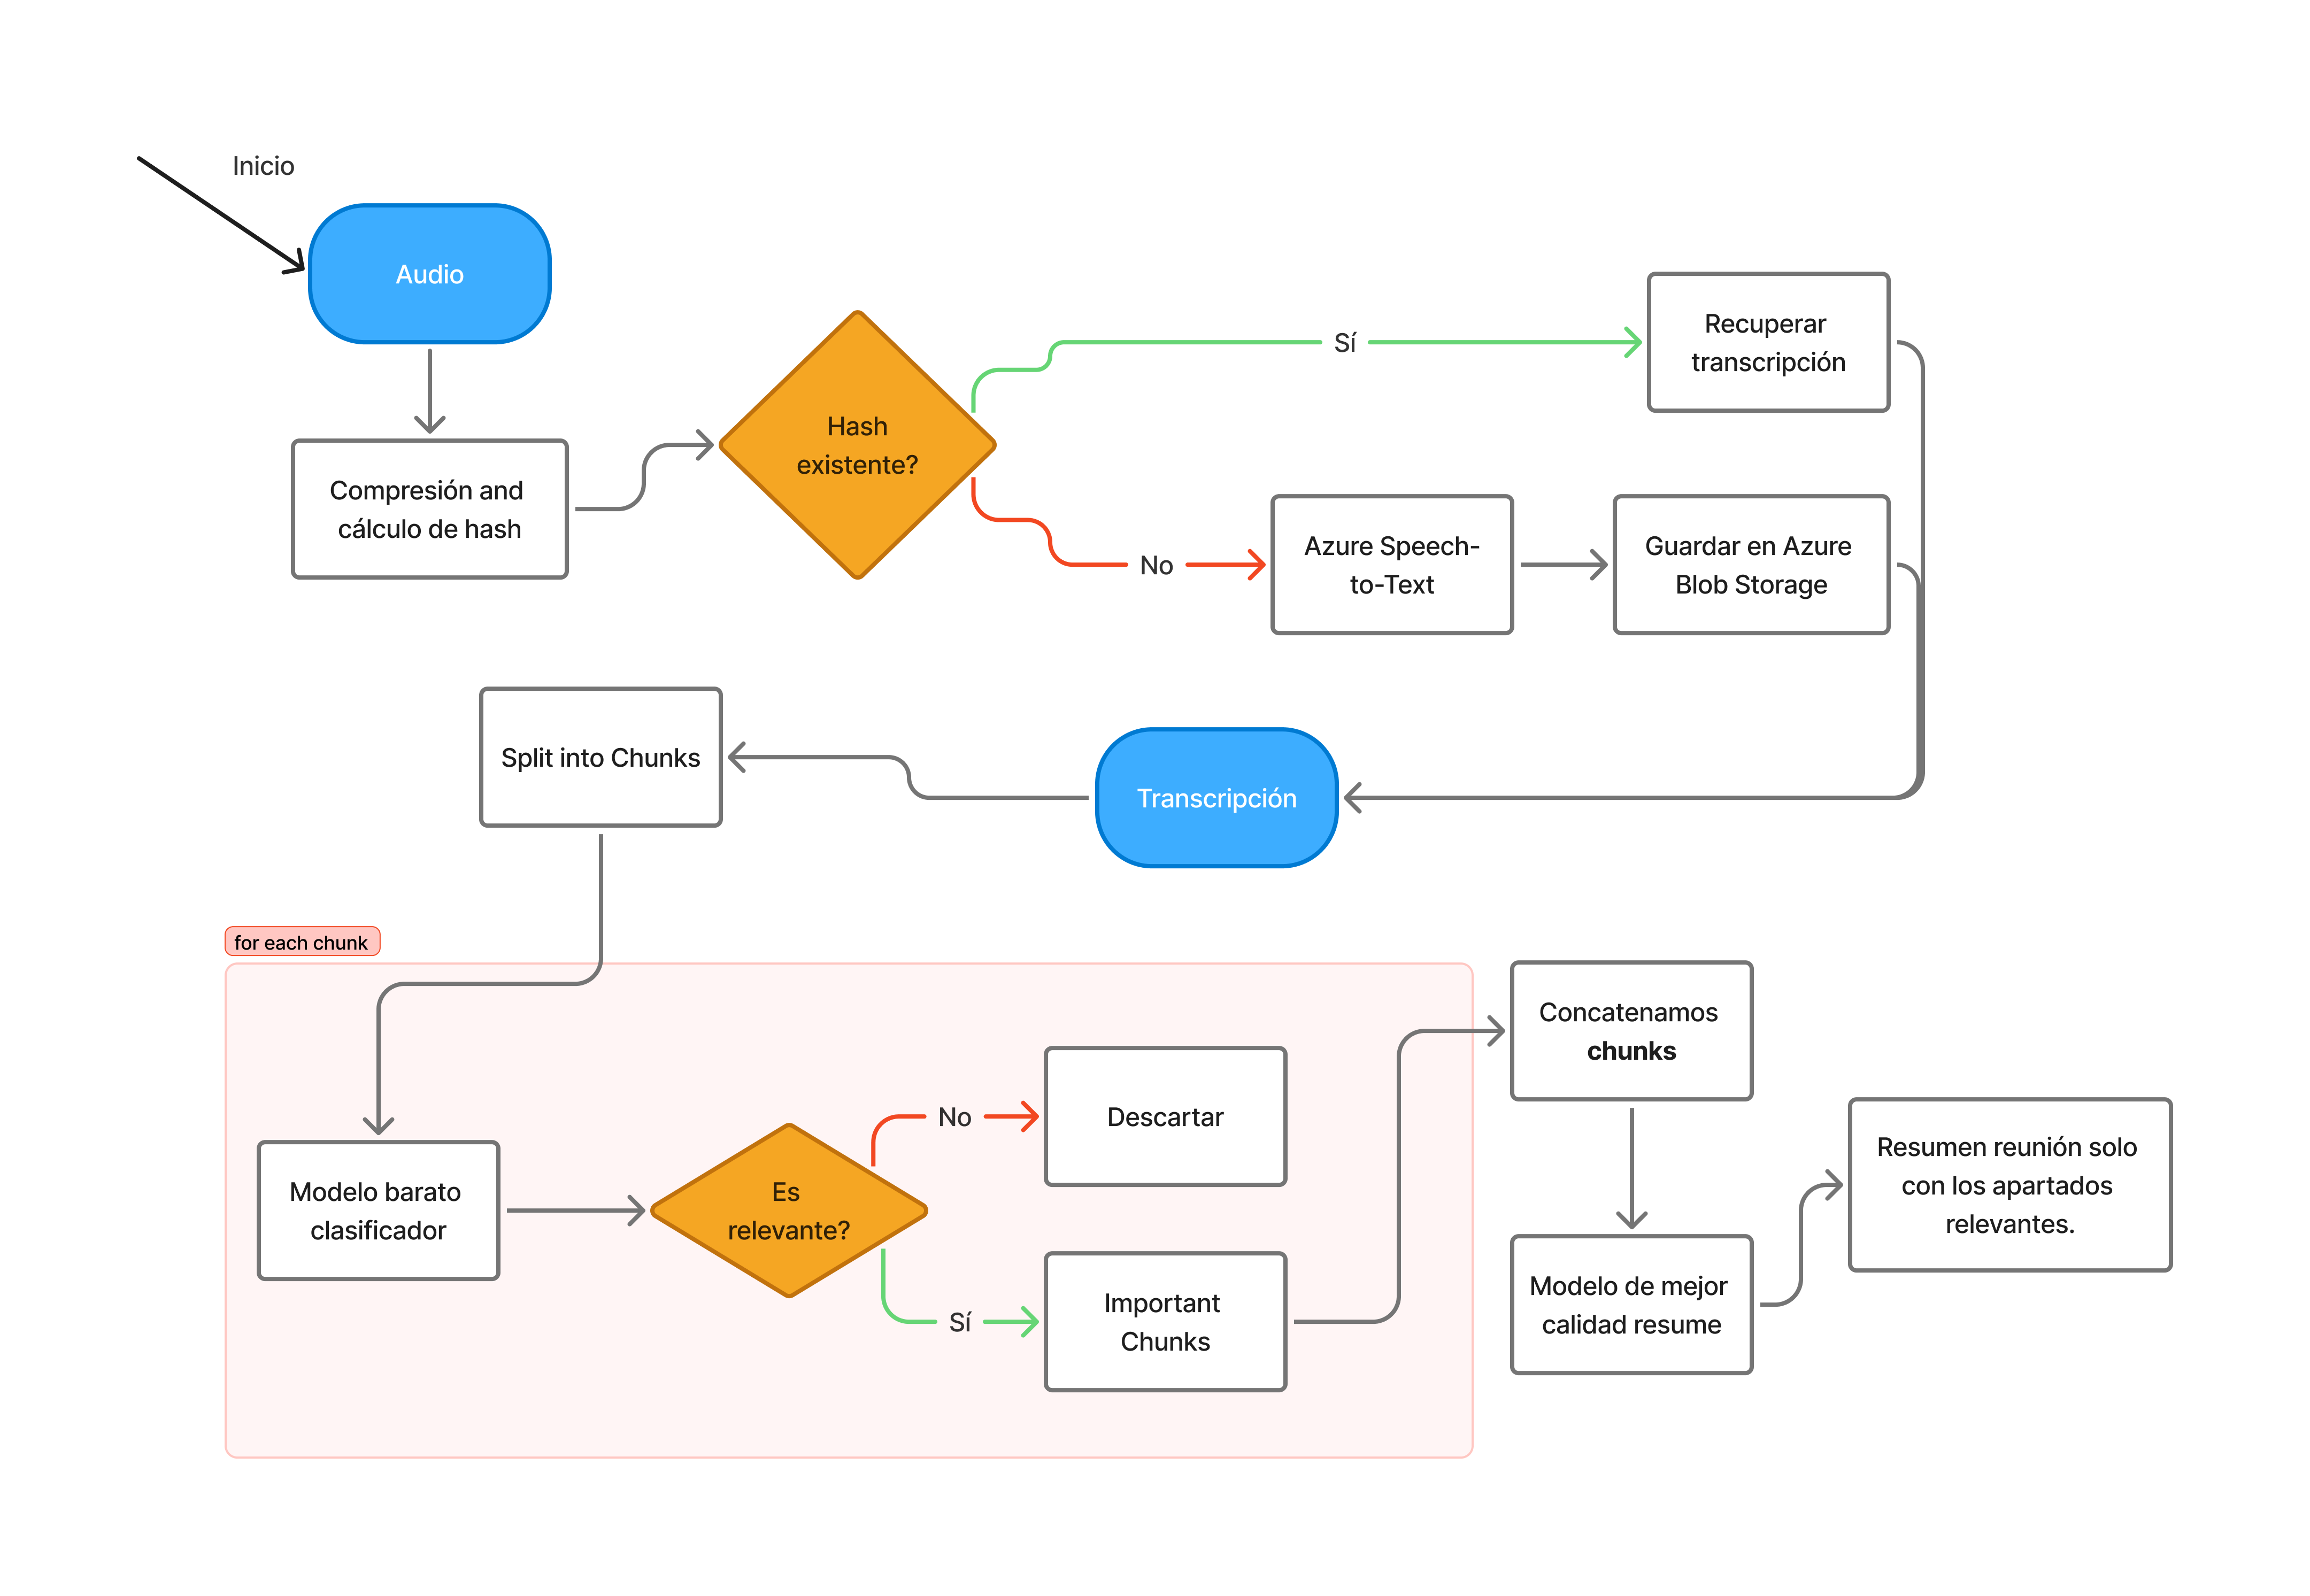
\includegraphics[width=1\textwidth]{imagenes/Transcription System.png}
    \caption{Diagrama de flujo de el proceso de transcripción. Generación propia.}
    \label{fig:skill_definition}
\end{figure}

\subsubsection{Módulo de procesamiento de requerimientos}
\label{sec:modulo_procesamiento}
Una vez disponible la transcripción (producida por cualquiera de las vías descritas en la sección anterior), el módulo de procesamiento la analiza y genera un plan de implementación estructurado. Este módulo también dispone de dos implementaciones: un enfoque basado en la plataforma Claude Cowork y una implementación propia en Python.

\paragraph{Enfoque mediante Claude Cowork}
  \label{sec:enfoque_claude_cowork}
  Claude Cowork es una herramienta de Anthropic orientada a la automatización de tareas en entorno de escritorio. 
  
  El modelo de uso se basa en el concepto de Skill: un workflow de automatización configurable que combina un prompt especializado con conexiones a herramientas, servicios externos y scripts personalizados.
  
  La skill recibe una entrada (por ejemplo, una transcripción de texto), las herramientas que puede invocar durante su ejecución (búsqueda en internet, lectura y escritura de archivos, llamadas a APIs externas, ejecución de scripts) y el formato de la salida que produce. A diferencia de un prompt ordinario enviado en una conversación, una skill encapsula el flujo de trabajo completo, con scripts y ejecutables incluidos dentro de la propia skill, y puede reutilizarse de forma consistente en cualquier proyecto sin necesidad de redefinirlo.
  
  \begin{figure}[H]
      \centering
      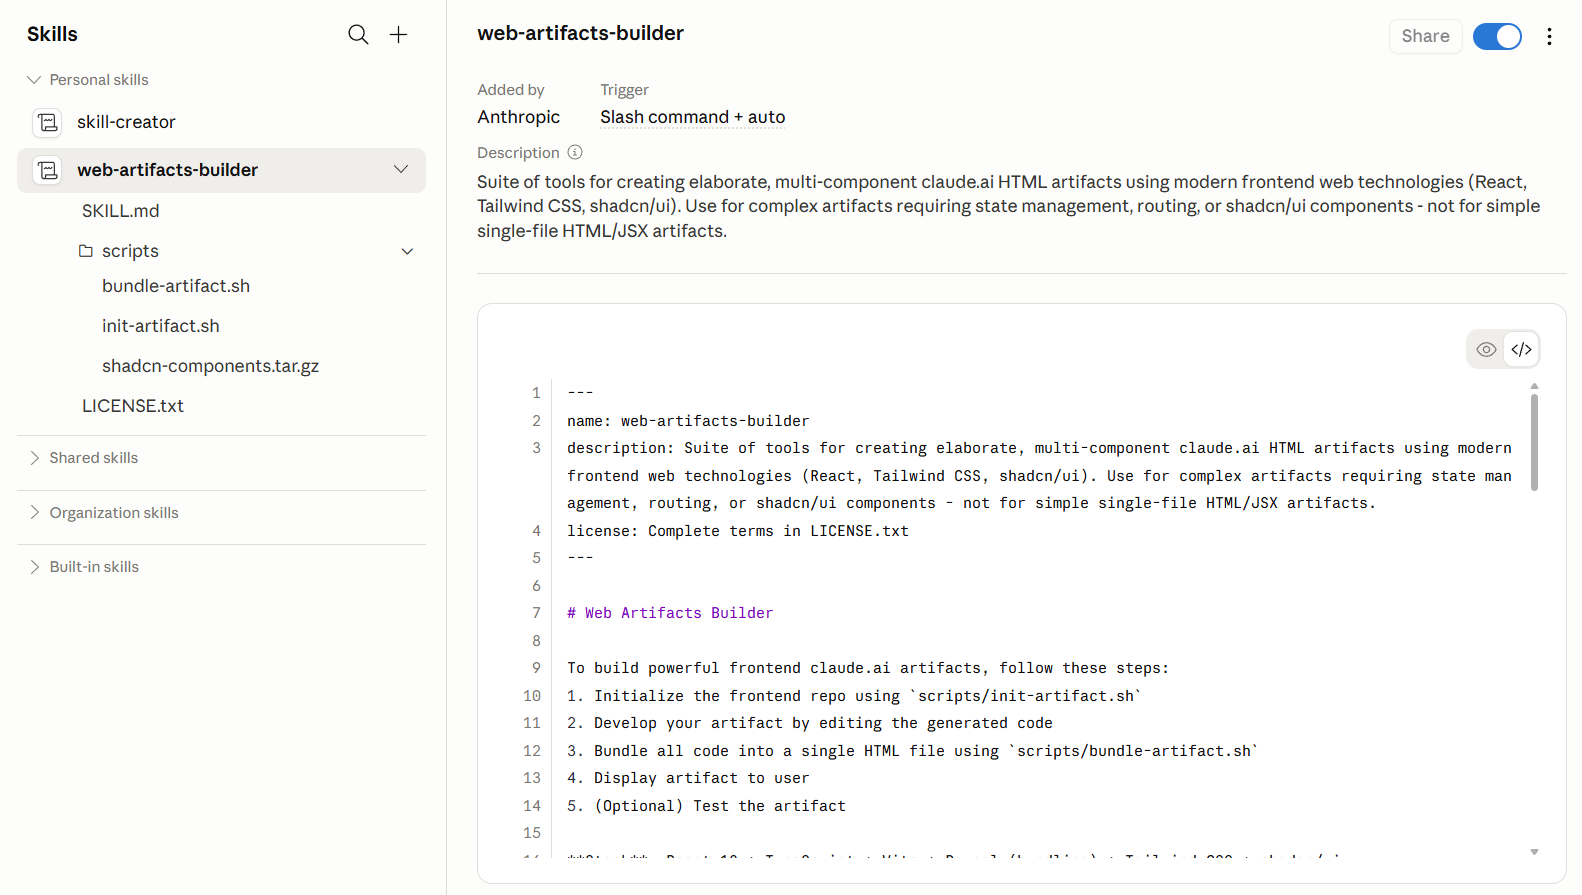
\includegraphics[width=1\textwidth]{imagenes/coworkSkills/skill_components_and_definition.png}
      \caption{Estructura de una skill en Claude Cowork.}
      \label{fig:skill_definition}
  \end{figure}

Se ha configurado una skill específica para la toma de requerimientos que implementa el siguiente flujo:

\begin{enumerate}
    \item El usuario proporciona a la skill la transcripción de la reunión con el cliente, notas informales o un resumen de las necesidades expresadas.
    \item La skill procesa el contexto y genera una visión global del proyecto (\textit{big picture}), identificando los componentes principales del sistema, las posibles tecnologías a emplear y las áreas de incertidumbre que requieren aclaración.
    \item Mediante las herramientas de búsqueda en internet integradas en Claude Cowork, el agente investiga las tecnologías propuestas y contrasta alternativas.
    \item El agente presenta al usuario las opciones tecnológicas encontradas para que seleccione las preferidas. El resultado es un documento de especificación inicial estructurado, listo para incorporarse al repositorio como punto de partida del desarrollo.
\end{enumerate}

Este enfoque es el preferido cuando se dispone de acceso a la plataforma Claude Cowork, dado que la integración con las herramientas de búsqueda y la calidad del razonamiento son superiores a los de la implementación propia.

\newpage

\paragraph{Implementación propia}
\label{sec:implementacion_propia_tr}
Con el objetivo de disponer de una alternativa de coste reducido e independiente de suscripciones comerciales, se ha desarrollado una aplicación Python que replica el proceso anterior. La aplicación está estructurada en módulos desacoplados y orquestada mediante LangChain.

\paragraph{Arquitectura.}
El núcleo de la aplicación es el módulo \texttt{transcription\_preprocessing}, que implementa la clase \texttt{TranscriptionProcessor} y coordina toda la lógica de negocio. El módulo recibe como entrada el texto de la transcripción y produce como salida un plan de implementación arquitectónico en formato Markdown.

El diseño emplea dos modelos de lenguaje con roles diferenciados: un modelo económico (Azure OpenAI) para las operaciones de alta frecuencia que no requieren razonamiento profundo, y un modelo de mayor capacidad (Google Gemini) para las tareas de síntesis y razonamiento arquitectónico. Esta estrategia de dos niveles optimiza el coste sin sacrificar la calidad del resultado final.

\paragraph{Pipeline de procesamiento.}
El flujo de procesamiento sigue cuatro fases secuenciales:

\paragraph{Fase 1: Chunking y filtrado:} la transcripción se divide en fragmentos de hasta 25.000 caracteres con un solapamiento de 1.200 caracteres y separadores jerárquicos (párrafos, líneas, frases), lo que permite procesar reuniones de larga duración sin superar los límites de contexto de los modelos. El modelo económico procesa cada fragmento de forma independiente y extrae únicamente el contenido relevante según un criterio configurable (por defecto, «requerimientos funcionales y reglas de negocio»), descartando saludos, divagaciones y contenido irrelevante. Los fragmentos sin contenido útil se descartan con la marca \texttt{SIN\_CONTENIDO\_RELEVANTE}.
    
\paragraph{Fase 2: Generación del plan de investigación:} el modelo de mayor capacidad analiza el texto filtrado e identifica las decisiones técnicas pendientes (elección de base de datos, framework, infraestructura). A partir de este análisis genera un plan de búsquedas estructurado con un máximo de tres \textit{queries}, para no saturar el límite de créditos del servicio de búsqueda.
    
\paragraph{Fase 3: Investigación web mediante Tavily:} Tavily opera como un motor de búsqueda semántica diseñado para agentes de IA, utilizando un \textit{pipeline} de filtrado híbrido. Primero, realiza una recuperación léxica para identificar URLs candidatas; posteriormente, mediante un motor de \textit{scraping} dinámico capaz de renderizar JavaScript, extrae el contenido relevante eliminando el ruido del HTML (anuncios, menús) y transformándolo en Markdown. El sistema procesa el texto mediante \textit{embeddings} vectoriales, calculando la similitud de coseno entre la consulta y los fragmentos extraídos para realizar un \textit{re-ranking} semántico en tiempo real. Finalmente, selecciona los segmentos con mayor densidad de información factual. Las \textit{queries} se ejecutan con búsqueda profunda (\texttt{search\_depth=advanced}), limitando los resultados a fuentes del último año y formateándolos como contexto estructurado.
    
\paragraph{Fase 4: Generación del plan arquitectónico:} el modelo de mayor capacidad combina la transcripción original con los resultados de la investigación y produce un documento de arquitectura en formato Markdown. El documento incluye el resumen de objetivos, la propuesta de stack tecnológico justificada con la investigación, los componentes clave del sistema y la hoja de ruta de implementación.


\paragraph{Bucle de refinamiento con \textit{Human in the Loop}.}
Una característica diferencial de la aplicación es la capacidad de refinamiento iterativo en cada fase. El usuario puede modificar el plan de investigación o el plan arquitectónico mediante instrucciones en lenguaje natural. El sistema mantiene un historial de conversación mediante la abstracción \texttt{MessagesPlaceholder} de LangChain, lo que permite que el modelo tome en cuenta el contexto de intercambios anteriores al procesar cada solicitud de refinamiento. Este mecanismo implementa el principio \textit{Human in the Loop} definido en los objetivos del proyecto.

\begin{figure}[H]
    \centering
    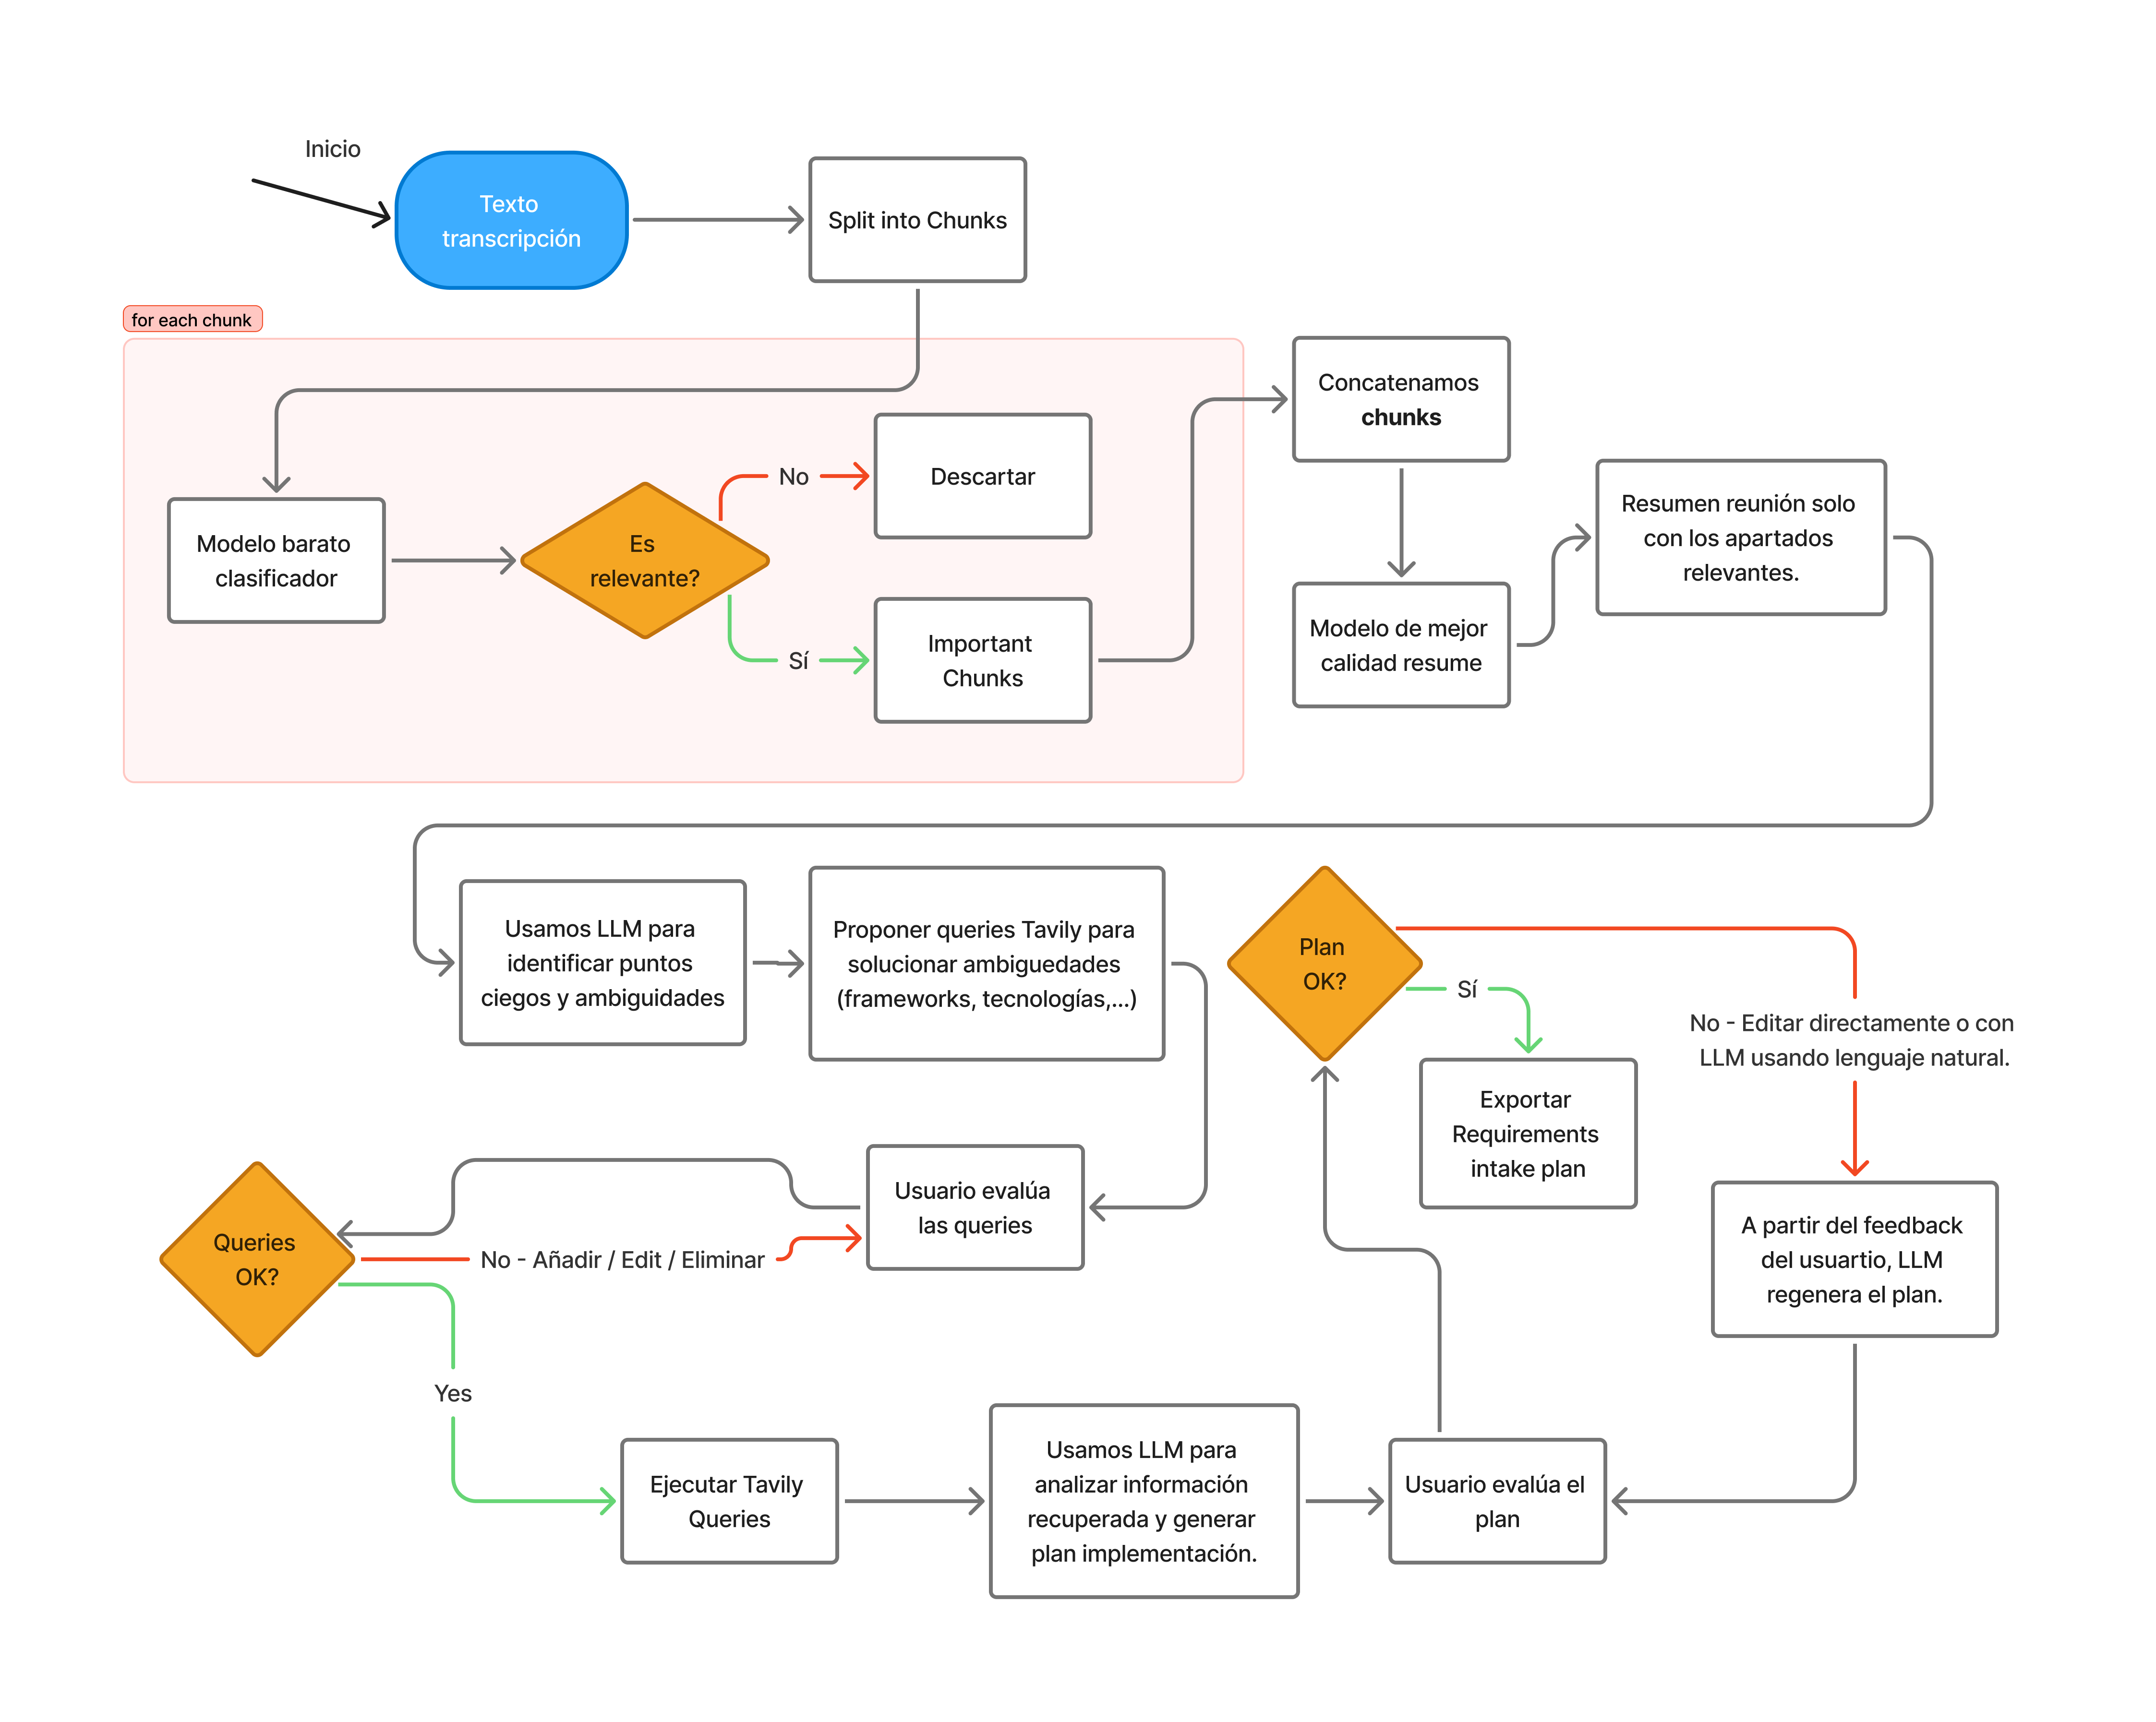
\includegraphics[width=1\textwidth]{imagenes/Requirements Intake System.png}
    \caption{Diagrama de flujo de el proceso generación de plan en la toma de requerimientos. Generación propia.}
    \label{fig:skill_definition}
\end{figure}

\newpage

\subsection{Seguimiento del Cliente}
\label{sec:seguimiento_cliente}
La tercera dimensión del proyecto aborda la automatización del seguimiento posterior a las reuniones periódicas con el cliente. El objetivo es minimizar el tiempo dedicado a la redacción de documentación de seguimiento y garantizar que los acuerdos alcanzados en cada reunión queden recogidos de forma estructurada y accesible para ambas partes.

\subsubsection{Generación de documentación con Claude Cowork}
\label{sec:generacion_doc_claude_cowork}
El flujo implementado mediante Claude Cowork se integra directamente con el proceso de reunión. Al finalizar cada reunión de seguimiento con el cliente, la transcripción o el resumen de lo acordado se proporciona como entrada a una skill de Claude Cowork desarrollada específicamente para este propósito. La skill procesa la información y genera de forma automática un documento Word estructurado que incluye los siguientes apartados:
\begin{itemize}
    \item Resumen de los temas tratados en la reunión.
    \item Decisiones tomadas y acuerdos alcanzados.
    \item Tareas asignadas al equipo de Colb.Ai con sus plazos correspondientes.
    \item Tareas o acciones que corresponden al cliente.
\end{itemize}
Este documento se genera y está disponible para ser enviado al cliente en el mismo momento en que finaliza la reunión, eliminando la latencia habitual en la producción de este tipo de documentación.

La skill aprovecha las capacidades nativas de Claude Cowork para acceder a herramientas de gestión de archivos en el entorno de escritorio, lo que le permite escribir directamente el documento en el directorio de trabajo del proyecto, integrándose de forma transparente en el flujo de gestión documental de la empresa.
\newpage
\subsubsection{Alternativa de código abierto}
\label{sec:alternativa_codigo_abierto}
De forma análoga al enfoque adoptado en la toma de requerimientos, se dispone de una alternativa de código abierto e independiente para los casos en que no se desee depender de la plataforma Claude Cowork. Esta alternativa se basa en una aplicación que combina un modelo de lenguaje de gran tamaño, accedido mediante API, con la biblioteca python-docx para la generación de documentos Word con formato estructurado. El flujo de la aplicación es equivalente al de la skill: a partir de la transcripción de la reunión, el modelo genera los distintos apartados del documento de seguimiento con un formato definido, que son entonces volcados al documento Word mediante la biblioteca de generación. Aunque la integración es menos fluida que la ofrecida por Claude Cowork, esta alternativa es igualmente válida para los casos de uso habituales y no incurre en costes de suscripción adicionales más allá del consumo de la API del modelo.

\begin{figure}[H]
    \centering
    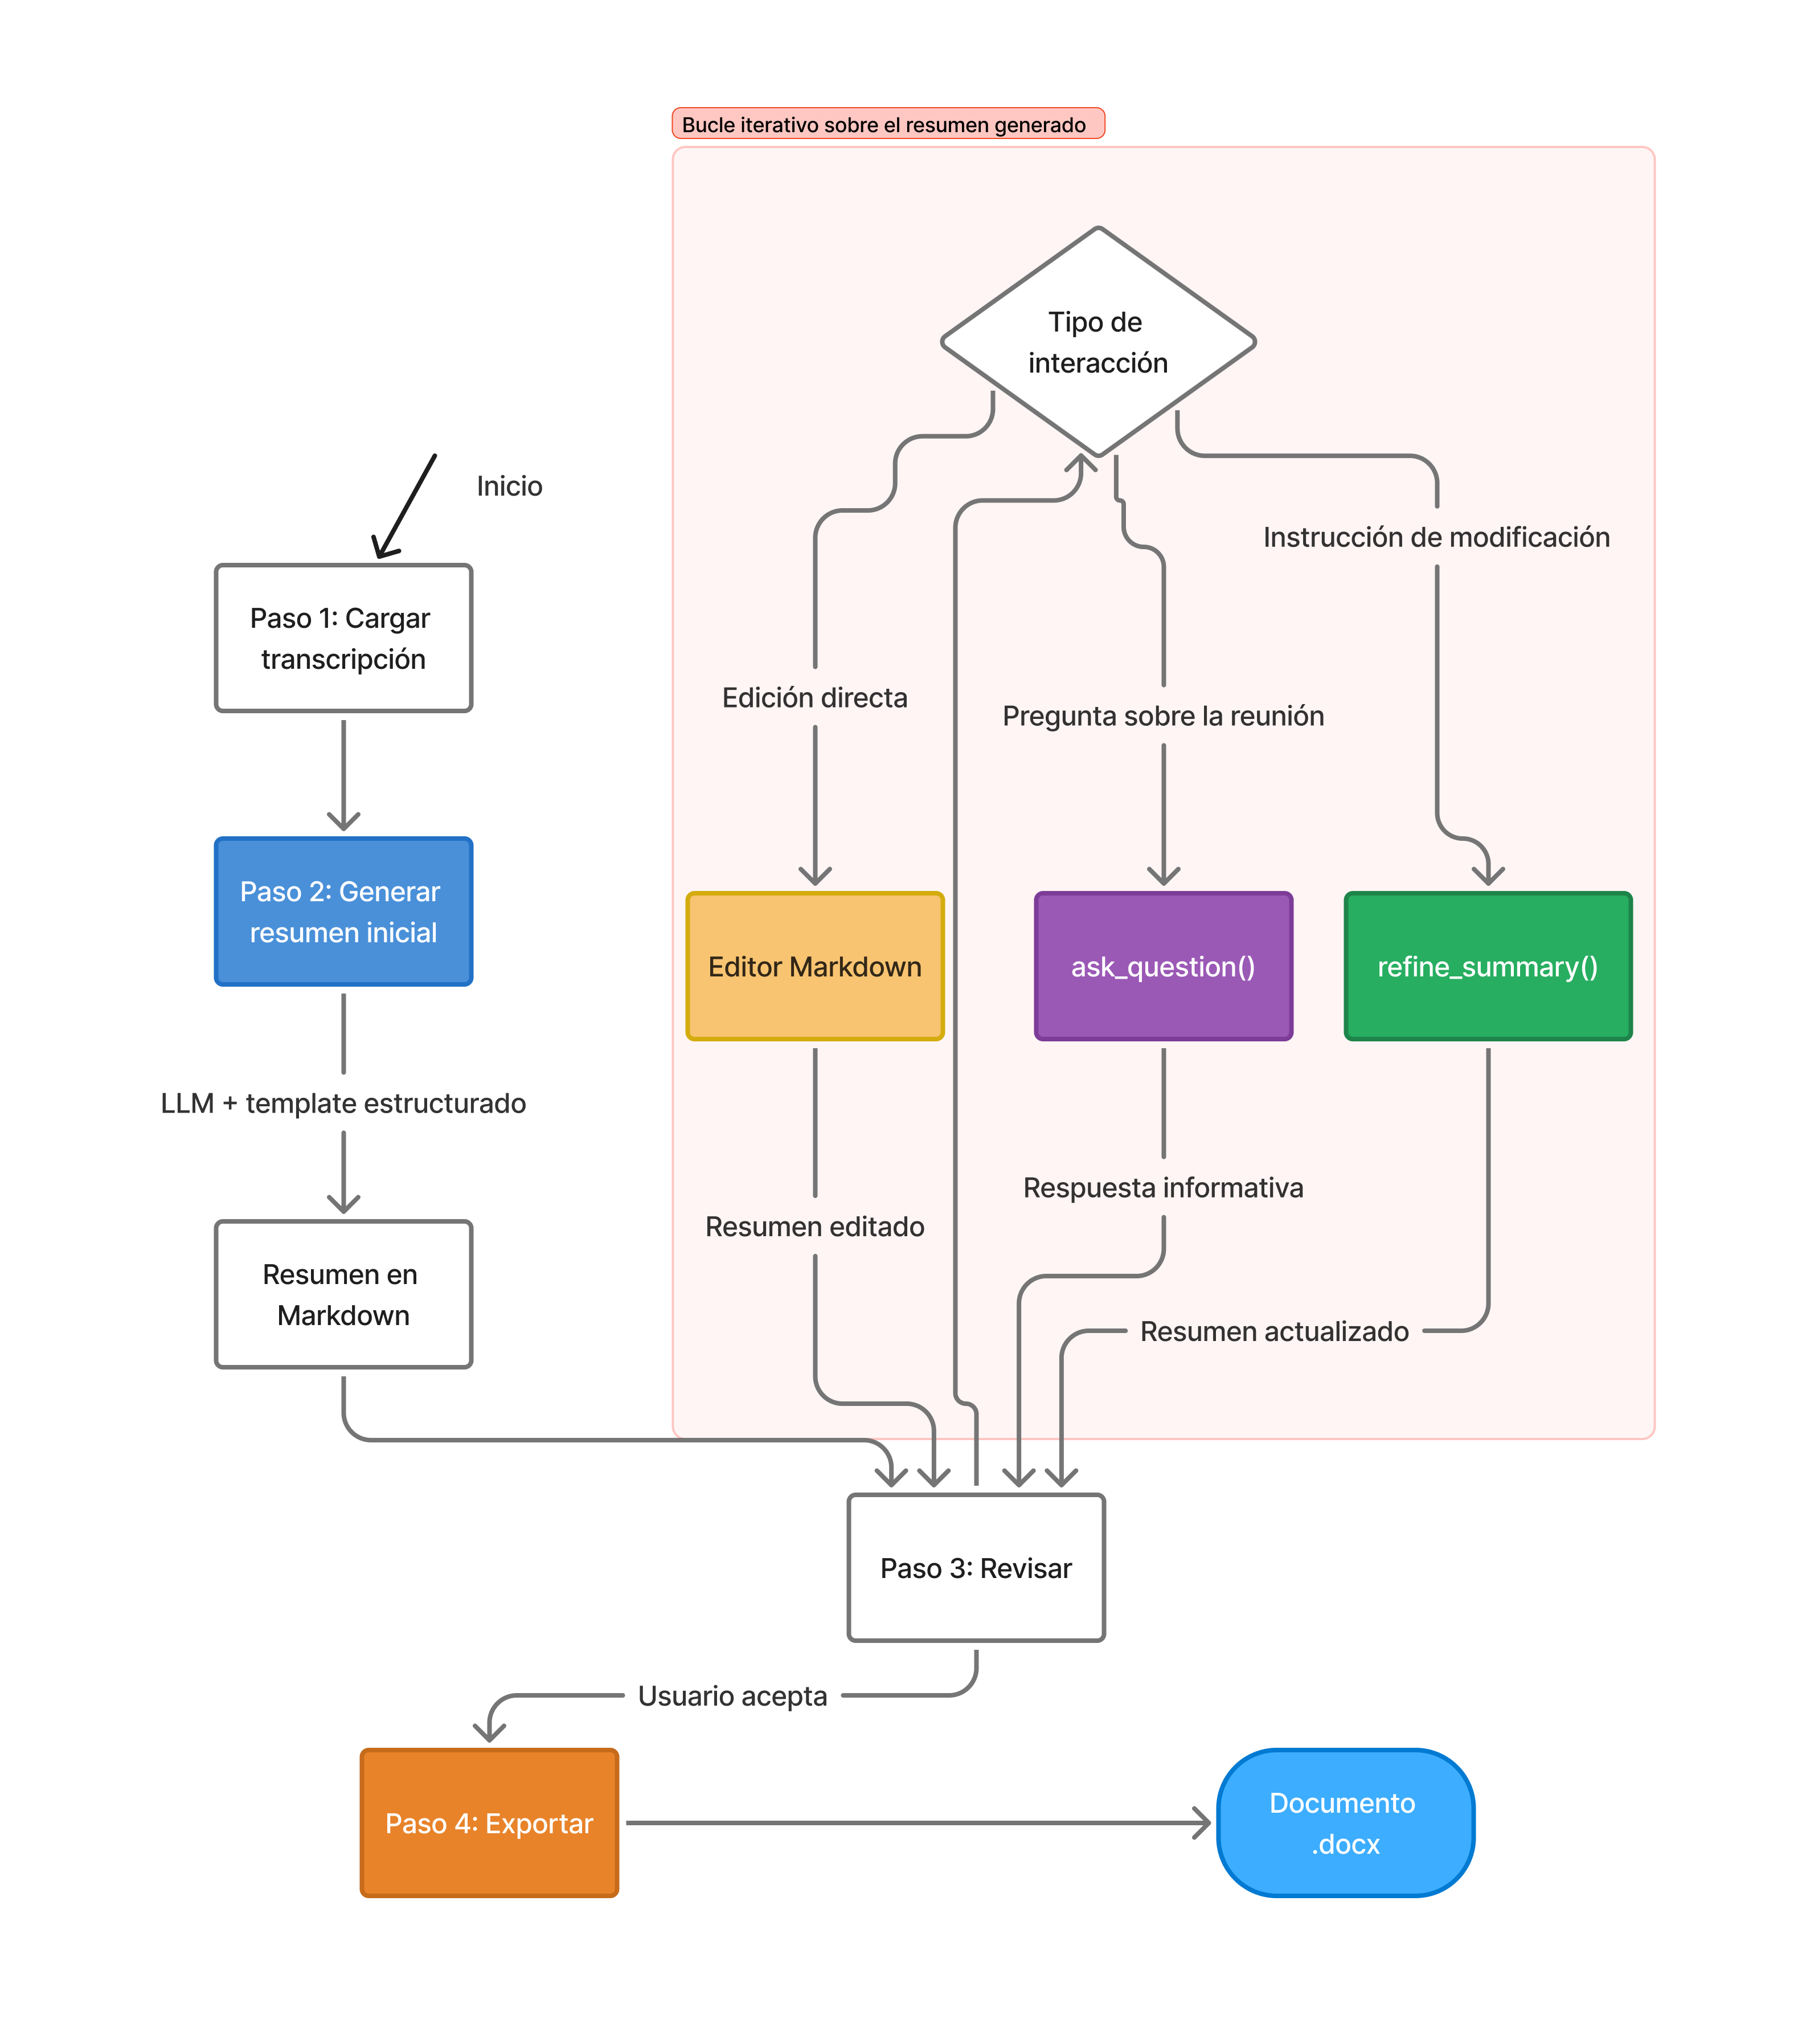
\includegraphics[width=0.6\textwidth]{imagenes/SeguimientDelCliente.png}
    \caption{Flujo de la implementación propia del módulo de seguimiento del cliente: generación del resumen inicial y bucle iterativo de refinamiento con \textit{Human in the Loop}. Generación propia.}
    \label{fig:seguimiento_cliente}
\end{figure}

\newpage

\section{Spec Driven Development: Implementación}
\label{sec:sdd_implementacion}
Una vez definidos los requerimientos iniciales del proyecto, el siguiente paso es garantizar que el desarrollo de código siga un flujo estructurado y trazable. Este capítulo describe la arquitectura de herramientas y asistentes que se ha configurado para implementar la metodología SDD en el día a día del equipo de desarrollo.

\subsection{Asistentes de Programación}
\label{sec:asistentes_programacion}
Una de las decisiones de diseño fundamentales del sistema es el rechazo a la dependencia exclusiva de un único proveedor de asistencia al código, fenómeno conocido como vendor lock-in. Para mitigar este riesgo, identificado ya en la planificación inicial (Riesgo~\ref{sec:riesgo2}), se ha optado por la integración de dos asistentes de programación de tipo CLI (\textit{Command-Line Interface}) que operan directamente desde la terminal:

\subsubsection{ClaudeCode}
\label{sec:claudecode}
ClaudeCode es la herramienta de asistencia a la programación desarrollada por Anthropic \cite{claude_code_2024}. Se trata de un agente CLI que opera directamente en la terminal del desarrollador, con acceso nativo al sistema de archivos del proyecto. ClaudeCode ha establecido el estándar actual en el ámbito de los agentes de programación, introduciendo o popularizando conceptos clave como los agentes especializados, los hooks de ciclo de vida, las skills, los plugins y el protocolo MCP (Model Context Protocol). Al tratarse de un servicio de pago, su uso está sujeto a las condiciones y tarifas de Anthropic.

\subsubsection{OpenCode}
\label{sec:opencode}
OpenCode \cite{opencode_2025} es un asistente de programación de código abierto compatible con modelos de lenguaje locales y remotos. Su arquitectura es funcionalmente equivalente a la de ClaudeCode: opera desde la terminal, tiene acceso al sistema de archivos y es compatible con el protocolo MCP, lo que lo hace interoperable con la mayoría de las herramientas y plugins desarrollados para el ecosistema. Su naturaleza open source y su compatibilidad con modelos locales lo convierten en la alternativa directa a ClaudeCode en escenarios donde se requiere control total sobre los costes o la privacidad de los datos.

\subsubsection{Justificación de la doble integración}
\label{sec:justificacion_doble_integracion}
La utilización de ambas herramientas no es redundante, sino estratégica. Al configurar el sistema de modo que ambos asistentes sean capaces de operar con la misma configuración de proyecto (archivos de instrucciones, plugins y MCPs), se elimina la dependencia de cualquiera de los dos proveedores. Si las condiciones de uno de ellos cambian de forma desfavorable, el equipo puede migrar su flujo de trabajo sin necesidad de reconfigurarlo desde cero.

Adicionalmente, los asistentes de tipo CLI resuelven de forma más limpia los problemas de integración con el entorno de desarrollo que afectan a los asistentes integrados en el IDE, ya que disponen de herramientas de edición, lectura y búsqueda implementadas directamente sobre el sistema de archivos del sistema operativo.

\subsubsection{Arquitectura interna: el patrón ReAct y su implementación en TypeScript}
\label{sec:react_pattern}
Para comprender plenamente cómo se pueden extender y configurar estas herramientas, es conveniente conocer la arquitectura interna sobre la que están construidas. Tanto ClaudeCode como OpenCode son aplicaciones de TypeScript que implementan un bucle de agente basado en el patrón ReAct (Reasoning + Acting), propuesto por Yao et al. (2022) \cite{yao_react_2023} como paradigma estándar para la construcción de agentes basados en modelos de lenguaje.

El patrón ReAct estructura el comportamiento del agente en un ciclo iterativo de tres fases:

\textbf{Razonamiento (Thought):} El modelo recibe el estado actual del contexto y genera un razonamiento interno en el que planifica el siguiente paso. Este razonamiento no es visible para el usuario, pero es el mecanismo por el que el agente decide qué acción tomar.

\textbf{Acción (Action):} El modelo emite una llamada a herramienta estructurada (\textit{tool call}) en formato JSON, especificando qué herramienta invocar y con qué parámetros. Las herramientas disponibles incluyen la lectura de archivos, la escritura de código y la ejecución de comandos en terminal.

\textbf{Observación (Observation):} El runtime de TypeScript ejecuta la acción sobre el sistema de archivos de la terminal y devuelve el resultado al modelo como nuevo mensaje en el historial. Este resultado se convierte en la entrada del siguiente ciclo.

\begin{figure}[H]
    \centering
    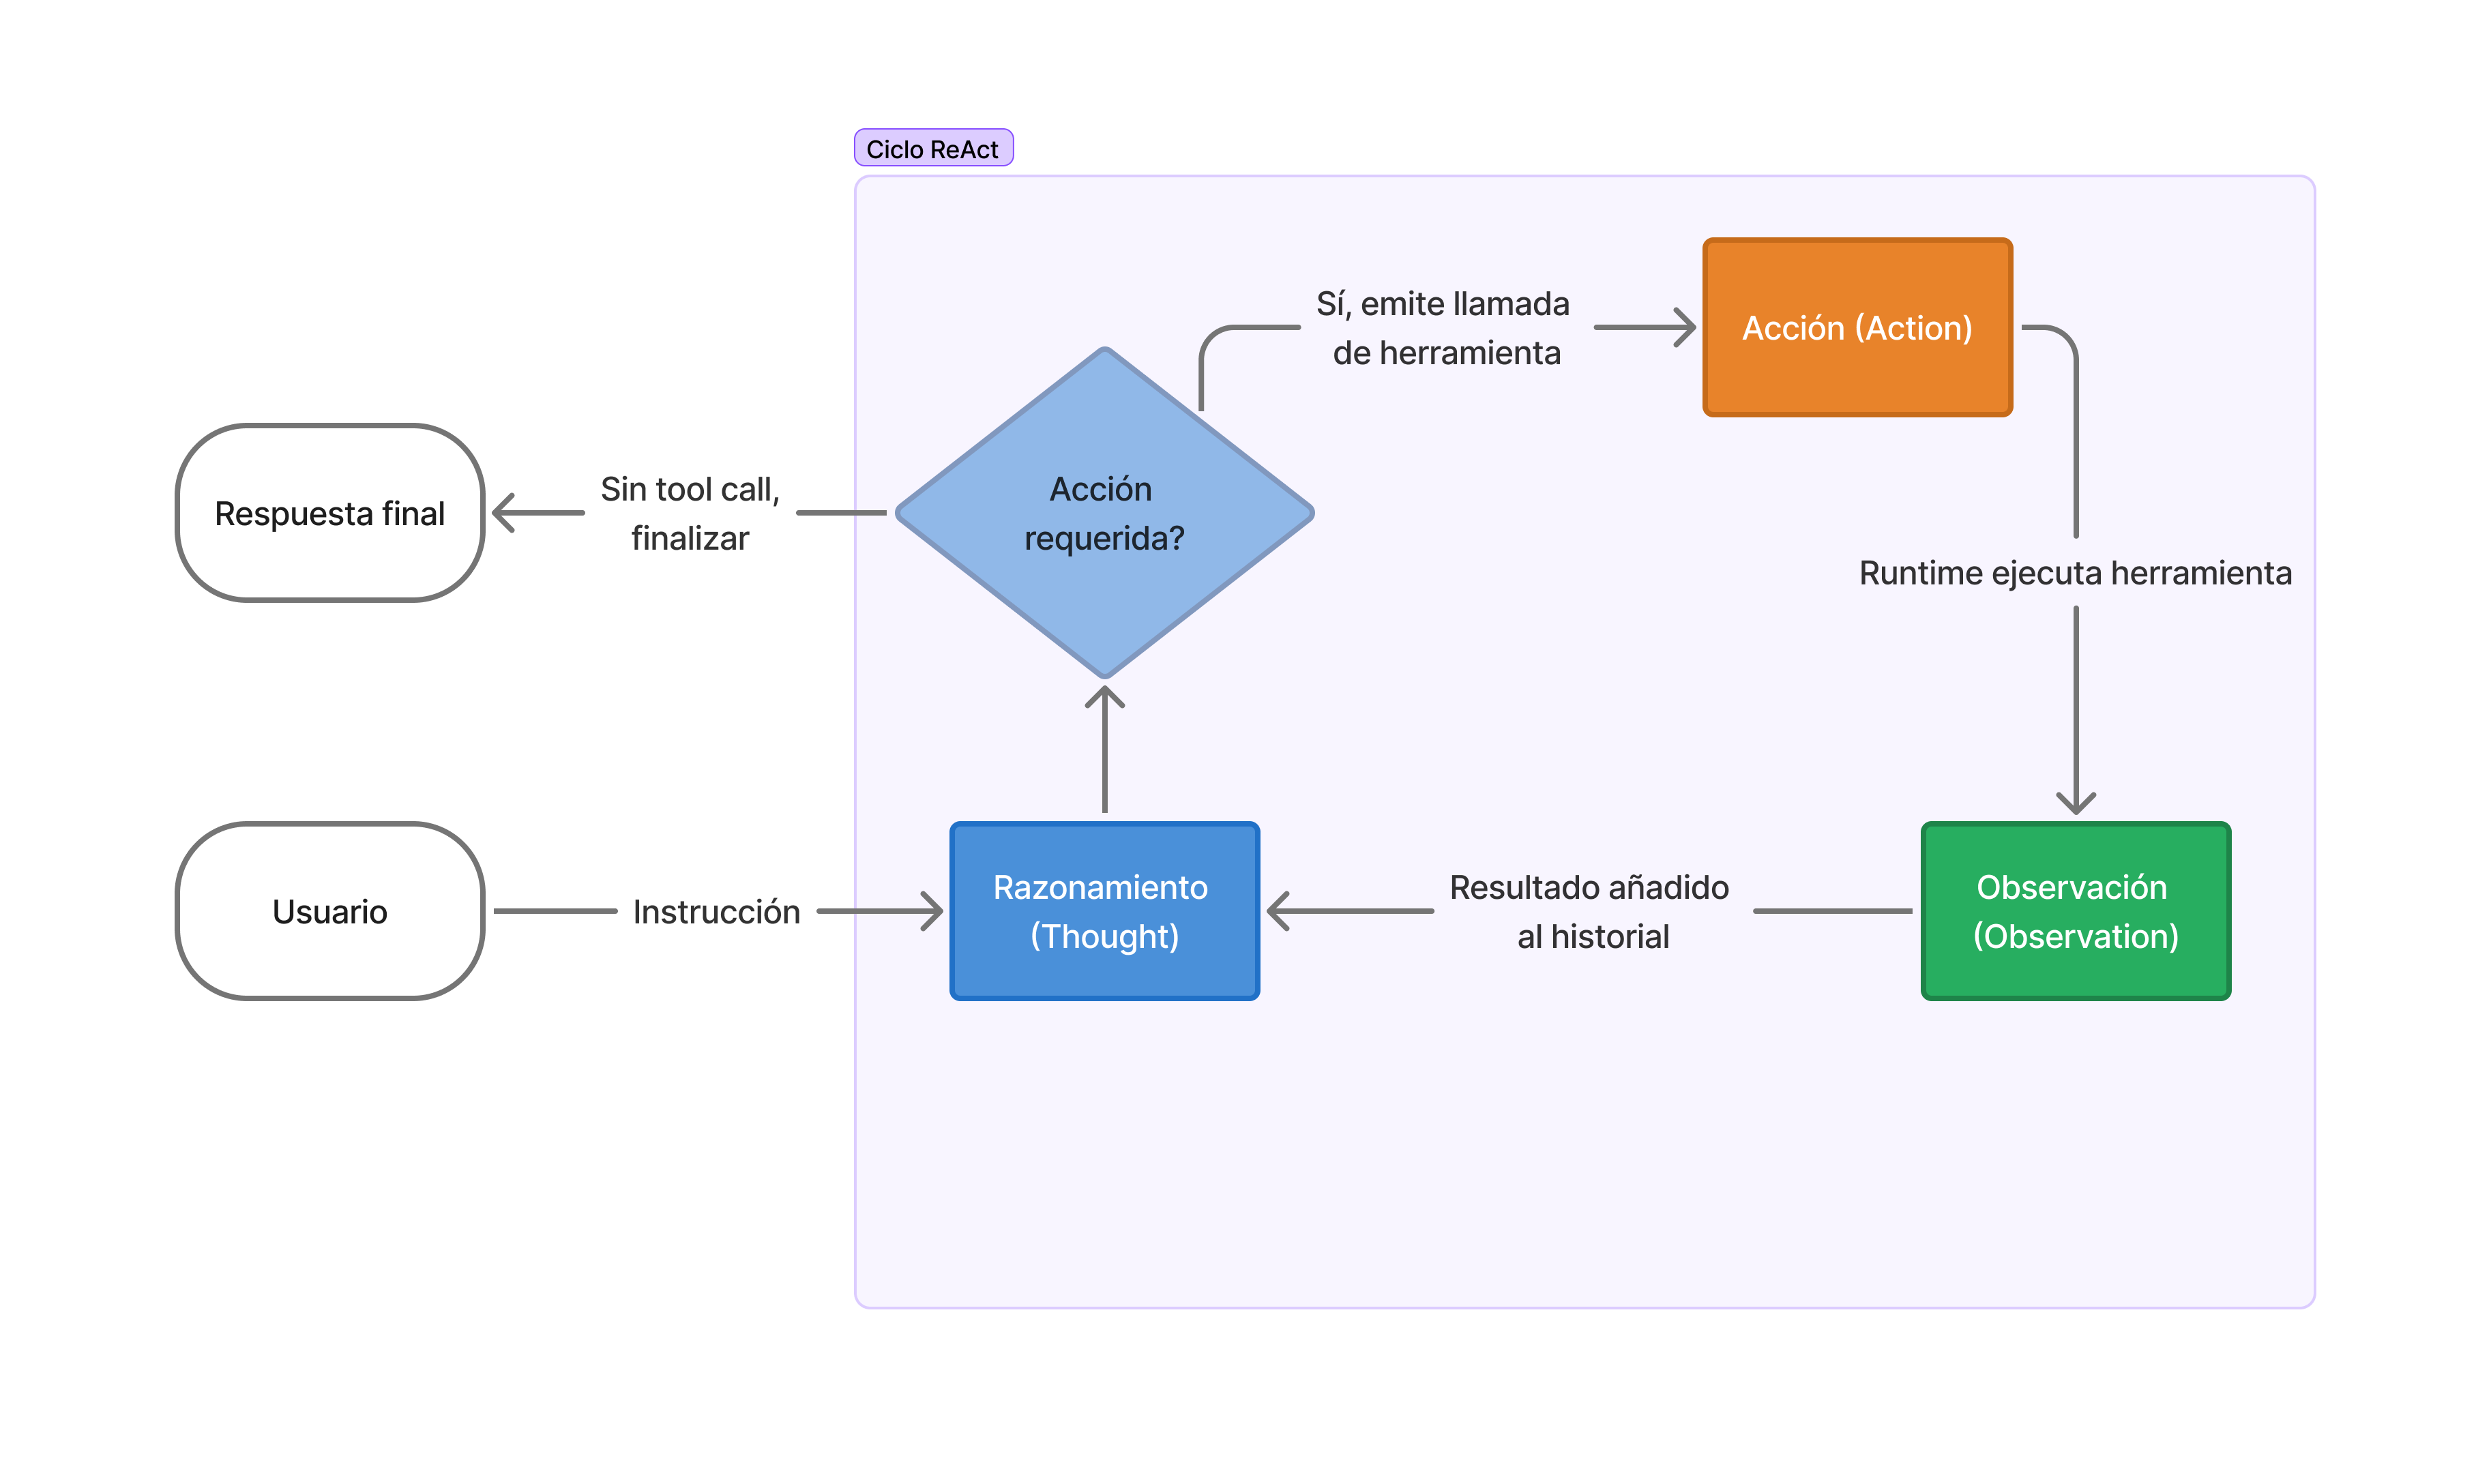
\includegraphics[width=0.85\textwidth]{imagenes/Ciclo_ReAct.png}
    \caption{Ciclo iterativo ReAct: el agente alterna entre Razonamiento, Acción y Observación hasta que no hay más herramientas que invocar. Generación propia.}
    \label{fig:ciclo_react}
\end{figure}

El runtime que orquesta este bucle está implementado en TypeScript sobre Node.js. Su flujo de ejecución puede describirse de forma simplificada en tres pasos:

\begin{enumerate}
    \item Al iniciarse una sesión, el runtime construye el system prompt combinando las instrucciones globales del asistente con el contenido del archivo de configuración del proyecto (CLAUDE.md o equivalente), y define el conjunto de herramientas disponibles mediante un esquema JSON.
    \item En cada iteración del bucle, el runtime envía el historial de conversación actualizado a la API del modelo. Si la respuesta contiene llamadas a herramienta, las ejecuta secuencialmente, añade los resultados al historial y lanza una nueva iteración.
    \item Si la respuesta no contiene llamadas a herramienta, el runtime la presenta al usuario como respuesta final y espera una nueva instrucción, reiniciando el ciclo con el historial acumulado.
\end{enumerate}

Este diseño en TypeScript es la base sobre la que se apoyan todos los mecanismos de extensibilidad descritos en las secciones siguientes: al tratarse de un proceso Node.js estándar, es posible interceptar el bucle en distintos puntos mediante hooks, inyectar herramientas adicionales mediante plugins, y conectar servicios externos mediante el protocolo MCP.

\subsection{Mecanismos de extensibilidad}
\label{sec:mecanismos_extensibilidad}
El valor diferencial de los asistentes CLI frente a otras soluciones reside en su arquitectura de extensibilidad. Antes de describir la configuración concreta del sistema, es necesario definir con precisión los conceptos que la componen, ya que estos términos ---plugin, MCP, hook, skill, agente--- se utilizan con frecuencia de forma imprecisa en la literatura del sector.

\subsubsection{Conceptos clave}
\label{sec:conceptos_clave_ext}
\begin{table}[H]
\centering
\begin{tabular}{p{2.5cm} p{8cm} p{5.5cm}}
\toprule
\textbf{Concepto} & \textbf{Qué es} & \textbf{Cuándo actúa} \\
\midrule
\textbf{Hook} & Callback registrado en el runtime que se ejecuta automáticamente ante eventos del ciclo de vida del agente (SessionStart, PreToolUse, PostToolUse, etc.). Permite inyectar comportamiento sin intervención explícita del usuario. & Al inicio de sesión, antes o después de editar archivos, o al ejecutar comandos de terminal. \\
\textbf{Skill} & Documento Markdown con instrucciones procedimentales especializadas para el agente, análogo a las skills de Claude Cowork (véase Fig.~\ref{fig:skill_definition}). Puede incluir scripts, templates y referencias a herramientas. & Cuando el agente detecta que una tarea requiere un procedimiento específico; el contenido se carga bajo demanda para no consumir tokens innecesariamente. \\
\textbf{Agente (subagente)} & Instancia del LLM creada dinámicamente por el orquestador para ejecutar una tarea en aislamiento, sin acceso al historial de conversación del orquestador. & Para tareas que requieren un contexto acotado e independiente, eliminando interferencias con el hilo principal. \\
\textbf{Plugin} & Paquete instalable (análogo a un paquete npm) que agrupa y distribuye skills, hooks, comandos y agentes. Es la unidad de distribución del ecosistema. Su estructura incluye carpetas \texttt{skills/}, \texttt{agents/} y un fichero \texttt{hooks.json}. & Al inicializar el proyecto; instalable a nivel de usuario o de proyecto con un único comando. \\
\textbf{MCP (Model Context Protocol)} & Protocolo estándar abierto que define cómo un proceso externo expone herramientas invocables al agente. El servidor MCP es un proceso independiente (en cualquier lenguaje) que ejecuta las operaciones y devuelve los resultados al runtime. & Cuando el agente necesita capacidades externas: consultar un grafo de código, buscar en la web, leer una base de datos, etc. \\
\bottomrule
\end{tabular}
\caption{Conceptos clave del sistema de extensibilidad de los asistentes CLI. Elaboración propia.}
\label{tab:conceptos_extensibilidad}
\end{table}

\textbf{Distinción entre MCP y Skill.} Aunque ambos mecanismos amplían las capacidades del agente, su naturaleza es diferente. Una skill es esencialmente un prompt procedimental: incluye instrucciones detalladas sobre cómo abordar una tarea y puede invocar herramientas locales durante su ejecución. Un servidor MCP, en cambio, expone herramientas atómicas acompañadas únicamente de una descripción de su interfaz, sin lógica de orquestación; la ejecución se produce en el proceso del servidor MCP, no en el runtime local del asistente. En la práctica, las skills definen \textit{cómo} debe razonar el agente ante una clase de tarea, mientras que los MCPs definen \textit{qué} operaciones externas puede invocar.

\newpage

\subsubsection{El ciclo de vida completo de una sesión en OpenCode}
\label{sec:ciclo_vida_opencode}
Para extender y configurar OpenCode de forma eficaz, es necesario comprender con exactitud en qué momento del ciclo se carga cada componente ---plugins, skills, herramientas y agentes--- y cómo interactúan durante una conversación. Aprovechando que opencode es una herramienta de código abierto, a continuación vamos a describir el ciclo de funcionamiento de forma detallada, desde la inicialización del proceso hasta la entrega de la respuesta al usuario.

\begin{figure}[H]
    \centering
    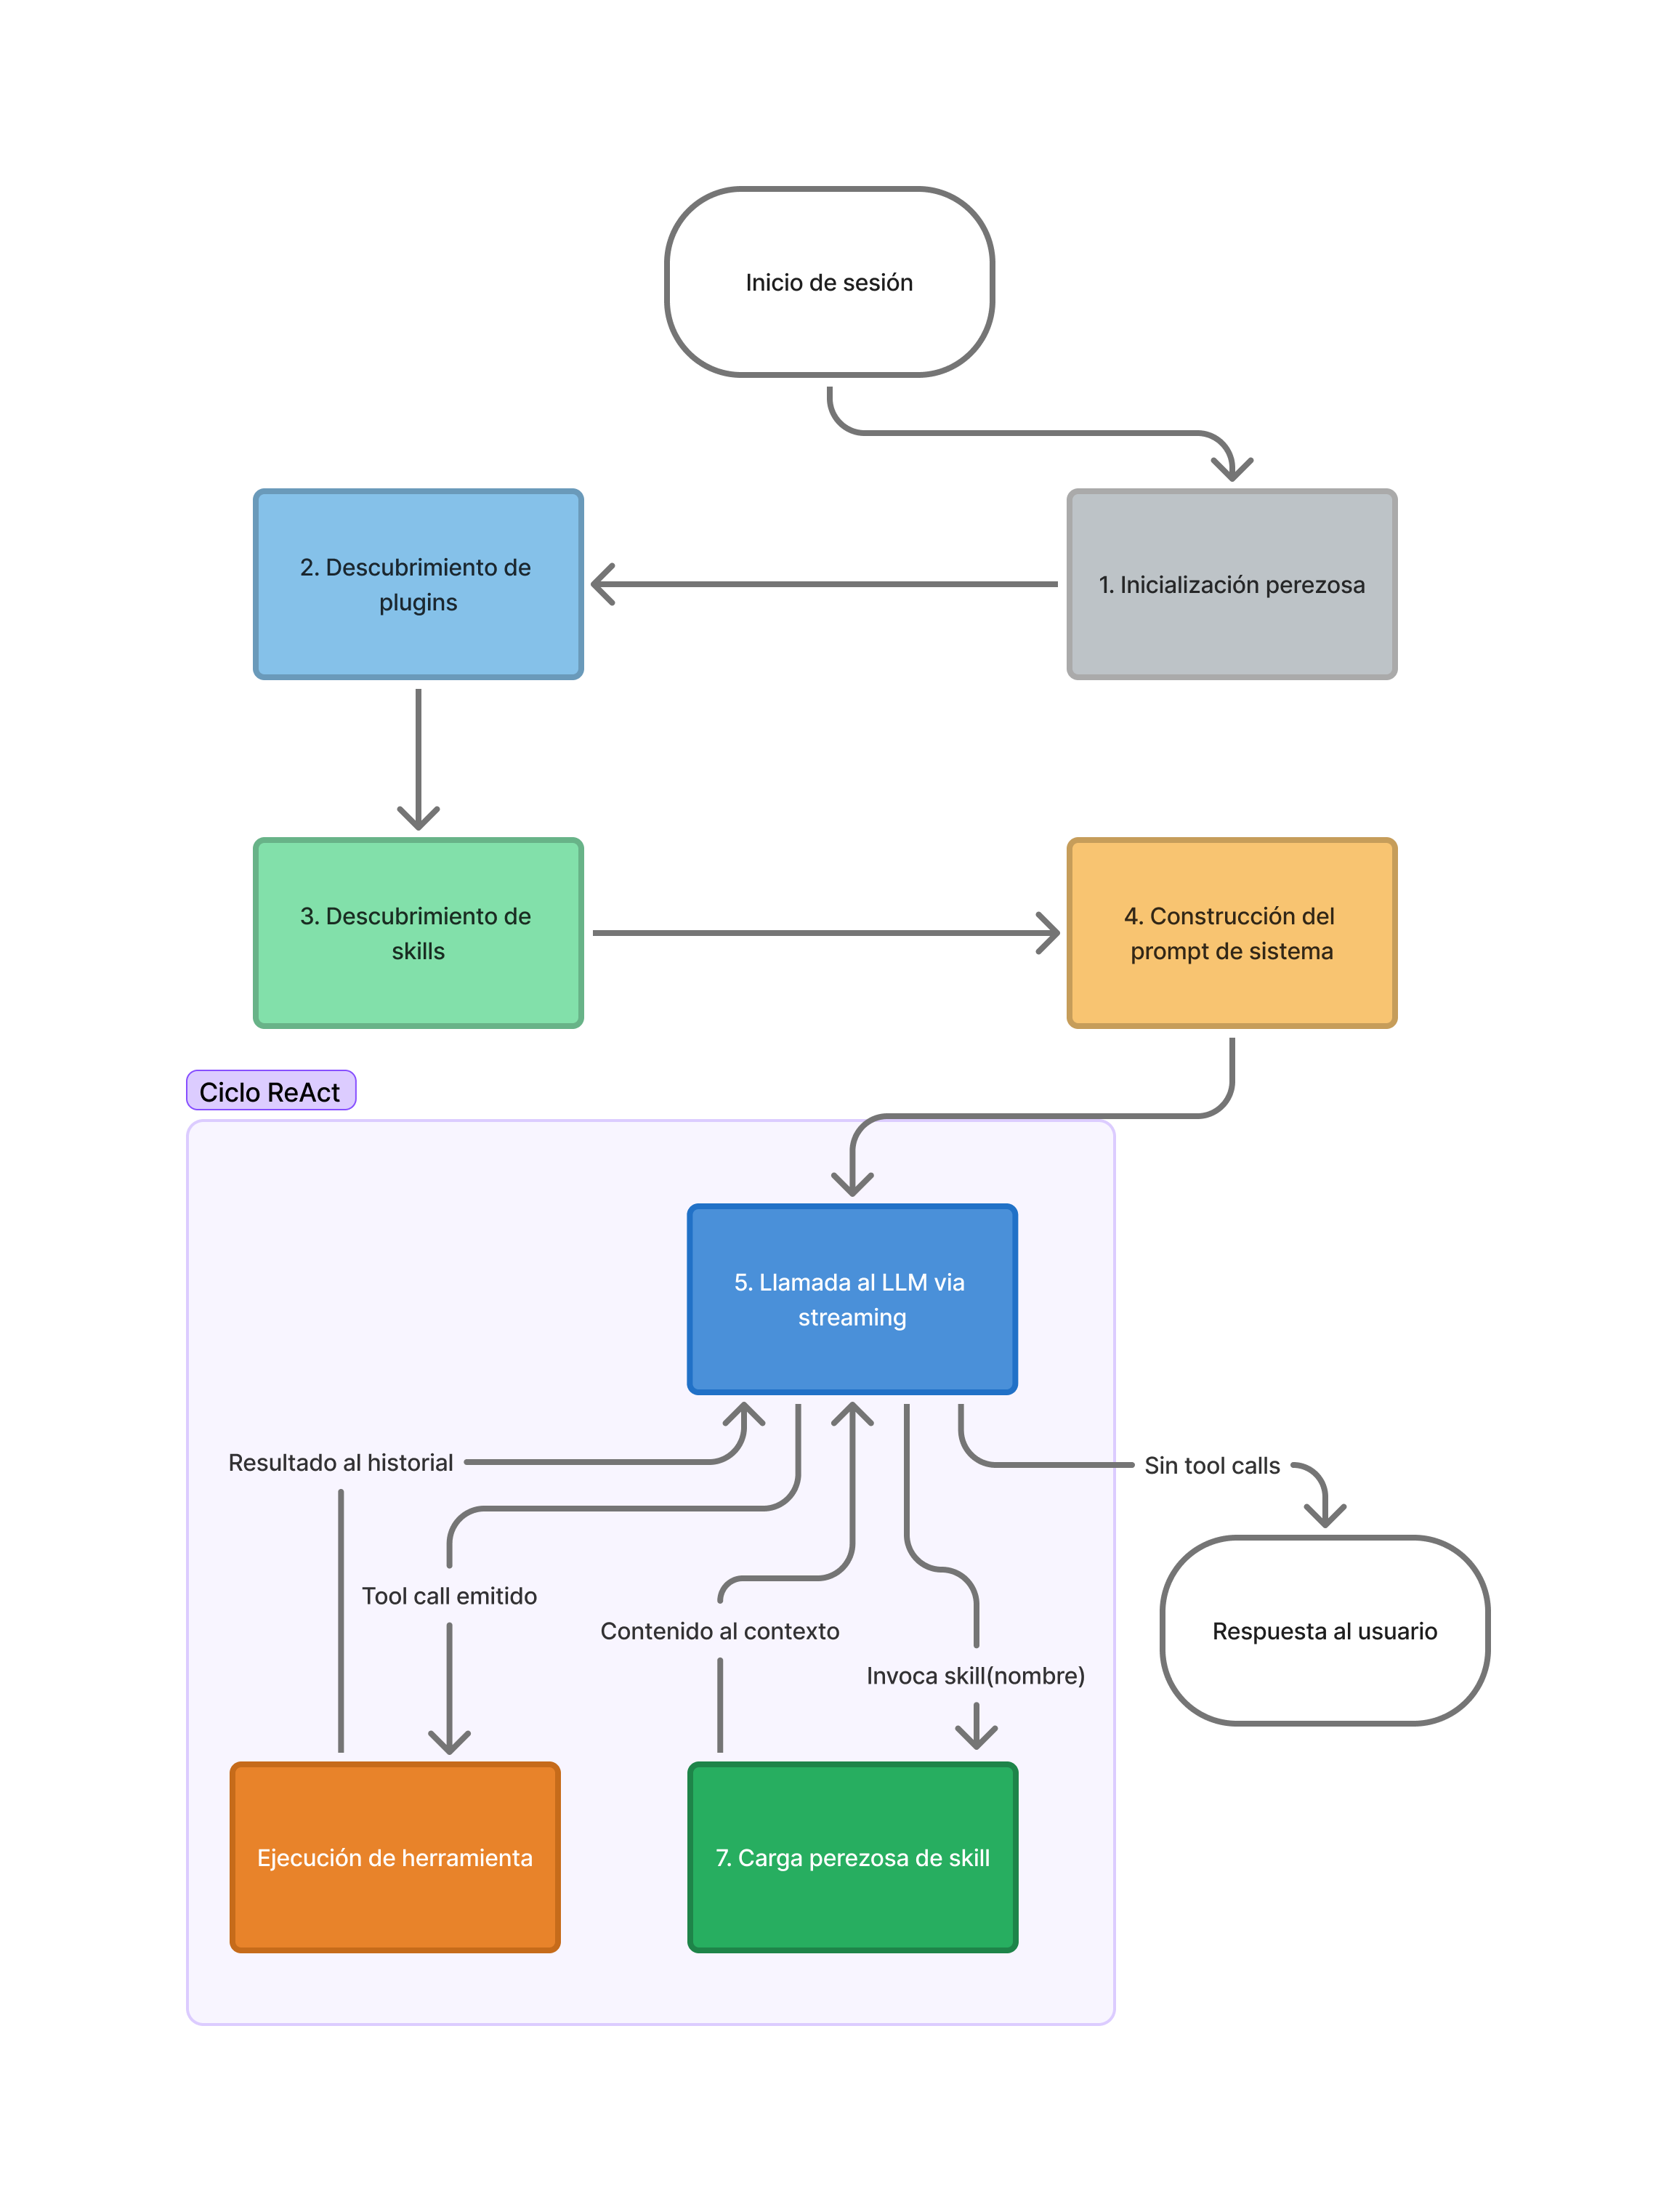
\includegraphics[width=0.7\textwidth]{imagenes/CicloSesiónOpenCode.png}
    \caption{Ciclo de vida completo de una sesión en OpenCode: desde la inicialización perezosa hasta la entrega de la respuesta, con el ciclo ReAct en el núcleo del bucle conversacional. Generación propia.}
    \label{fig:ciclo_sesion_opencode}
\end{figure}

\paragraph{Inicialización perezosa del espacio de trabajo.}
OpenCode implementa el patrón de inicialización perezosa (\textit{lazy initialization}): cuando el usuario abre un proyecto por primera vez en la sesión, el sistema no instancia de inmediato todos los servicios. Los plugins, el registro de herramientas, el catálogo de skills y los clientes MCP se crean la primera vez que son necesarios y se mantienen en caché para el resto de la sesión. Esto permite que el proceso arranque rápidamente con independencia del tamaño del proyecto.

\paragraph{Descubrimiento de plugins y herramientas.}
Cuando el registro de herramientas se inicializa por primera vez, OpenCode ejecuta el proceso de descubrimiento de plugins. Los plugins se cargan desde dos fuentes: (1) los plugins internos del propio asistente, integrados directamente en el binario (autenticación con Codex, GitHub Copilot, GitLab, Cloudflare y otros), y (2) los plugins externos declarados explícitamente en el archivo de configuración de OpenCode, que pueden ser paquetes npm instalados bajo demanda o rutas de archivo locales (por ejemplo, \texttt{./mi-plugin.ts}). OpenCode no escanea automáticamente los directorios del proyecto en busca de plugins; la declaración explícita en la configuración es requisito indispensable para cargar un plugin externo. Cada plugin puede registrar herramientas adicionales mediante la interfaz de hooks que OpenCode expone, concretamente el campo \texttt{Hooks.tool}. Todas las herramientas ---las nativas del asistente más las aportadas por plugins y por los servidores MCP configurados--- se registran en el registro global y se describen al modelo mediante un esquema JSON.

\paragraph{Descubrimiento de skills.}
Paralelamente al descubrimiento de plugins, el sistema escanea el sistema de archivos para localizar las skills disponibles. La búsqueda se realiza en un conjunto predefinido de rutas: \texttt{\textasciitilde/.claude/skills/}, \texttt{\textasciitilde/.agents/skills/}, los directorios \texttt{.claude/} y \texttt{.agents/} de la raíz del proyecto, los directorios de configuración global de OpenCode, y las rutas adicionales declaradas en el campo \texttt{skills.paths} del archivo \texttt{opencode.json}. Para cada skill encontrada, el sistema registra su nombre, descripción y ubicación. Sin embargo, el contenido completo de la skill \textit{no} se carga en este momento: el descubrimiento construye únicamente el catálogo, sin consumir tokens del contexto.

\paragraph{Construcción del system prompt.}
Al recibir un mensaje del usuario, el sistema construye el system prompt que se enviará al LLM combinando cuatro componentes:
\begin{enumerate}
    \item \textbf{Prompt base del proveedor}: instrucciones genéricas del asistente, adaptadas al modelo concreto que esté activo (Anthropic Claude, Google Gemini u otros). Si el agente activo define un campo \texttt{prompt} propio en su configuración, este sustituye al prompt base del proveedor.
    \item \textbf{Entorno y contexto}: directorio de trabajo actual, fecha, plataforma del sistema operativo y agente activo en la sesión.
    \item \textbf{Catálogo de skills}: una sección del system prompt lista los nombres y descripciones breves de todas las skills descubiertas. Esta lista es lo único que el LLM recibe sobre las skills en el prompt inicial; el contenido detallado de cada skill se carga bajo demanda más adelante.
    \label{concepto:archivo_instrucciones}
    \item \textbf{Archivo de instrucciones del proyecto}: el contenido de un archivo de instrucciones del repositorio con el nombre \texttt{AGENTS.md} o  \texttt{CLAUDE.md} (para asegurar compatibilidad con proyectos desarrollados usando ClaudeCode) , que típicamente incluye la descripción del proyecto, el stack tecnológico, los estándares de código del equipo y las restricciones que el agente debe respetar. Además, los plugins pueden modificar el system prompt resultante mediante el hook \texttt{experimental.chat.system.transform}, inyectando secciones adicionales antes de que el prompt se envíe al modelo.
\end{enumerate}

\paragraph{La llamada al LLM mediante streaming.}
Una vez construido el system prompt y serializado el historial de conversación, OpenCode realiza la llamada al modelo a través de la función \texttt{streamText()} del SDK de Vercel AI. Esta función gestiona la transmisión de tokens en tiempo real (\textit{streaming}), de modo que el agente puede reaccionar a cada fragmento de texto generado por el modelo sin esperar a que la respuesta esté completa. Antes de la llamada, los hooks \texttt{chat.params} y \texttt{chat.headers} permiten a los plugins inyectar parámetros adicionales (temperatura, cabeceras HTTP, etc.).

La respuesta del modelo llega como un flujo asíncrono de eventos que el runtime consume uno a uno. Los tipos de eventos posibles incluyen: inicio de paso, fragmentos de texto, razonamiento interno del modelo, llamadas a herramienta, resultados de herramienta y señales de finalización. A medida que se reciben fragmentos de texto, estos se propagan a la interfaz de usuario en tiempo real, lo que permite al desarrollador seguir el razonamiento del agente sin esperar a que la respuesta esté completa.

\paragraph{Ejecución de herramientas.}
Cuando el modelo decide invocar una herramienta, el runtime recibe el evento correspondiente con el nombre de la herramienta y sus parámetros. Antes de ejecutar la herramienta, se disparan los hooks \texttt{tool.execute.before} de todos los plugins registrados; tras la ejecución, se disparan los hooks \texttt{tool.execute.after}. El resultado se añade al historial de conversación como un nuevo mensaje de tipo \textit{tool result} y se inicia un nuevo ciclo del bucle ReAct, reenviando el historial actualizado al modelo.

\paragraph{Carga perezosa de skills bajo demanda.}
La herramienta \texttt{skill} ilustra con claridad el principio de carga perezosa. Cuando el modelo, al ver el catálogo de skills en el system prompt, decide que necesita las instrucciones de una skill concreta para ejecutar una tarea, invoca la herramienta \texttt{skill} con el nombre de la skill como parámetro. Es en ese momento ---y solo en ese momento--- cuando el sistema lee el archivo \texttt{SKILL.md} correspondiente del disco, enumera los ficheros asociados a la skill (hasta un máximo de diez), y devuelve el contenido completo al modelo envuelto en una etiqueta XML estructurada. De esta forma, el contenido detallado de las skills no ocupa tokens del contexto inicial: solo las descripciones breves del catálogo están siempre presentes; los contenidos completos se cargan únicamente cuando el modelo los solicita. La skill \textit{using-colbPowers} de colbPowers es una excepción deliberada a este principio: al inyectarse mediante el hook SessionStart antes de que comience la conversación, su contenido completo llega al modelo directamente en el system prompt, sin pasar por el mecanismo de carga perezosa. Esto garantiza que las reglas de orquestación estén activas desde el primer mensaje, sin depender de que el modelo recuerde invocar la herramienta \texttt{skill}.

\paragraph{Similitud con ClaudeCode.}
ClaudeCode implementa un pipeline estructuralmente análogo en lo que respecta al ciclo de vida de la conversación. Aunque las implementaciones concretas difieren ---ClaudeCode no es software libre---, el flujo conceptual comparte los mismos patrones: inicialización perezosa de servicios al inicio de la sesión, construcción del system prompt a partir de archivos de instrucciones y catálogos de skills, bucle ReAct con llamadas a herramienta y streaming de tokens, carga perezosa de skills bajo demanda, y mecanismos de hooks para interceptar el ciclo de vida.

Sin embargo, existen diferencias arquitectónicas significativas que conviene señalar:

\begin{table}[H]
\centering
\begin{tabular}{p{2.8cm} p{4.5cm} p{7cm}}
\toprule
\textbf{Dimensión} & \textbf{ClaudeCode} & \textbf{OpenCode} \\
\midrule
\textbf{Proveedores LLM} & Exclusivo de Anthropic (modelos Claude) & Más de 25 proveedores a través del SDK de Vercel AI (OpenAI, Google, Azure, Bedrock, Mistral, Groq, GitHub Copilot, entre otros) \\
\textbf{Modelo de interfaz} & Exclusivamente CLI; interfaz renderizada en terminal mediante React e Ink & Servidor HTTP local (Hono) con aplicación web SolidJS; soporta además aplicaciones de escritorio nativas (Tauri y Electron) \\
\textbf{Persistencia} & Estado en memoria y ficheros JSON locales & Sesiones persistidas en SQLite con instantáneas del sistema de ficheros antes de cada invocación de herramienta, lo que permite revertir cambios \\
\textbf{Framework técnico} & TypeScript estándar para la composición de servicios & Uso intensivo del framework Effect (programación funcional monádica) para gestión de dependencias, errores y concurrencia \\
\bottomrule
\end{tabular}
\caption{Comparativa arquitectónica entre ClaudeCode y OpenCode. Elaboración propia.}
\label{tab:comparativa_asistentes}
\end{table}

Esta equivalencia a nivel de flujo de conversación ---y no de arquitectura completa--- es la que hace posible que un plugin como colbPowers, que se apoya en skills y hooks genéricos, funcione de forma comparable en ambos asistentes, si bien los adaptadores de hooks concretos difieren entre plataformas.

\subsubsection{Hooks de ciclo de vida}
\label{sec:hooks_ciclo_vida}
ClaudeCode expone un sistema de hooks configurables que permite registrar callbacks para distintos eventos del ciclo de vida del agente. Estos hooks pueden definirse de dos formas: directamente por el desarrollador en el archivo \texttt{settings.json} del proyecto o del usuario, o bien declararse dentro de un plugin mediante un archivo \texttt{hooks.json} incluido en el paquete del plugin ---que es el mecanismo que utiliza colbPowers. Los hooks más relevantes para el flujo SDD son \texttt{SessionStart} (inyección de contexto al inicio de sesión) y \texttt{PreToolUse} (intercepción antes de ejecutar una herramienta concreta, útil para forzar consultas al grafo de código antes de cualquier modificación). En OpenCode, estos hooks se implementan mediante callbacks definidos en el plugin JavaScript correspondiente, con semántica equivalente. En ambas plataformas, plugins y servidores MCP se instalan a nivel de proyecto o de usuario, lo que garantiza que el conjunto de herramientas y comportamientos esté disponible de forma consistente en todas las sesiones del equipo.

\subsubsection{Skills y agentes en colbPowers}
\label{sec:skills_agentes_colbpowers}
colbPowers hace un uso central de ambos mecanismos. Las skills definen el comportamiento del orquestador en cada fase del ciclo SDD: el skill \textit{using-colbpowers} (inyectado en SessionStart) contiene las reglas de orquestación y detección de estado del proyecto; \textit{brainstorming} y \textit{writing-plans} instruyen al agente sobre cómo producir los documentos de diseño y planificación; \textit{requesting-code-review} define el protocolo de auditoría del código generado. Los subagentes se crean dinámicamente cuando una tarea requiere ejecución aislada: el orquestador genera un prompt específico para esa tarea (incluyendo el design.md y el tasks.md relevantes, y excluyendo el resto del historial) y lanza un subagente que opera exclusivamente sobre ese contexto acotado.

\subsection{Herramientas de Apoyo al Flujo SDD}
\label{sec:herramientas_apoyo_sdd}
La efectividad del flujo SDD depende en gran medida de la calidad del contexto que el agente tiene disponible en cada momento. A continuación se describen las herramientas principales integradas en el sistema.

\subsubsection{code-review-graph}
\label{sec:code_review_graph}
code-review-graph \cite{code_review_graph_2025} es una herramienta de código abierto que utiliza el parser de sintaxis Tree-Sitter para analizar el repositorio y construir un grafo de dependencias entre las distintas entidades de código (funciones, clases, módulos). Este grafo se almacena en una base de datos SQLite local y se expone al agente a través de un servidor MCP, proporcionando un mecanismo eficiente para navegar la estructura del código sin necesidad de leer todos los archivos del proyecto.

La integración de esta herramienta aborda directamente el problema de gestión de la ventana de contexto identificado en el apartado de riesgos (sección~\ref{sec:riesgo5}). En pruebas preliminares realizadas sobre un monorepo de Colb.Ai, el agente con code-review-graph integrado necesitó aproximadamente 40.000 tokens para describir la arquitectura del proyecto, frente a los 64.000 tokens requeridos sin la herramienta, lo que supone una reducción del 37,5\verb|%| en esa prueba concreta. Las capacidades que expone al agente incluyen:
\begin{itemize}
    \item Análisis de diffs de git para identificar cambios de mayor riesgo.
    \item Cálculo del radio de impacto (\textit{blast radius}) de cualquier modificación.
    \item Identificación de los flujos de ejecución afectados por un cambio.
    \item Búsqueda semántica de entidades de código (funciones, clases, módulos).
    \item Obtención de una visión de alto nivel de la arquitectura del sistema.
\end{itemize}

\subsubsection{Herramientas de métricas de complejidad}
\label{sec:metricas_complejidad}
La disponibilidad del árbol sintáctico abstracto (AST) de Tree-Sitter en la base de code-review-graph permite calcular métricas de calidad de código de forma granular a nivel de función. Las métricas de interés son la Complejidad Ciclomática \cite{McCabe_Complexity} (número de caminos independientes en el flujo de control de una función), el Volumen de Halstead (medida del vocabulario del código basada en operadores y operandos únicos) y el Índice de Mantenibilidad \cite{oman_maintainability_1992} (combinación logarítmica de las dos métricas anteriores junto con las líneas de código). Estas métricas se calculan durante la fase de construcción del grafo y se almacenan como atributos de cada nodo, quedando disponibles para que el agente las consulte al auditar el código generado.

\subsubsection{colbPowers: flujo de trabajo}
\label{sec:colbpowers_flujo}
colbPowers \cite{colbpowers_2026} es un plugin desarrollado a partir de la base proporcionada por el plugin \verb|"|superpowers\verb|"| \cite{superpowers_2025}, colbPowers es instalable en cualquier proyecto y implementa el flujo de trabajo Spec-First de forma autónoma. Una vez instalado, no requiere que el desarrollador recuerde invocar comandos ni seguir un protocolo manual, gracias a una combinación de hooks que inyectan contexto y skills, el agente es capaz de entender la etapa del desarrollo en la que se encuentra en todo momento. 

Distribuir el sistema como un plugin ---en lugar de como un conjunto de archivos de skills copiados manualmente en el proyecto--- aporta dos garantías que los archivos por sí solos no pueden ofrecer: el hook \texttt{SessionStart}, que inyecta la skill de bootstrap de forma incondicional en cada sesión sin depender de que el desarrollador la invoque, y una instalación cómoda y reproducible en cualquier proyecto, ya que los plugins se referencian directamente desde su repositorio en GitHub y ambos asistentes los descargan e instalan automáticamente.

El diseño de colbPowers no es arbitrario: cada mecanismo de extensibilidad descrito en las secciones anteriores cumple un papel arquitectónico específico dentro del flujo SDD. El hook \texttt{SessionStart} convierte el flujo de trabajo de un protocolo opcional en un comportamiento por defecto: al inyectar las reglas de orquestación antes de que el modelo reciba el primer mensaje, garantiza que el agente no pueda operar sin tenerlas presentes, independientemente de si el desarrollador las invoca o no. Las skills codifican cada fase del ciclo SDD como un procedimiento especializado e independiente: al cargarse únicamente cuando son necesarias, la especificación de brainstorming no ocupa contexto durante la revisión de código, y viceversa, manteniendo el consumo de tokens acotado a la fase activa en cada momento. Los subagentes aislados protegen la integridad de la especificación frente a la deriva conversacional: al arrancar sin acceso al historial de la sesión principal, el subagente implementador solo puede basar sus decisiones en el \texttt{design.md} que el orquestador le proporciona explícitamente, eliminando el riesgo de que cambios de alcance discutidos informalmente en el chat contaminen la implementación. Finalmente, el propio skill \textit{using-colbPowers}, inyectado en cada arranque, instruye al agente a verificar que \texttt{constitution.md} y \texttt{features.md} existen antes de cualquier otra acción, y a crearlos interactivamente si no es así: la especificación no es un documento opcional que el desarrollador puede consultar, sino una precondición estructural al inicio de cada sesión.

\paragraph{Estructura del proyecto esperada}
Para funcionar, colbPowers asume que el proyecto dispone de una plantilla de repositorio con una estructura específica bajo el directorio \texttt{.specs/memory/}. Esta plantilla incluye los documentos base del proyecto y puede contener adicionalmente indicaciones de estilo, planificación, o apuntes y referencias de proyectos anteriores que sirven de contexto al agente:

\textbf{constitution.md:} Documento de alcance global. Define la visión del proyecto, el stack tecnológico, los estándares de código no negociables y las reglas de gobernanza. Es la fuente de verdad sobre cómo se trabaja en este proyecto.

\textbf{features.md:} Roadmap del producto. Lista todas las features aprobadas con su descripción, requisitos funcionales, restricciones técnicas y dependencias. Cualquier nueva funcionalidad debe estar aquí definida antes de poder planificarse.

En caso de que una de las anteriores no exista. Al agente se le indica que ejecute las skills de "defining-constitution" y "defining-features", para popular estos archivos a través de un proceso iteractivo de preguntas al usuario.

\textbf{docs/specs/:} Documentos de diseño por feature: descripción del comportamiento esperado, decisiones de arquitectura y justificación técnica de cada implementación.

\textbf{docs/plans/:} Planes de implementación granulares por feature: listas de tareas ordenadas con criterios de aceptación.



\paragraph{Flujo de trabajo autónomo}
El flujo de trabajo completo se desarrolla de la siguiente forma cuando el usuario solicita cualquier cambio o nueva funcionalidad:

% Metemos aquí la fotillo con el diagrama
\begin{figure}[H]
    \centering
    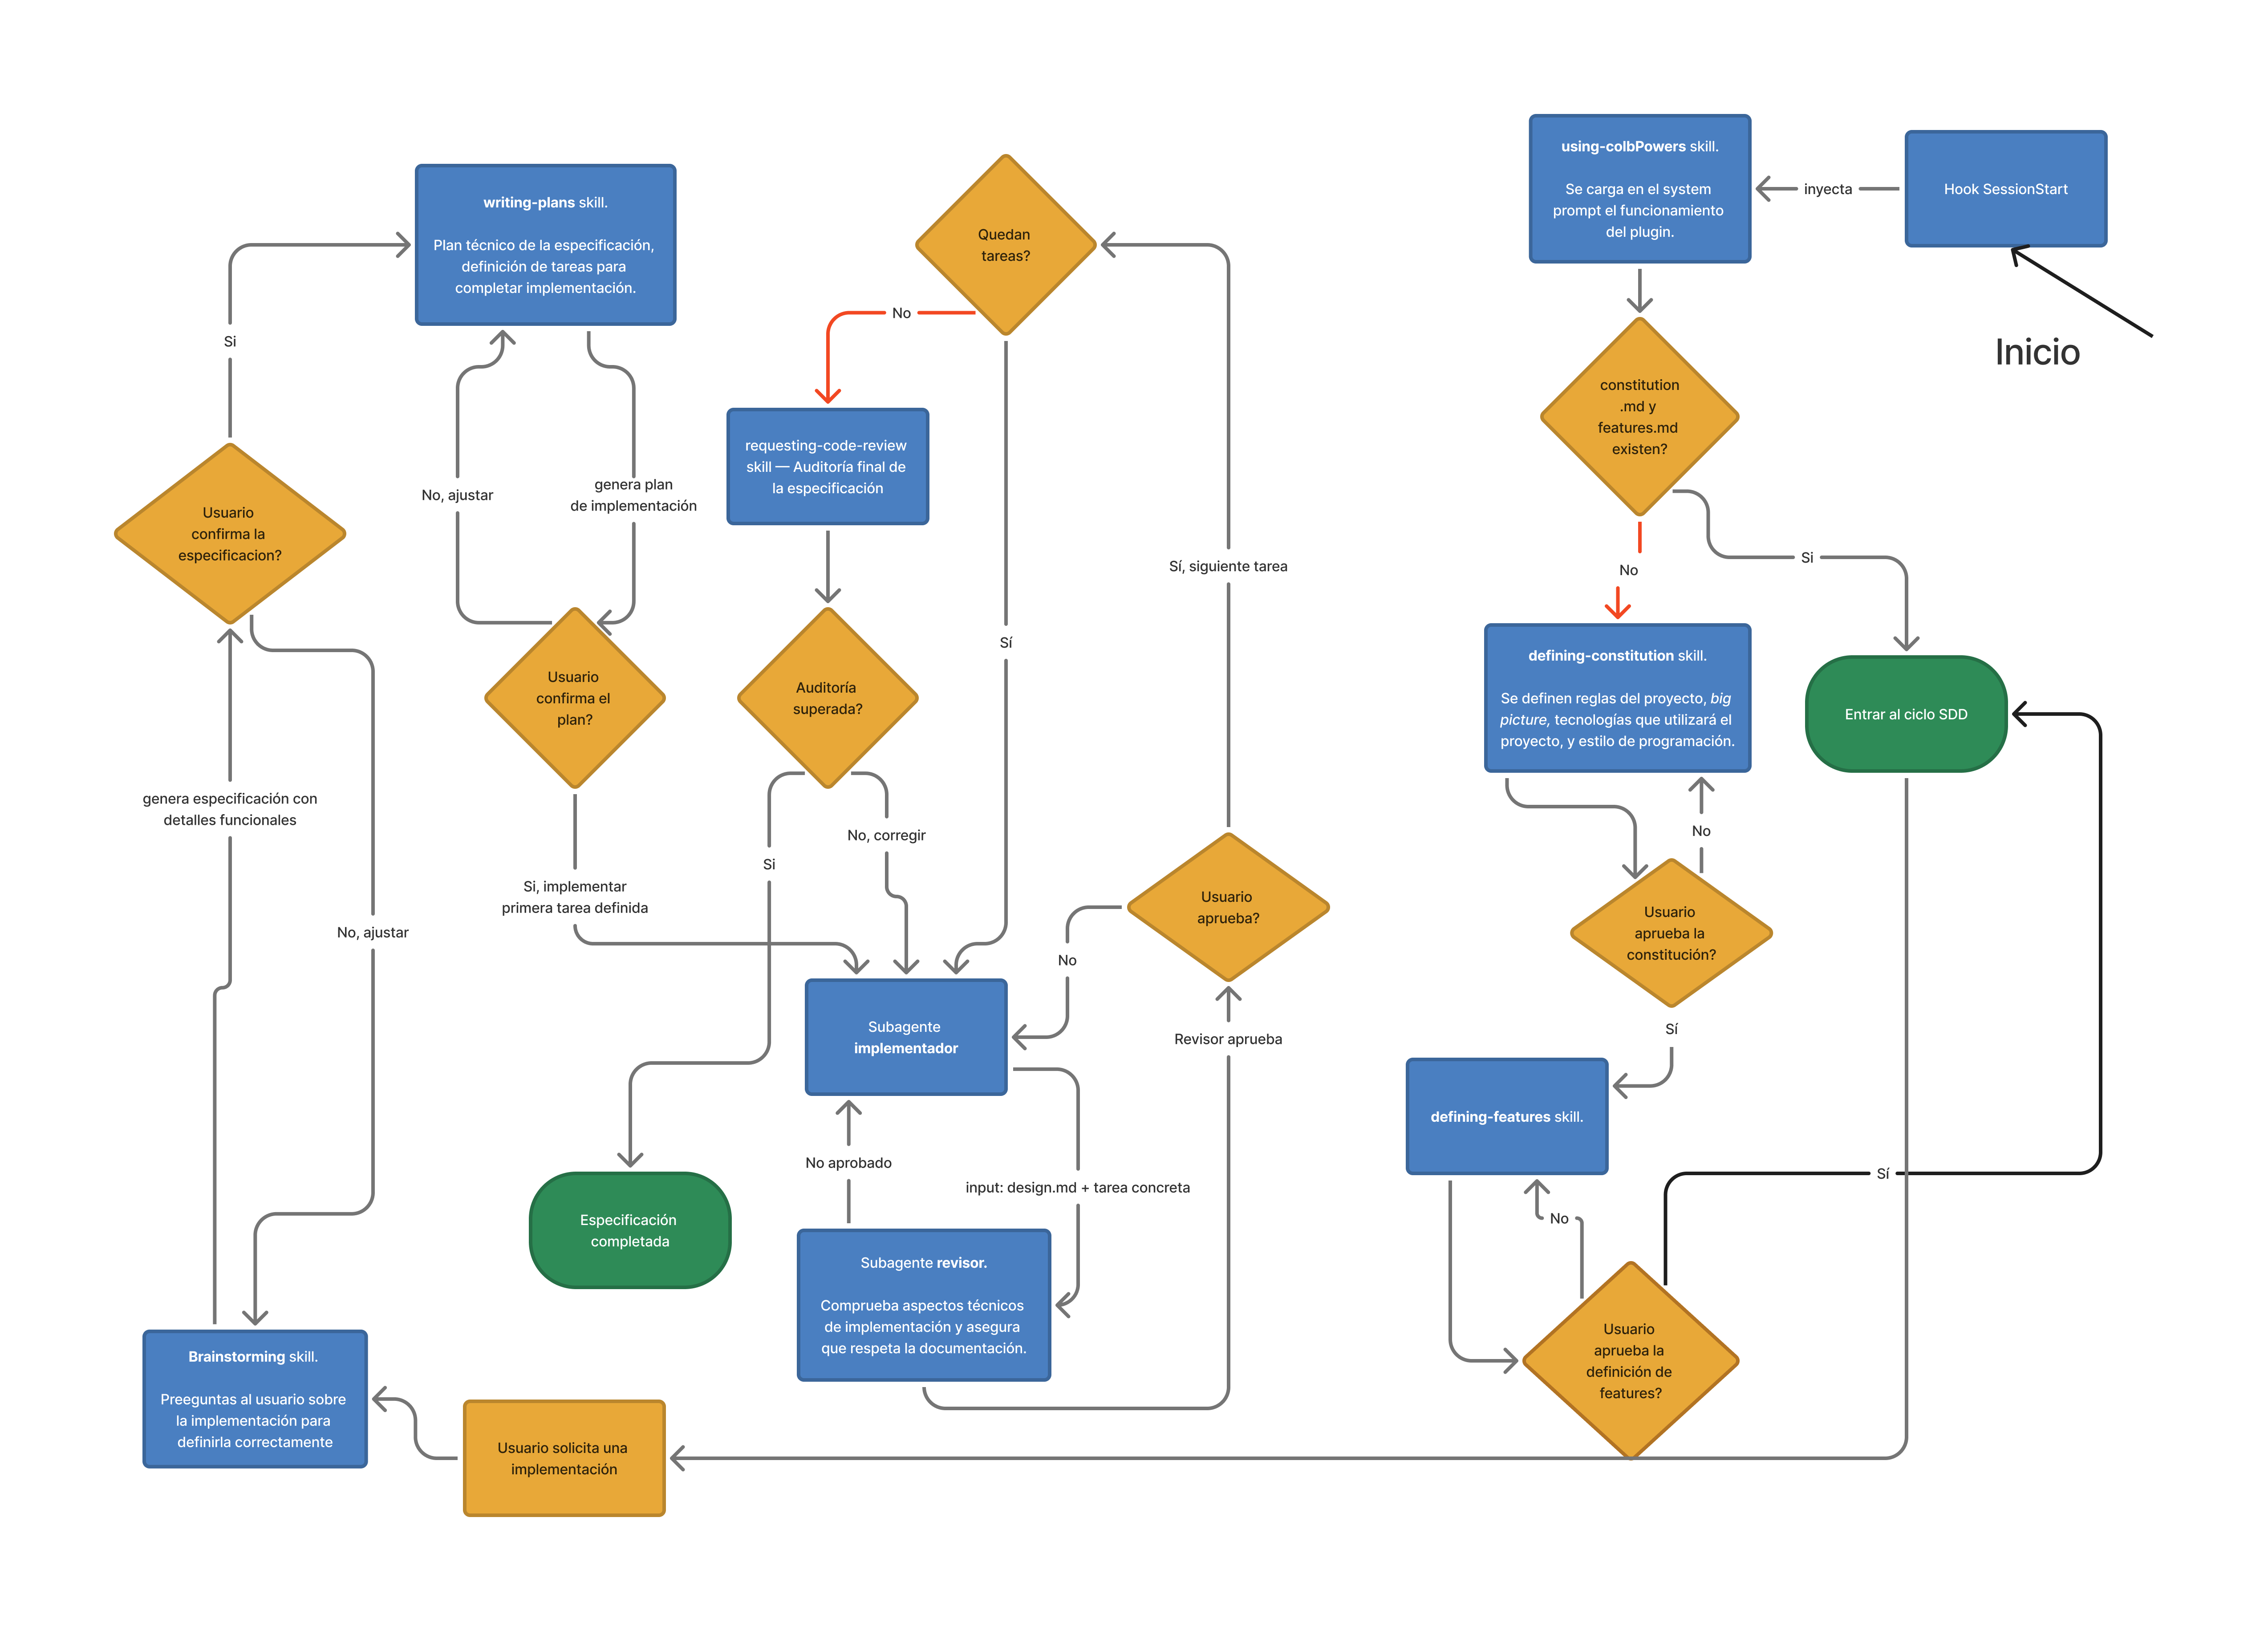
\includegraphics[width=1\textwidth]{imagenes/JustColbPowers.png}
    \caption{Diagrama de flujo de colbPowers. Generación propia.}
    \label{fig:skill_definition}
\end{figure}

\begin{enumerate}
    \item \textbf{Verificación del estado del proyecto:} al iniciar la sesión, el agente lee \texttt{.specs/memory/} y comprueba si existen la constitución y el roadmap de features. Si alguno de los dos está ausente, el agente inicia de forma proactiva una conversación guiada con el usuario para definirlos, formulando preguntas sobre la visión del proyecto, el stack tecnológico, los estándares de código y las funcionalidades previstas. Este paso se ejecuta una única vez por proyecto.
    \item \textbf{Definición interactiva de la especificación:} una vez que los documentos base existen, el agente lleva al usuario por un proceso de preguntas estructuradas para definir con precisión la nueva implementación. Se determina qué debe hacer, a cuál de las features del roadmap pertenece, cuáles son los comportamientos esperados, qué restricciones técnicas aplican y qué criterios de aceptación debe cumplir. El objetivo es eliminar toda ambigüedad antes de escribir una sola línea de código.
    \item \textbf{Generación de la especificación:} cuando el usuario confirma que la definición es correcta, el agente redacta el documento de especificación (design.md) y lo guarda en \texttt{docs/specs/}. Este documento es la fuente de verdad de la implementación y será consultado en cada paso posterior.
    \item \textbf{Generación del plan de implementación:} a partir de la especificación, el agente elabora un plan de tareas (plan.md) en \texttt{docs/plans/} que desglosa la implementación en pasos concretos y ordenados, cada uno con su criterio de aceptación explícito.
    \item \textbf{Ejecución iterativa con implementador y revisor:} el agente utiliza la herramienta de lista de tareas (\texttt{TodoWrite}) integrada en los asistentes CLI para ejecutar el plan de forma iterativa. Para cada tarea, actúa un subagente implementador que escribe el código, y a continuación un subagente revisor que verifica que el código se ajusta a la especificación, sigue el plan y pasa los tests definidos. Cuando estén disponibles, el revisor utilizará además las métricas de calidad de código para evaluar la calidad de la implementación.
\end{enumerate}

\medskip
\noindent\textit{Apunte sobre \texttt{TodoWrite}:} Esta herramienta mantiene el plan de implementación como una lista de tareas con estados explícitos (\textit{pendiente}, \textit{en progreso}, \textit{completada}), visible en todo momento en la interfaz del asistente. Esta visibilidad actúa como ancla de atención: al inicio de cada iteración, el agente consulta la lista para saber exactamente qué tarea tiene en curso y cuál es la siguiente, lo que reduce significativamente la tendencia de los LLMs a desviarse del plan o a saltarse pasos. Cabe mencionar que el runtime no bloquea al agente si este no respeta el orden establecido; la efectividad de \texttt{TodoWrite} como mecanismo de seguimiento proviene de la combinación de la visibilidad explícita del estado y de las instrucciones del sistema que describen su protocolo de uso.

\subsubsection{La plantilla de repositorio}
\label{sec:plantilla_repositorio}
La plantilla de repositorio que colbPowers espera encontrar está diseñada para mantenerse ligera y no imponer burocracia innecesaria. Los únicos documentos imprescindibles son constitution.md y features.md, que el propio agente puede generar desde cero en la primera sesión si no existen. El resto de la estructura (\texttt{docs/specs/}, \texttt{docs/plans/}) se va poblando de forma orgánica a medida que el equipo desarrolla features, convirtiéndose en un registro vivo y trazable de todas las decisiones de diseño del proyecto.

Esta aproximación resuelve uno de los problemas identificados en el análisis del estado del arte: a diferencia de herramientas como Spec Kit, que exigen documentación exhaustiva incluso para cambios pequeños, colbPowers adapta el nivel de formalismo a la magnitud de la tarea. Una corrección menor puede implementarse directamente con el agente; una nueva feature importante pasará por el ciclo completo de especificación, planificación y revisión. El agente decide el nivel de rigor apropiado en cada caso, basándose en el contexto del proyecto y la magnitud del cambio solicitado.

\newpage

\section{Experimentos y evaluación}
\label{sec:evaluacion_resultados}
Con el objetivo de evaluar empíricamente el impacto de las herramientas desarrolladas, se ha ejecutado un experimento controlado que compara dos condiciones ---\textbf{baseline} (herramientas nativas sin plugins) frente a \textbf{colbPowers} (colbPowers~+~code-review-graph)--- sobre dos casos de uso distintos, con dos asistentes de programación y tres repeticiones por condición (n=3) a temperatura~0.

\subsection{Diseño experimental}
\label{sec:diseno_experimental}
Las dos condiciones experimentales son:

\begin{table}[H]
\centering
\begin{tabular}{p{2.4cm} p{4.0cm} p{6.8cm}}
\toprule
\textbf{Condición} & \textbf{Herramientas activas} & \textbf{Descripción} \\
\midrule
\textbf{\texttt{baseline}} & Herramientas nativas CLI & Solo Read, Write, Edit, Bash, Grep. Sin plugins ni servidores MCP adicionales. Actúa como línea base. \\
\textbf{\texttt{colbPowers}} & Nativas + colbPowers + code-review-graph & El agente sigue el flujo SDD de colbPowers con acceso al servidor MCP de code-review-graph. La tarea sigue el ciclo: constitution $\rightarrow$ features $\rightarrow$ spec $\rightarrow$ plan $\rightarrow$ execute $\rightarrow$ review. \\
\bottomrule
\end{tabular}
\caption{Condiciones experimentales. Elaboración propia.}
\label{tab:condiciones_experimentales}
\end{table}

Cada condición se ha ejecutado con dos asistentes: \textbf{OpenCode con DeepSeek V4-Flash}\cite{deepseek_v4_flash} y \textbf{ClaudeCode con Haiku~4.5}\cite{claude_haiku_45}. Las métricas recogidas son: tokens totales consumidos (incluyendo caché), número de tool calls del orquestador, y número de llamadas a herramientas de code-review-graph. En ambos casos se recogen adicionalmente métricas de calidad del código generado (complejidad ciclomática e índice de mantenibilidad) mediante análisis estático: \textbf{radon} \cite{Lacchia_radon} para el Caso~2 (Python) y \textbf{DCM --- Dart Code Metrics} \cite{dart_code_metrics} para el Caso~1 (Flutter/Dart).

\paragraph{Limitaciones del diseño experimental.} Deben señalarse dos limitaciones estructurales. En primer lugar, el tamaño muestral de $n=3$ repeticiones por condición limita la potencia estadística de los resultados e impide verificar los supuestos de normalidad del test $t$ de Welch; los resultados deben interpretarse como evidencia sugerente. En segundo lugar, tanto el diseño de la intervención (colbPowers) como la ejecución y evaluación de los experimentos son obra del mismo autor, en el contexto de la empresa para la que se desarrolla el sistema (Colb.AI). Esta ausencia de evaluación ciega o independiente es una limitación metodológica reconocida, y los resultados deben interpretarse teniendo en cuenta este sesgo potencial.

\paragraph{Metodología:} Para reducir al máximo los sesgos de
confirmación y manipulación involuntaria por parte del experimentador,
se aplica un protocolo de intervención mínima con las siguientes
reglas, ordenadas por prioridad:

\begin{itemize}
    \item \textbf{(P1) Seguridad ante todo:} El experimentador puede
    interrumpir al agente en cualquier momento si detecta que está
    a punto de ejecutar una acción destructiva o peligrosa
    (eliminación de archivos, sobrescritura de datos críticos, etc.).

    \item \textbf{(P2) Solo responder lo que el agente solicite:}
    El experimentador únicamente responde preguntas directas del
    agente o acepta/deniega las solicitudes de permiso que este
    realice explícitamente. No se ofrece información ni correcciones
    de forma proactiva.

    \item \textbf{(P3) Feedback sobre pruebas manuales:} Si el
    agente solicita validación o el experimentador detecta un fallo
    durante las pruebas manuales de la implementación, puede
    comunicar el resultado observado (por ejemplo, que la
    funcionalidad no se comporta como se espera), sin indicar la
    causa ni cómo corregirlo.

    \item \textbf{(P4) Pistas como último recurso:} Solo en caso
    de bloqueo prolongado sin progreso, el experimentador puede
    proporcionar una pista mínima que desbloquee al agente, dejando
    constancia de la intervención en el registro del experimento.
\end{itemize}

\subsection{Caso 1: Aplicación Flutter}
\label{sec:caso1_confortmental}
El primer experimento se llevó a cabo sobre un repositorio real de Colb.AI. Con tal de respetar las políticas de confidencialidad, la descripción del proyecto es lo suficientemente detallada como para entender el contexto, omitiendo ciertos detalles para anonimizarlo.

El proyecto consiste en una aplicación de escritorio desarrollada con el SDK \textit{Flutter}. La tarea asignada al asistente fue la \textbf{eliminación de tres funcionalidades} de la aplicación. Estas funcionalidades eran de naturaleza técnica compleja: una de ellas coordinaba un modelo de IA mediante \textit{LangGraph}, y otras requerían interacción con una base de datos. Su eliminación implicaba identificar y desacoplar código repartido a lo largo de múltiples archivos del repositorio, sin comprometer el resto de la funcionalidad existente.

La hipótesis de partida era que colbPowers obtendría mejores resultados que el baseline en esta tarea por dos razones complementarias. En primer lugar, el servidor MCP \textit{code-review-graph} permitiría al agente explorar el grafo de dependencias del repositorio para identificar con precisión qué entidades de código dependían de las funcionalidades a eliminar, reduciendo el riesgo de dejar referencias huérfanas o eliminar código del que otras partes dependen. En segundo lugar, el flujo de planificación previa de colbPowers ---especificación del alcance de la eliminación y plan de tareas antes de modificar código--- debería producir una intervención más ordenada y con menor complejidad residual que una eliminación directa.

\begin{table}[H]
\centering
\resizebox{\textwidth}{!}{%
\begin{tabular}{l l r r r r r r r r}
\toprule
\textbf{Condición} & \textbf{Ejecución} & \textbf{Total (M)} & \textbf{Input (M)} & \textbf{Output (M)} & \textbf{Caché (M)} & \textbf{Tool calls} & \textbf{CRG} & \textbf{Comp. cic.} & \textbf{Mant. Index} \\
\midrule
\textbf{baseline} & Ejec.~1 & 3,67 & 1,15 & 0,02 & 2,49 & 74 & 0 & 2,67 & 64,85 \\
 & Ejec.~2 & 2,76 & 0,89 & 0,02 & 1,85 & 68 & 0 & 2,84 & 68,66 \\
 & Ejec.~3 & 3,37 & 0,91 & 0,02 & 2,43 & 66 & 0 & 2,50 & 69,27 \\
 & \textbf{Media} & \textbf{3,26} & \textbf{0,98} & \textbf{0,02} & \textbf{2,26} & \textbf{69} & \textbf{0} & \textbf{2,67} & \textbf{67,59} \\
\midrule
\textbf{colbPowers} & Ejec.~1 & 10,64 & 5,40 & 0,07 & 5,15 & 108 & 0 & 3,05 & 69,55 \\
 & Ejec.~2 & 10,55 & 4,18 & 0,07 & 6,27 & 71 & 2 & 3,53 & 65,11 \\
 & Ejec.~3 & 6,95 & 2,61 & 0,05 & 4,27 & 98 & 0 & 3,53 & 65,11 \\
 & \textbf{Media} & \textbf{9,38} & \textbf{4,07} & \textbf{0,06} & \textbf{5,23} & \textbf{92} & \textbf{0,7} & \textbf{3,37} & \textbf{66,59} \\
\bottomrule
\end{tabular}
}
\caption{Caso 1 --- OpenCode con DeepSeek V4-Flash. Caché = tokens leídos de caché. Métricas de calidad calculadas con DCM.}
\label{tab:caso1_opencode}
\end{table}

\begin{table}[H]
\centering
\resizebox{\textwidth}{!}{%
\begin{tabular}{l l r r r r r r r r}
\toprule
\textbf{Condición} & \textbf{Ejecución} & \textbf{Total (M)} & \textbf{Input (M)} & \textbf{Output (M)} & \textbf{Caché (M)} & \textbf{Tool calls} & \textbf{CRG} & \textbf{Comp. cic.} & \textbf{Mant. Index} \\
\midrule
\textbf{baseline} & Ejec.~1 & 6,64 & 0,01 & 0,04 & 6,50 & 76 & 0 & 2,76 & 63,63 \\
 & Ejec.~2 & 2,24 & 0,01 & 0,03 & 2,15 & 44 & 0 & 3,19 & 70,51 \\
 & Ejec.~3 & 2,33 & 0,00 & 0,03 & 2,25 & 38 & 0 & 2,98 & 64,02 \\
 & \textbf{Media} & \textbf{3,74} & \textbf{0,00} & \textbf{0,03} & \textbf{3,63} & \textbf{53} & \textbf{0} & \textbf{2,98} & \textbf{66,05} \\
\midrule
\textbf{colbPowers} & Ejec.~1 & 12,23 & 0,00 & 0,11 & 11,66 & 56 & 0 & 2,97 & 67,03 \\
 & Ejec.~2 & 14,91 & 0,00 & 0,10 & 14,28 & 56 & 0 & 3,53 & 69,03 \\
 & Ejec.~3 & 15,85 & 0,00 & 0,11 & 15,15 & 76 & 3 & 3,94 & 63,51 \\
 & \textbf{Media} & \textbf{14,33} & \textbf{0,00} & \textbf{0,11} & \textbf{13,70} & \textbf{63} & \textbf{1,0} & \textbf{3,48} & \textbf{66,52} \\
\bottomrule
\end{tabular}
}
\caption{Caso 1 --- ClaudeCode con Haiku~4.5. Caché = tokens leídos de caché. Métricas de calidad calculadas con DCM.}
\label{tab:caso1_claudecode}
\end{table}

En ambos asistentes el paso de baseline a colbPowers multiplica el consumo de tokens (x2,9 en OpenCode, x3,8 en ClaudeCode), reflejo del overhead del flujo SDD: generación de documentación estructurada y delegación a múltiples subagentes. El número de tool calls crece moderadamente en OpenCode (69 → 92) y se mantiene similar en ClaudeCode (53 → 63). Las llamadas a code-review-graph son esporádicas: únicamente la Ejecución~2 de OpenCode colbPowers registró 2 llamadas y la Ejecución~3 de ClaudeCode colbPowers registró 3, lo que sugiere que los agentes no incorporaron de forma proactiva el grafo de dependencias para una tarea de tipo exploratorio-visual.

Sin embargo, este sobrecoste de tokens no debe interpretarse en aislamiento. colbPowers genera como subproducto documentación estructurada (constitución del proyecto, especificación de cambios, plan de implementación) que persiste en el repositorio y facilita la incorporación de nuevos desarrolladores. Además, el diseño de colbPowers ---con su énfasis en especificación previa y revisión sistemática--- propicia un ambiente donde los tests forman parte natural del flujo, en lugar de ser un trabajo adicional. En un proyecto de desarrollo profesional con horizonte de vida largo, estos beneficios transcienden el consumo inmediato de tokens.

El desglose de tokens revela una diferencia estructural entre los dos asistentes. En OpenCode, los tokens de entrada no cacheados son significativos (media 0,98~M en baseline, 4,07~M en colbPowers), lo que refleja que cada subagente inicia un contexto propio sin aprovechar caché de sesiones anteriores. En ClaudeCode, en cambio, los tokens de entrada son prácticamente nulos (aprox.\ 0,00~M) y casi la totalidad del consumo corresponde a tokens de caché (3,63~M en baseline, 13,70~M en colbPowers): la API de Anthropic almacena el prefijo del prompt y las peticiones sucesivas leen el contexto desde caché, lo que reduce el coste real pero infla el contador total. Esta asimetría hace que la comparación directa de tokens totales entre OpenCode y ClaudeCode no sea completamente homogénea. 

Las métricas de calidad de código del Caso~1, calculadas con DCM sobre el código modificado, no confirman la hipótesis de partida. En OpenCode, colbPowers produce código de \emph{mayor} complejidad ciclomática (3,37 frente a 2,67 del baseline, $+$26\%) y un índice de mantenibilidad ligeramente inferior (66,59 frente a 67,59, $-$1\%). En ClaudeCode el incremento de complejidad es similar (3,48 frente a 2,98, $+$17\%), mientras que el índice de mantenibilidad se mantiene prácticamente sin cambios (66,52 frente a 66,05).

La explicación más probable reside en que \textit{code-review-graph} apenas fue invocado durante las sesiones: las llamadas registradas fueron en su mayoría cero y en ningún caso más de tres (véase columna CRG en las tablas anteriores), lo que indica que los agentes no aprovecharon el grafo de dependencias para planificar la eliminación. Sin acceso efectivo al contexto de dependencias, el flujo estructurado de colbPowers ---especificación, planificación y revisión--- generó overhead procedimental sin la ventaja de información que habría justificado ese overhead. El resultado neto fue una intervención más fragmentada que la del baseline, con código de limpieza adicional y mayor ramificación residual. En contraste, el agente baseline realizó eliminaciones más directas, produciendo un código resultante estructuralmente más simple aunque sin la documentación ni la trazabilidad del flujo SDD.

Este hallazgo tiene una implicación práctica concreta: el beneficio de colbPowers en tareas de refactorización sobre código existente está condicionado a que el agente utilice efectivamente las herramientas de exploración del repositorio. Cuando \textit{code-review-graph} no es invocado, el flujo SDD puede perjudicar las métricas estáticas respecto al baseline. La Figura~\ref{fig:ttest_cpbl_oc_cm} y la Figura~\ref{fig:ttest_cpbl_cc_cm} muestran los paneles de métricas para el Caso~1.

\subsection{Caso 2: Visualizador de clasificadores en Python}
\label{sec:caso2_simulacion3d}
El segundo caso aplica el experimento sobre una tarea de nueva implementación desde cero: el desarrollo en Python de un visualizador interactivo que muestra, iteración a iteración, cómo dos clasificadores ---\textit{K-Nearest Neighbors} (KNN) y \textit{Logistic Regression}--- aprenden a separar un conjunto de clases en un espacio bidimensional. A diferencia del caso anterior (modificación de una base de código existente), este caso evalúa el comportamiento de las herramientas en la creación de funcionalidad nueva.

Este caso es especialmente relevante para evaluar colbPowers, ya que puede ejecutar el ciclo completo de la metodología SDD: primero se generan de forma interactiva con el usuario los documentos de constitución y \textit{features} del proyecto, y a continuación se genera la especificación técnica de la funcionalidad a implementar. En todo momento el proceso sigue el principio de \textit{Human-in-the-Loop}: el usuario participa en cada etapa y puede controlar el flujo.

\begin{table}[H]
\centering
\resizebox{\textwidth}{!}{%
\begin{tabular}{l l r r r r r}
\toprule
\textbf{Condición} & \textbf{Ejecución} & \textbf{Tokens (M)} & \textbf{Tool calls} & \textbf{CRG} & \textbf{Comp. ciclom.} & \textbf{Mant. Index} \\
\midrule
\textbf{baseline} & Ejec.~1 & 1,59 & 36 & 0 & 4,67 & 44,09 \\
 & Ejec.~2 & 2,52 & 70 & 0 & 4,00 & 39,24 \\
 & Ejec.~3 & 1,53 & 49 & 0 & 4,25 & 41,30 \\
 & \textbf{Media} & \textbf{1,88} & \textbf{52} & \textbf{0} & \textbf{4,31} & \textbf{41,54} \\
\midrule
\textbf{colbPowers} & Ejec.~1 & 6,53 & 80 & 1 & 3,27 & 47,20 \\
 & Ejec.~2 & 10,22 & 86 & 1 & 2,97 & 48,66 \\
 & Ejec.~3 & 8,47 & 89 & 0 & 3,16 & 47,47 \\
 & \textbf{Media} & \textbf{8,41} & \textbf{85} & \textbf{0,7} & \textbf{3,13} & \textbf{47,78} \\
\bottomrule
\end{tabular}
}
\caption{Caso 2 --- OpenCode con DeepSeek V4-Flash.}
\label{tab:caso2_opencode}
\end{table}

\begin{table}[H]
\centering
\resizebox{\textwidth}{!}{%
\begin{tabular}{l l r r r r r}
\toprule
\textbf{Condición} & \textbf{Ejecución} & \textbf{Tokens (M)} & \textbf{Tool calls} & \textbf{CRG} & \textbf{Comp. ciclom.} & \textbf{Mant. Index} \\
\midrule
\textbf{baseline} & Ejec.~1 & 6,12 & 90 & 0 & 2,50 & 49,92 \\
 & Ejec.~2 & 2,75 & 54 & 0 & 3,23 & 62,24 \\
 & Ejec.~3 & 2,37 & 44 & 0 & 2,83 & 58,76 \\
 & \textbf{Media} & \textbf{3,74} & \textbf{63} & \textbf{0} & \textbf{2,85} & \textbf{56,97} \\
\midrule
\textbf{colbPowers} & Ejec.~1 & 7,30 & 46 & 0 & 2,77 & 50,56 \\
 & Ejec.~2 & 6,28 & 44 & 1 & 3,65 & 67,18 \\
 & Ejec.~3 & 10,97 & 55 & 0 & 2,90 & 59,28 \\
 & \textbf{Media} & \textbf{8,19} & \textbf{48} & \textbf{0,3} & \textbf{3,11} & \textbf{59,01} \\
\bottomrule
\end{tabular}
}
\caption{Caso 2 --- ClaudeCode con Haiku~4.5. Elaboración propia.}
\label{tab:caso2_claudecode}
\end{table}

En el segundo caso el sobrecoste de tokens de colbPowers es también significativo (x4,5 para OpenCode, x2,2 para ClaudeCode). En ClaudeCode el orquestador realiza menos tool calls en colbPowers (48) que en baseline (63), lo que confirma que delega la mayor parte del trabajo a subagentes. Las métricas de calidad revelan diferencias notables entre condiciones: en OpenCode, colbPowers genera código de menor complejidad ciclomática (3,13 frente a 4,31, una reducción del 27\%) y mayor índice de mantenibilidad (47,78 frente a 41,54, un incremento del 15\%) que baseline. En ClaudeCode la diferencia es menos pronunciada ---complejidad 3,11 (colbPowers) frente a 2,85 (baseline)---, aunque colbPowers obtiene un índice de mantenibilidad superior (59,01 frente a 56,97, un incremento del 3,6\%). Destaca que ClaudeCode produce código con un índice de mantenibilidad significativamente mayor que OpenCode en ambas condiciones, lo que sugiere una diferencia cualitativa entre los dos asistentes más allá del consumo de recursos.

Estos resultados sugieren que el sobrecoste de tokens de colbPowers compra una mejora real en la estructura del código generado, especialmente en OpenCode. La especificación previa obliga al modelo a reflexionar sobre la arquitectura antes de escribir líneas de código, reduciendo la propensión a soluciones ad-hoc o funciones innecesariamente complejas. Adicionalmente, colbPowers genera por defecto documentación detallada (especificación del comportamiento, plan de implementación, criterios de aceptación) que permanece en el repositorio y facilita el entendimiento futuro del sistema. El flujo estructura también propicia la generación de tests: al exigir criterios de aceptación explícitos en cada tarea, se crea un ambiente natural donde los tests forman parte de la especificación inicial, no un trabajo adicional posterior. Para un proyecto con horizonte de vida extenso, estos beneficios ---código más mantenible, documentación estructurada, propensión a tests--- compensan ampliamente el overhead inicial de tokens.

\subsection{Discusión de los resultados}

\subsubsection{Análisis de consumo}

\paragraph{Baseline vs.\ colbPowers.}
En ambos casos el paso de baseline a colbPowers multiplica el consumo de tokens dentro de cada herramienta: en el Caso~1 el factor es $\times$2,9 para OpenCode y $\times$3,8 para ClaudeCode; en el Caso~2, $\times$4,5 y $\times$2,2 respectivamente. Este sobrecoste refleja el overhead estructural del flujo SDD: generación de documentación (constitution, features, spec, plan), delegación a múltiples subagentes y ejecución de revisiones sistemáticas. La Figura~\ref{fig:tokens_totales} muestra el consumo por experimento, asistente y condición.

\begin{figure}[H]
    \centering
    
\includegraphics[width=\textwidth]{graficos/comparisons/02_tokens_totales.png}
    \caption{Tokens totales por experimento y condición, separados por asistente. La comparación entre columnas de distinto asistente no es directa por diferencias de tokenizador y caché.}
    \label{fig:tokens_totales}
\end{figure}

\begin{figure}[H]
    \centering
    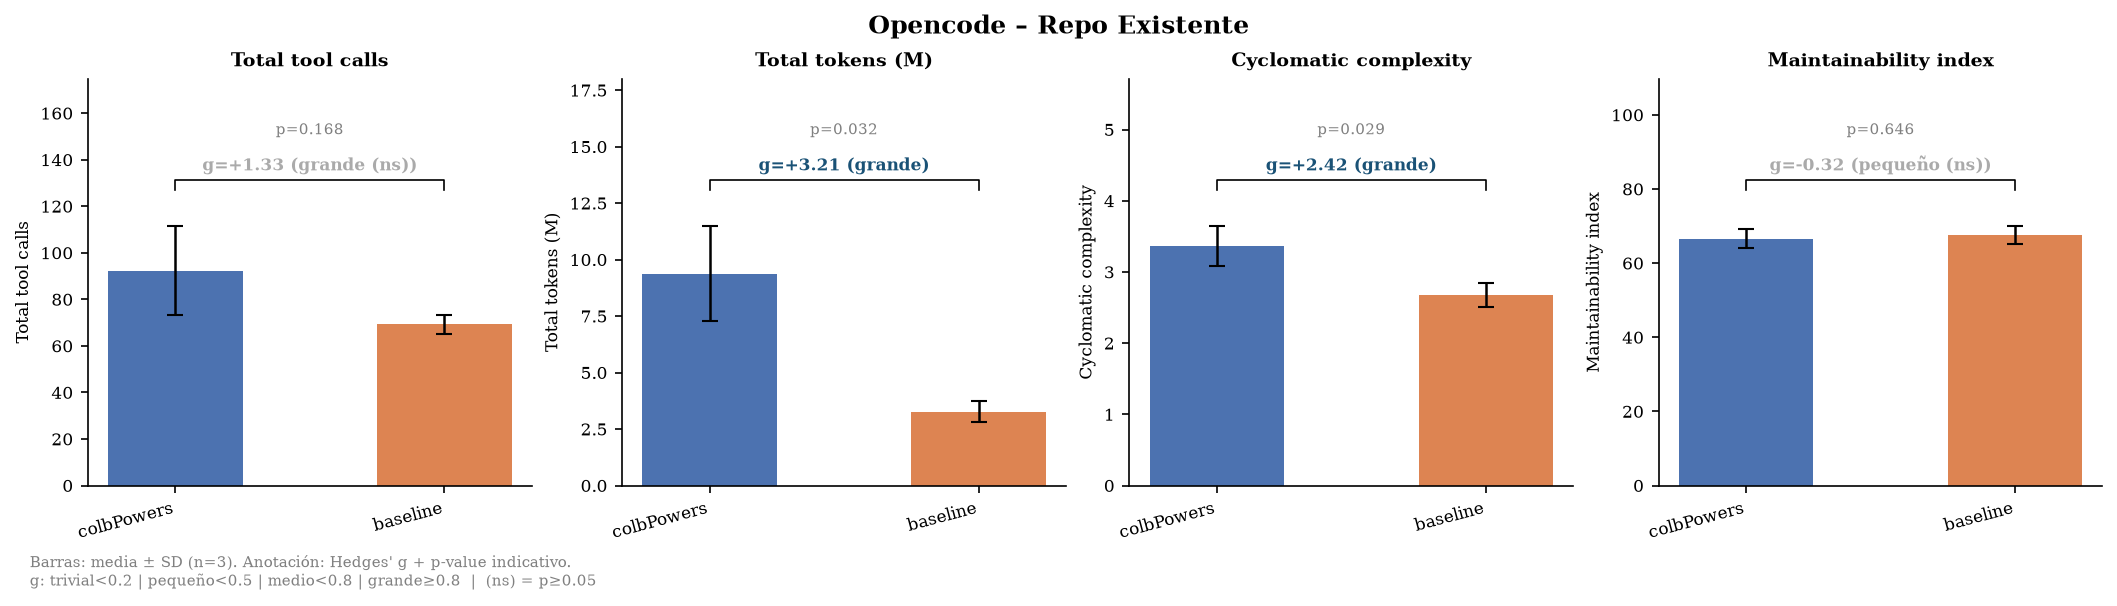
\includegraphics[width=\textwidth]{graficos/ttest_analisis/results_cpbl_bars_Opencode_-_Repo_Existente.png}
    \caption{Test $t$ de Welch — colbPowers vs.\ baseline, OpenCode, Caso~1.}
    \label{fig:ttest_cpbl_oc_cm}
\end{figure}

\begin{figure}[H]
    \centering
    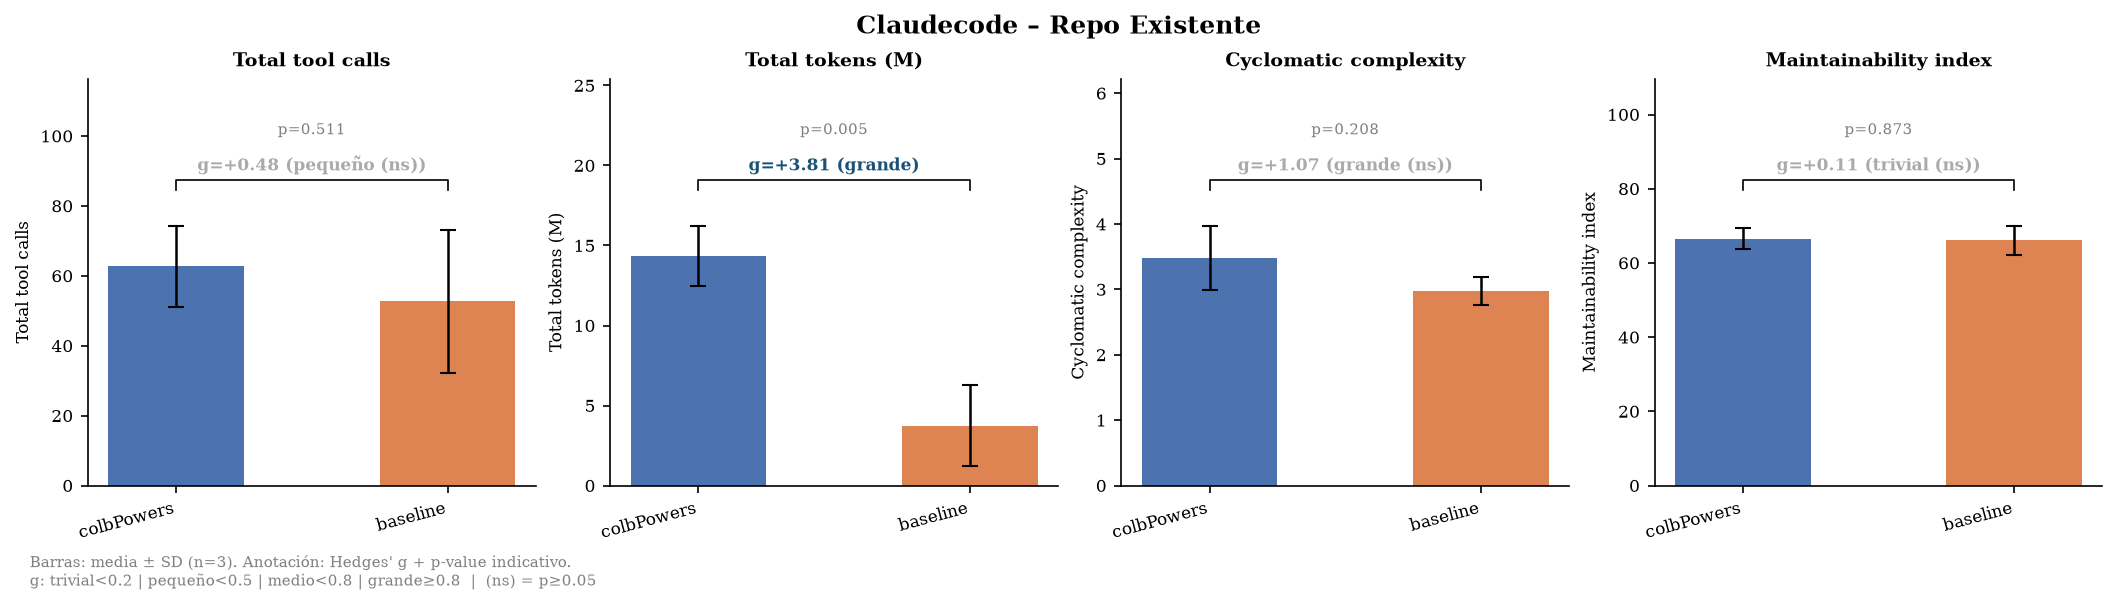
\includegraphics[width=\textwidth]{graficos/ttest_analisis/results_cpbl_bars_Claudecode_-_Repo_Existente.png}
    \caption{Test $t$ de Welch — colbPowers vs.\ baseline, ClaudeCode, Caso~1.}
    \label{fig:ttest_cpbl_cc_cm}
\end{figure}

\textit{Análisis estadístico.} Dado el tamaño muestral reducido ($n=3$ por condición), la $d$ de Cohen se utiliza como métrica principal del tamaño de efecto; los $p$-values del test $t$ de Welch se reportan como referencia indicativa. El sobrecoste de tokens de colbPowers presenta un tamaño de efecto grande en todas las combinaciones donde se dispone de varianza no nula, lo que indica que la diferencia es sustancial con independencia de su significancia estadística formal. El número de tool calls presenta efectos de magnitud menor y más variable entre ejecuciones. Las figuras~\ref{fig:ttest_cpbl_oc_cm} y~\ref{fig:ttest_cpbl_cc_cm} muestran las medias con barras de error (SD) y la $d$ de Cohen para cada comparación en el Caso~1.

\subsubsection{Métricas de calidad}

Las métricas de calidad ---complejidad ciclomática e índice de mantenibilidad--- se calcularon para ambos casos, aunque con herramientas distintas según el lenguaje (DCM para Flutter/Dart en el Caso~1, radon para Python en el Caso~2) y con interpretaciones distintas según el tipo de tarea. En el Caso~1 la discusión cualitativa ya se ha incluido en la sección anterior; el análisis estadístico comparado se presenta a continuación junto con el del Caso~2 para facilitar la comparación entre experimentos.

\paragraph{Baseline vs.\ colbPowers --- Caso~2 (ClassificationVisualization).}
La Figura~\ref{fig:calidad_codigo} muestra las métricas por asistente y condición. En OpenCode, colbPowers produce una reducción de la complejidad ciclomática (de 4,31 a 3,13, un 27\%) y un aumento del índice de mantenibilidad (de 41,54 a 47,78, un 15\%). En ClaudeCode el efecto es menos pronunciado: la complejidad ciclomática aumenta marginalmente (de 2,85 a 3,11) mientras que el índice de mantenibilidad mejora de 56,97 a 59,01 (un 3,6\%).

\begin{figure}[H]
    \centering
    
\includegraphics[width=\textwidth]{graficos/comparisons/01_calidad_codigo.png}
    \caption{Métricas de calidad del código en el Caso~2 por asistente y condición.}
    \label{fig:calidad_codigo}
\end{figure}

La Figura~\ref{fig:delta_calidad} resume estas diferencias como delta (colbPowers $-$ baseline). Las Figuras~\ref{fig:ttest_cpbl_opencode_classvis} y~\ref{fig:ttest_cpbl_claudecode_classvis} presentan los valores absolutos con barras de error (SD) y la $d$ de Cohen.

\begin{figure}[H]
    \centering
    
\includegraphics[width=0.9\textwidth]{graficos/comparisons/08_delta_calidad.png}
    \caption{Efecto de colbPowers sobre la calidad del código (delta = colbPowers $-$ baseline). Verde: mejora; rojo: empeora.}
    \label{fig:delta_calidad}
\end{figure}

\begin{figure}[H]
    \centering
    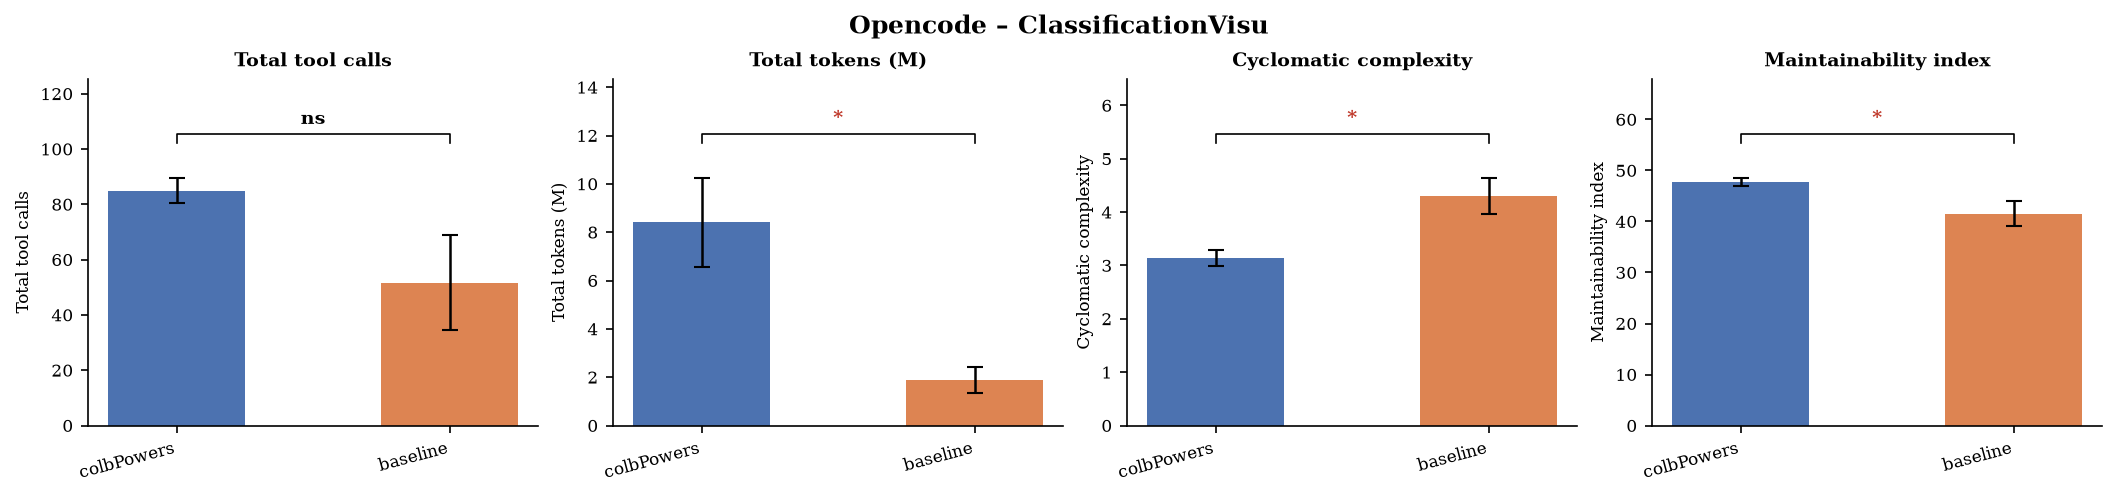
\includegraphics[width=\textwidth]{graficos/ttest_analisis/results_cpbl_bars_Opencode_-_ClassificationVisu.png}
    \caption{colbPowers vs.\ baseline, OpenCode, Caso~2. Barras: media $\pm$ SD. Anotación: $d$ de Cohen y $p$-value indicativo.}
    \label{fig:ttest_cpbl_opencode_classvis}
\end{figure}

\begin{figure}[H]
    \centering
    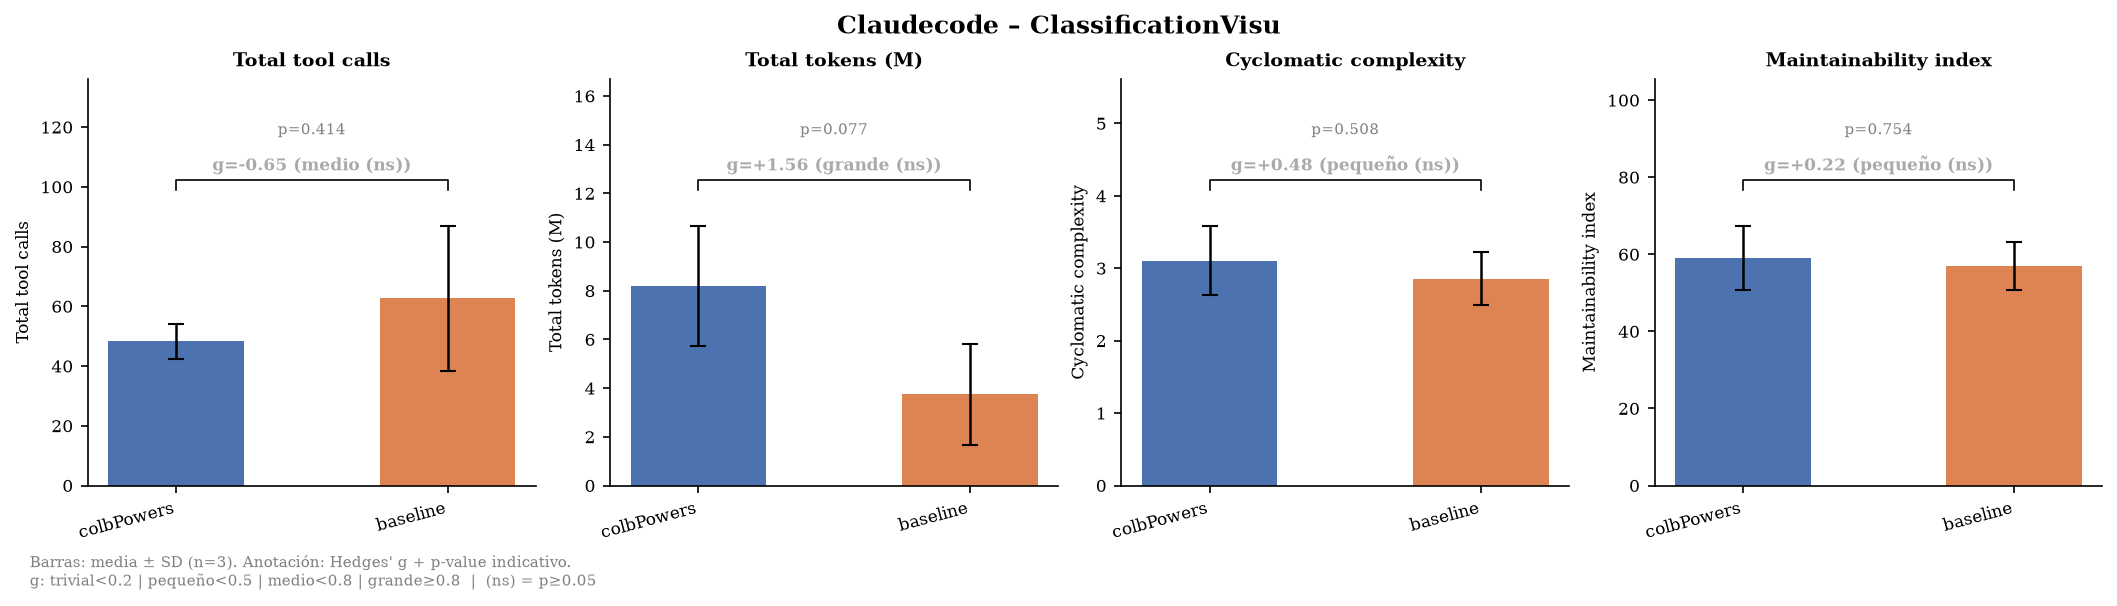
\includegraphics[width=\textwidth]{graficos/ttest_analisis/results_cpbl_bars_Claudecode_-_ClassificationVisu.png}
    \caption{colbPowers vs.\ baseline, ClaudeCode, Caso~2. Barras: media $\pm$ SD. Anotación: $d$ de Cohen y $p$-value indicativo.}
    \label{fig:ttest_cpbl_claudecode_classvis}
\end{figure}

\textit{Análisis estadístico.} En OpenCode, la mejora de calidad con colbPowers presenta un tamaño de efecto grande tanto para la complejidad ciclomática como para el índice de mantenibilidad (véase Figura~\ref{fig:ttest_cpbl_opencode_classvis}), acompañado de $p$-values indicativos ($p=0{,}014$ y $p=0{,}037$ respectivamente). En ClaudeCode, donde la baseline ya produce código de alta calidad, los efectos son consistentes en dirección pero de magnitud considerablemente menor, sin soporte estadístico con $n=3$ (complejidad: $p=0{,}508$; mantenibilidad: $p=0{,}754$).

\paragraph{OpenCode vs.\ ClaudeCode.}
En la condición baseline, ClaudeCode genera código con menor complejidad ciclomática (2,85 frente a 4,31 de OpenCode) y mayor índice de mantenibilidad (56,97 frente a 41,54), lo que sugiere que Haiku~4.5 tiende a producir soluciones más simples y legibles de forma natural. Con colbPowers activo, las diferencias entre asistentes se reducen considerablemente: la complejidad ciclomática converge a valores casi idénticos (3,13 para OpenCode y 3,11 para ClaudeCode), lo que indica que el flujo estructurado de SDD homogeneiza la calidad del código independientemente del asistente.

\begin{figure}[H]
    \centering
    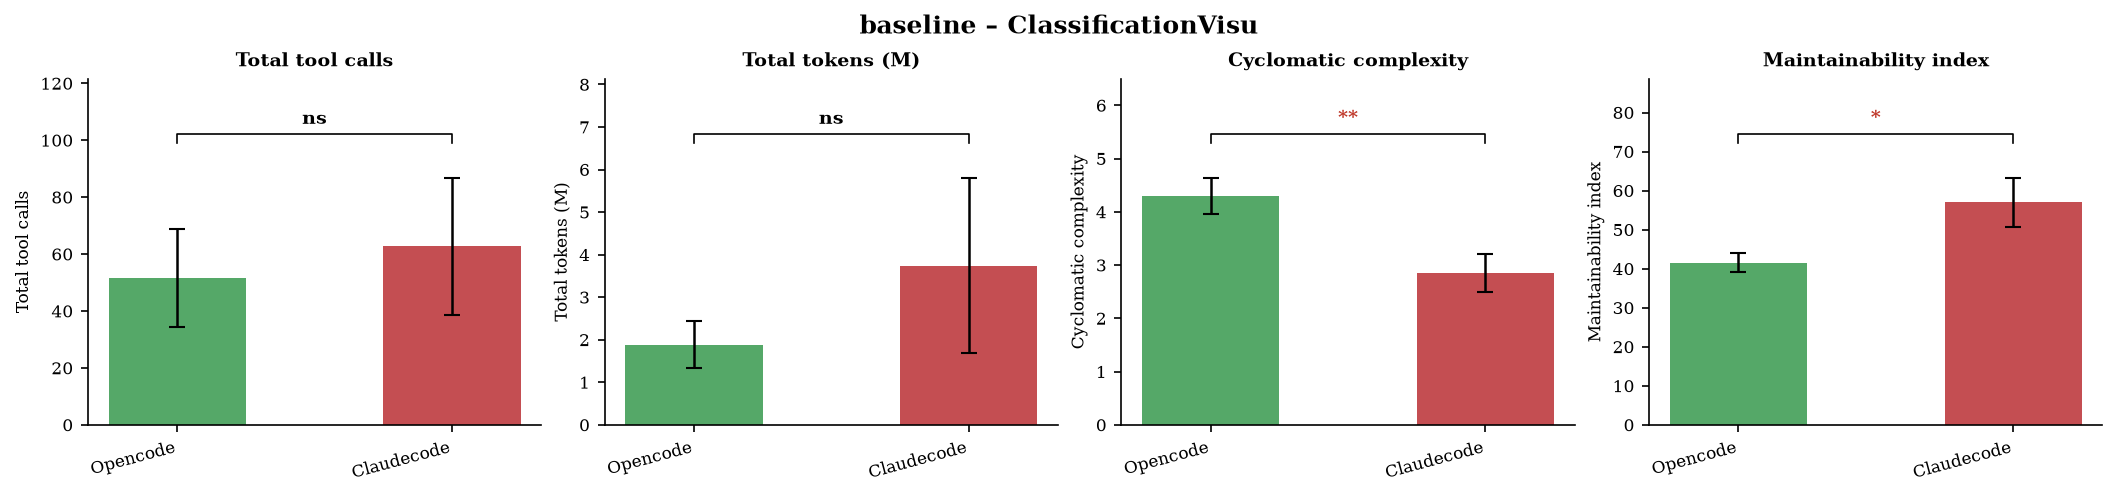
\includegraphics[width=\textwidth]{graficos/ttest_analisis/results_occc_bars_baseline_-_ClassificationVisu.png}
    \caption{OpenCode vs.\ ClaudeCode, baseline, Caso~2. Barras: media $\pm$ SD. Anotación: $d$ de Cohen y $p$-value indicativo.}
    \label{fig:ttest_occc_baseline_classvis}
\end{figure}

\begin{figure}[H]
    \centering
    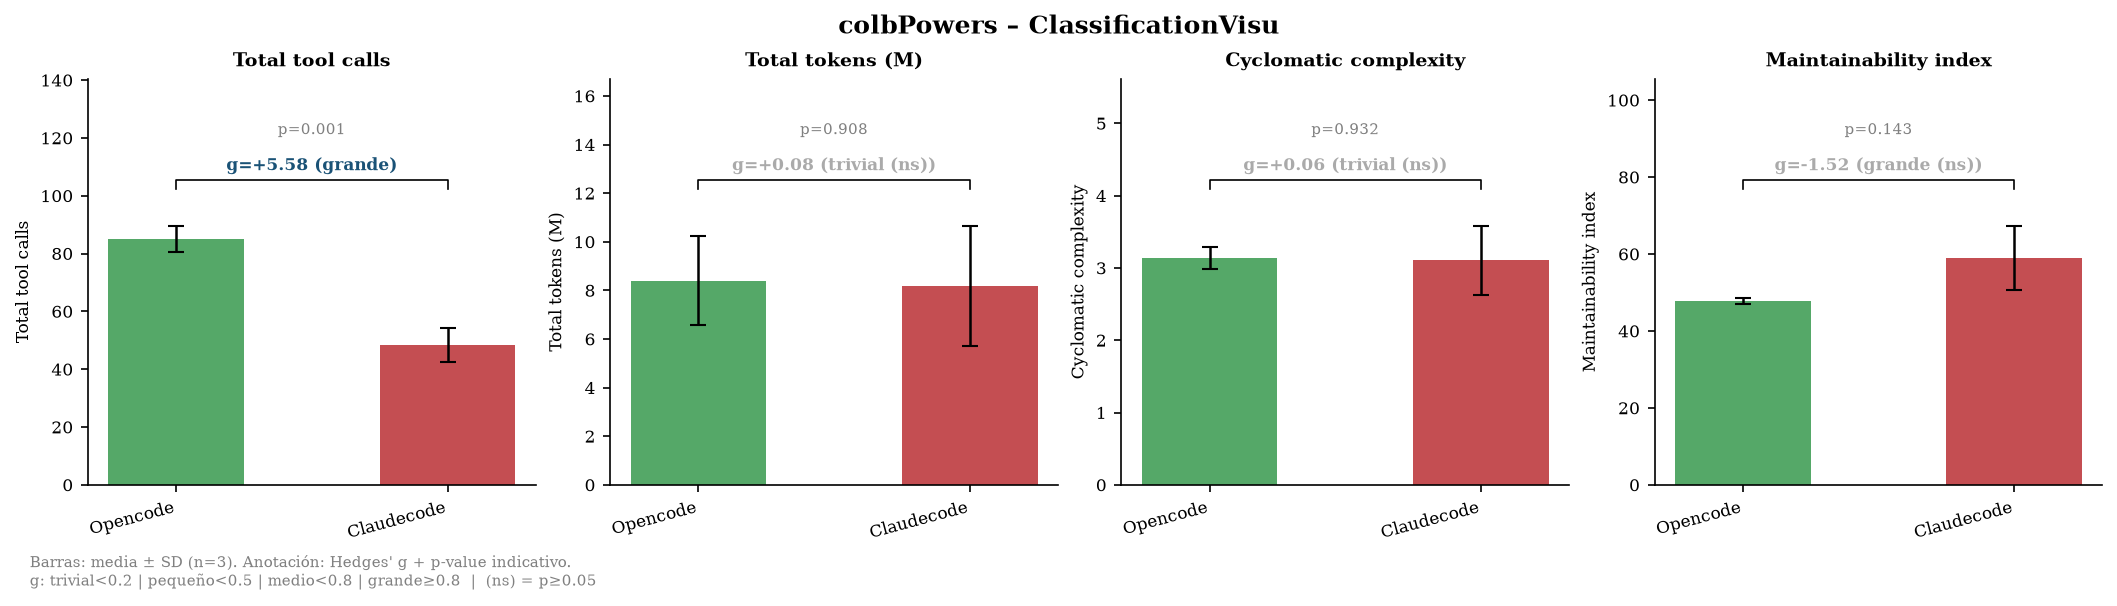
\includegraphics[width=\textwidth]{graficos/ttest_analisis/results_occc_bars_colbPowers_-_ClassificationVisu.png}
    \caption{OpenCode vs.\ ClaudeCode, colbPowers, Caso~2. Barras: media $\pm$ SD. Anotación: $d$ de Cohen y $p$-value indicativo.}
    \label{fig:ttest_occc_colbpowers_classvis}
\end{figure}

\textit{Análisis estadístico.} En la condición baseline, las diferencias de calidad entre asistentes presentan un tamaño de efecto grande (véase Figura~\ref{fig:ttest_occc_baseline_classvis}), con $p$-values indicativos de $p=0{,}007$ para complejidad ciclomática y $p=0{,}039$ para índice de mantenibilidad. Con colbPowers activo, la magnitud de las diferencias se reduce sustancialmente: la $d$ de Cohen cae a valores próximos a cero en ambas métricas, confirmando la convergencia de calidad que propicia el flujo SDD independientemente del asistente.

\paragraph{Baseline vs.\ colbPowers --- Caso~1 (Repo Existente).}
En el Caso~1 el efecto de colbPowers sobre las métricas de calidad es opuesto al del Caso~2: la complejidad ciclomática es mayor en colbPowers que en baseline, tanto en OpenCode (3,37 vs.\ 2,67, $+$26\%) como en ClaudeCode (3,48 vs.\ 2,98, $+$17\%). El índice de mantenibilidad se mantiene prácticamente sin cambios en ClaudeCode (66,52 vs.\ 66,05) y cae marginalmente en OpenCode (66,59 vs.\ 67,59, $-$1\%). Este resultado no confirma la hipótesis de que \textit{code-review-graph} proporcionaría un contexto de dependencias superior: las llamadas al servidor MCP fueron prácticamente nulas en todas las ejecuciones, lo que privó al flujo SDD de la ventaja de exploración que habría justificado su overhead. Los paneles de calidad en las Figuras~\ref{fig:ttest_cpbl_oc_cm} y~\ref{fig:ttest_cpbl_cc_cm} muestran estos valores con barras de error (SD) y la $d$ de Cohen correspondiente.

\paragraph{OpenCode vs.\ ClaudeCode --- Caso~1.}
En el Caso~1, a diferencia del Caso~2, las diferencias de calidad entre asistentes son menos pronunciadas. En la condición baseline, ambos producen complejidad ciclomática similar (OpenCode 2,67, ClaudeCode 2,98) e índice de mantenibilidad comparable (67,59 vs.\ 66,05). Con colbPowers, la brecha es igualmente pequeña (3,37 vs.\ 3,48 en complejidad; 66,59 vs.\ 66,52 en mantenibilidad). Esto sugiere que en tareas de modificación incremental la elección del asistente tiene menor impacto en la calidad estructural del código producido.

\begin{figure}[H]
    \centering
    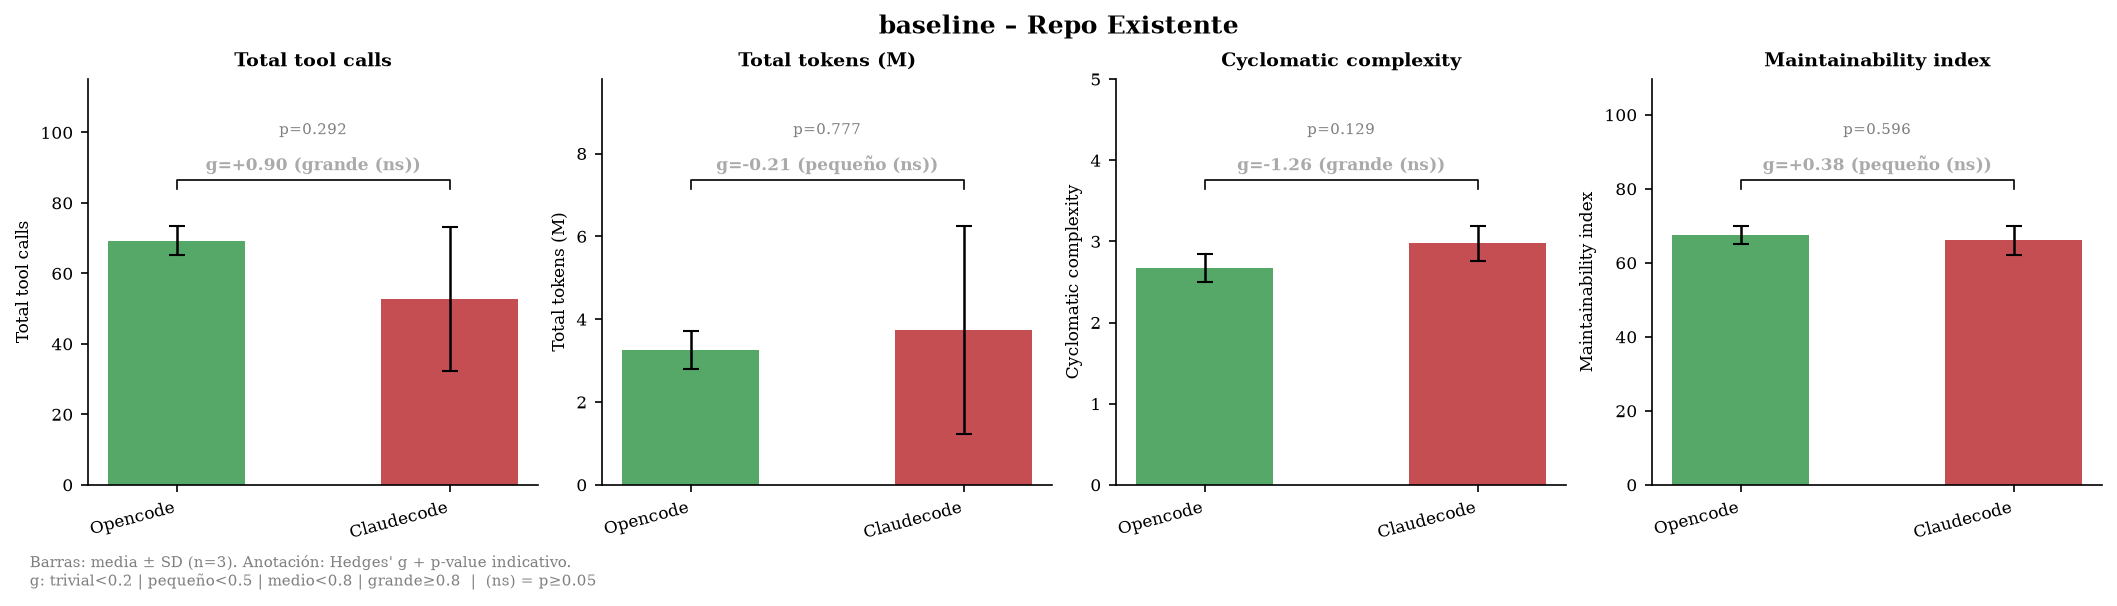
\includegraphics[width=\textwidth]{graficos/ttest_analisis/results_occc_bars_baseline_-_Repo_Existente.png}
    \caption{OpenCode vs.\ ClaudeCode, baseline, Caso~1. Barras: media $\pm$ SD. Anotación: $d$ de Cohen y $p$-value indicativo.}
    \label{fig:ttest_occc_baseline_caso1}
\end{figure}

\begin{figure}[H]
    \centering
    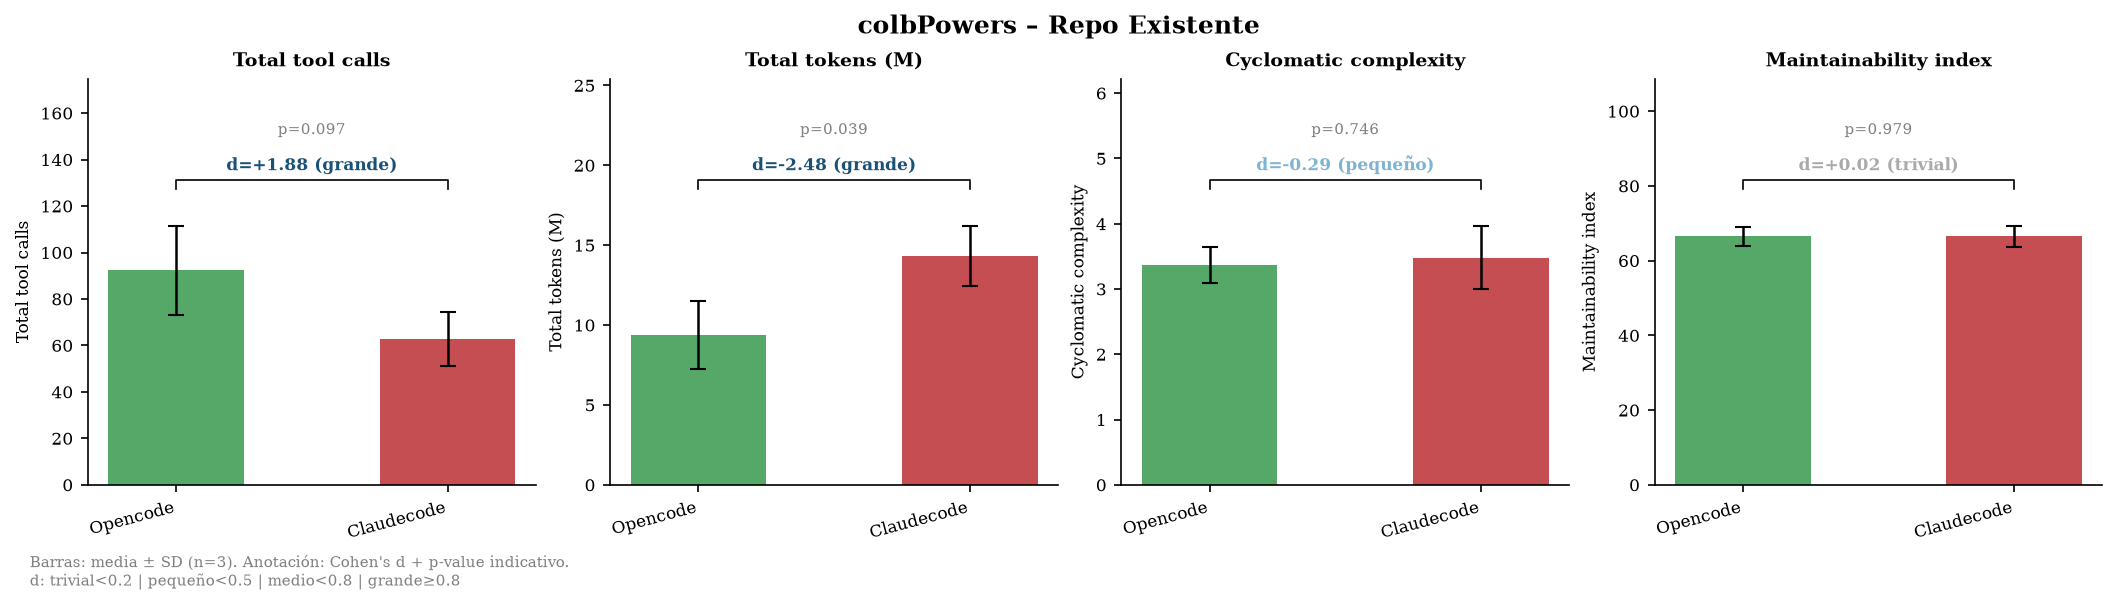
\includegraphics[width=\textwidth]{graficos/ttest_analisis/results_occc_bars_colbPowers_-_Repo_Existente.png}
    \caption{OpenCode vs.\ ClaudeCode, colbPowers, Caso~1. Barras: media $\pm$ SD. Anotación: $d$ de Cohen y $p$-value indicativo.}
    \label{fig:ttest_occc_colbpowers_caso1}
\end{figure}

Las tablas completas del análisis estadístico se recogen en el Anexo~\ref{sec:anexo_ttest}.

\newpage

\section{Integración de conocimientos}
\label{sec:integracion_conocimientos}

\subsection{Competencias técnicas del proyecto}
\label{sec:competencias_tecnicasa}
En esta sección se va a asociar las competencias técnicas asignadas al proyecto y los conocimientos aplicados en el desarrollo de este.
\begin{itemize}
    \item\textbf{CCO1.3: Definir, evaluar y seleccionar plataformas de desarrollo y producción hardware y software para el desarrollo de aplicaciones y servicios informáticos de diversa complejidad. [Un poco]} El proyecto evalúa y selecciona herramientas para cada módulo del sistema: ClaudeCode y OpenCode como asistentes CLI frente a extensiones de IDE o frameworks de bajo nivel, Azure Speech Service frente a Whisper para la transcripción con diarización, y Tavily frente a APIs de búsqueda convencionales para la búsqueda semántica orientada a agentes. Cada decisión está justificada por criterios técnicos y de integración con el ecosistema de Colb.AI.
    \item\textbf{CCO2.1: Demostrar conocimiento de los fundamentos, paradigmas y técnicas de los sistemas inteligentes, y analizar, diseñar y construir sistemas, servicios y aplicaciones informáticas que utilicen estas técnicas. [En profundidad]} Este proyecto diseña e implementa un sistema multi-agente basado en el patrón ReAct (Reasoning + Acting), el paradigma estándar para la construcción de agentes sobre LLMs. Se diseña una arquitectura con orquestador y subagentes aislados, se implementa la gestión del ciclo de vida de sesión mediante hooks, y se aplica ingeniería de prompts como mecanismo de control del comportamiento.
    \item\textbf{CCO2.2: Capacidad para adquirir, obtener, formalizar y representar el conocimiento humano de forma computable para la resolución de problemas mediante un sistema informático. [Bastante]} El módulo de toma de requisitos convierte conversaciones informales con clientes en especificaciones técnicas computables. El pipeline adquiere el conocimiento (grabación y transcripción), extrae el contenido relevante (chunking y filtrado configurable), y lo formaliza en documentos estructurados (constitution.md, features.md, design.md) que los agentes del sistema pueden leer y sobre los que pueden razonar. La diarización de hablantes permite distinguir qué restricciones provienen del cliente y cuáles del equipo técnico.
    \item\textbf{CCO2.5:  Implementar software de búsqueda de información (information retrieval). [En profundidad]} En la toma de requisitos, el pipeline identifica automáticamente las decisiones tecnológicas abiertas y formula queries de búsqueda que se ejecutan sobre Tavily, motor que combina recuperación léxica con re-ranking semántico por similitud de coseno. En el módulo SDD, codereview-graph construye un grafo de dependencias del repositorio mediante Tree-Sitter y lo expone al agente como un servicio de búsqueda semántica sobre entidades del código, con cálculo de blast radius. Las herramientas de IR son de terceros, la contribución del proyecto reside en el diseño del pipeline que las rodea.

\end{itemize}

\subsection{Asignaturas}
\label{sec:asignaturas}
En este apartado se presentan las asignaturas de las cuales se han podido utilizar conocimientos que aplicar al proyecto.

\begin{itemize}
    \item \textbf{Compresión de datos e imágenes (CDI):} Para la implementación propia del módulo de transcripción, se utiliza ffmpeg con técnicas de compresión vistas en CDI, para que el proceso de transcripción tarde menos sin perder demasiada calidad. Principalmente, se aplica un \textit{Downsampling} ---reducción en el muestreo del audio--- y luego se convierte a MP3 mono, formato que aprovecha la compresión con pérdida basada en MDCT (\textit{Modified Discrete Cosine Transform}) y modelado psicoacústico para reducir significativamente el tamaño del archivo.
    \item \textbf{Búsqueda y analisis de información masiva (CAIM):} Del apartado de \textit{Local Sensitive Hashing} de la asignatura, se extrajo la idea de almacenar los audios transcritos con sus respectivos hashes, aunque en la implementación no se utiliza ningún método de \textit{LSH}, se utiliza un hash criptográfico SHA-256 para identificación exacta del contenido. Los apartados de \textit{Web, Information Retrieval} fueron de utilidad para entender y implementar servicios como \textit{Tavily} para la búsqueda web, así como el temario de \textit{Networks} para la formación de el grafo de \textit{code-review-graph}, que facilita a los asistentes de programación la búsqueda y exploración del código.
    \item \textbf{Introducción a la ingeniería del software (IES):} La base proporcionada en esta asignatura sobre requisitos de software, diseño de sistemas y creación de diagramas de flujo, fueron extremadamente útiles tanto para planificar el sistema implementado en este proyecto.
\end{itemize}

\newpage

\section{Conclusiones}
\label{sec:conclusiones}

\subsection{Conclusiones generales}
\label{sec:conclusiones_generales}

Este trabajo ha abordado un problema relevante en el desarrollo de software asistido por inteligencia artificial: la tendencia del paradigma \textit{Code-Driven} a generar código de baja calidad estructural cuando no existe una fase previa de especificación y planificación. La propuesta central del proyecto ---el plugin colbPowers y el flujo \textit{Spec-Driven Development} (SDD)--- ha demostrado ser técnicamente viable y empíricamente evaluable dentro del entorno de trabajo de Colb.AI.

\subsubsection*{Cumplimiento de objetivos}

El sistema cumple los cuatro sub-objetivos funcionales y arquitectónicos establecidos al inicio del proyecto. Se ha conseguido una separación efectiva de responsabilidades mediante subagentes especializados (implementador, revisor de código y revisor de coherencia con especificaciones); se mantiene coherencia arquitectónica entre sesiones gracias a \texttt{constitution.md} y \texttt{features.md} como fuente de verdad compartida; los agentes pueden ejecutar acciones reales y verificables sobre el repositorio; y existe trazabilidad completa entre la especificación y el código entregado a través del historial git. Los módulos de toma de requerimientos y seguimiento del cliente completan la cobertura del ciclo de vida del software, desde la primera reunión con el cliente hasta la entrega y seguimiento iterativo.

\subsubsection*{Resultados experimentales}

La evaluación experimental produce resultados mixtos pero coherentes. Dado el tamaño muestral ($n=3$ por condición), la $d$ de Cohen se utiliza como métrica principal del efecto; los $p$-values del test $t$ de Welch se reportan como referencia indicativa. El hallazgo principal es la mejora con tamaño de efecto grande en las métricas de calidad del código en el Caso~2 (proyecto generado desde cero): colbPowers reduce la complejidad ciclomática un 27\% y mejora el índice de mantenibilidad un 15\% en OpenCode, con $p$-values indicativos de $p=0{,}014$ y $p=0{,}037$ respectivamente. Con ClaudeCode, que de base produce código de mayor calidad, los efectos son consistentes en dirección pero de magnitud considerablemente menor, sin soporte estadístico con $n=3$. En el Caso~1 (eliminación de funcionalidades complejas sobre un repositorio existente), el patrón se invierte: colbPowers produce código de mayor complejidad ciclomática (+17--26\%) sin mejora neta en mantenibilidad. El factor determinante parece ser que los agentes no invocaron \textit{code-review-graph} de forma efectiva, privando al flujo SDD del contexto de dependencias que habría justificado su overhead. Sin ese contexto, la planificación estructurada generó código de limpieza adicional más complejo que las eliminaciones directas del baseline.

Un resultado secundario con implicaciones prácticas directas es la convergencia de calidad entre asistentes: con colbPowers activo, la $d$ de Cohen entre OpenCode y ClaudeCode cae a valores próximos a cero en ambas métricas de calidad. Esto indica que el flujo SDD homogeneiza la calidad del código con independencia del asistente, lo que permite a un equipo combinar herramientas distintas sin comprometer la consistencia del producto.

El coste del sistema es real y cuantificado: colbPowers multiplica el consumo de tokens por un factor de entre 2{,}9× y 4{,}5× respecto al baseline, con tamaños de efecto grandes en todas las combinaciones evaluadas. Este sobrecoste refleja el \textit{overhead} inherente al flujo SDD y debe considerarse una variable de diseño, no un defecto: el sistema intercambia recursos computacionales por mayor calidad estructural del código producido.

\subsubsection*{Limitaciones}

El diseño experimental con $n=3$ repeticiones por condición tiene potencia estadística limitada e impide verificar los supuestos de normalidad requeridos por el test $t$ de Welch. Los resultados deben considerarse evidencia sugerente, no concluyente, y deberán ser confirmados con tamaños muestrales mayores ($n \geq 5$) en trabajos futuros. Adicionalmente, las herramientas de análisis estático empleadas difieren entre casos ---radon para Python y DCM para Flutter/Dart---, lo que implica que las métricas de calidad no son directamente comparables entre experimentos, aunque sí lo son dentro de cada caso entre condiciones. Por último, el mecanismo de garantía del flujo SDD es no determinista: en algunos experimentos el agente orquestador omitió la invocación del subagente revisor, lo que indica que la garantía de proceso es una restricción de comportamiento ---a nivel de prompt--- y no una restricción de ejecución.

\subsubsection*{Valoración global}

La hipótesis principal del proyecto ---que estructurar el desarrollo mediante un flujo SDD mejora la calidad del código generado--- ha recibido soporte empírico preliminar en el contexto evaluado. Los resultados justifican continuar investigando el enfoque, ampliar el tamaño muestral y extender las métricas de evaluación a otros lenguajes y tipos de proyecto. La contribución técnica del TFG ---un plugin funcional, dos módulos de apoyo y un conjunto de datos experimentales cuantificables sobre el efecto del flujo SDD--- proporciona una base concreta para este trabajo futuro.

\subsection{Trabajo futuro}
\label{sec:trabajo_futuro}

A continuación se describen las líneas de mejora y expansión identificadas durante el desarrollo del proyecto, organizadas por componente del sistema.

\subsubsection{Plugin colbPowers y flujo SDD}

\paragraph{Refuerzo determinista del flujo mediante hooks.}
El mecanismo actual para asegurar que el agente orquestador siga el flujo SDD se basa exclusivamente en el prompt de instrucciones, lo que es inherentemente no determinista: en los experimentos se observaron casos en los que el orquestador omitió la llamada al subagente revisor tras implementar código. Una mejora natural sería reemplazar parte de esta responsabilidad por hooks de ciclo de vida que comprueben el estado del flujo en puntos clave y bloqueen el avance si no se han completado los pasos requeridos. Esto transformaría una restricción de comportamiento en una restricción de ejecución, más robusta y reproducible.

\paragraph{Mayor presencia de code-review-graph en los archivos de contexto.}
Los experimentos mostraron que el servidor MCP \textit{code-review-graph} fue prácticamente ignorado por los agentes: las llamadas registradas fueron esporádicas y en su mayoría no iniciadas por el orquestador. Una causa probable es que el orquestador no transmitía a los subagentes información sobre la disponibilidad y el propósito del servidor. Añadir instrucciones explícitas en los archivos de contexto del agente ---indicando cuándo y cómo utilizar el grafo de dependencias--- podría incrementar significativamente su adopción y, con ello, la calidad del análisis de impacto previo a cada cambio.

\paragraph{Experimentos adicionales.}
Los experimentos realizados requieren supervisión manual continua, lo que limitó el tamaño muestral a $n=3$ por condición. Con más recursos, se proponen las siguientes comparaciones:
\begin{itemize}
    \item \textbf{colbPowers con y sin code-review-graph}, para aislar el efecto del servidor MCP de forma independiente al resto del flujo.
    \item \textbf{colbPowers vs a superpowers}, su plugin predecesor, para cuantificar el valor añadido de las extensiones introducidas en este proyecto.
    \item \textbf{Ejecución inline vs a subagent-driven}, para evaluar si el overhead de tokens de la ejecución por subagentes se traduce en mejoras de calidad consistentes respecto a que el orquestador resuelva las tareas directamente.
\end{itemize}
En todos los casos se recomendaría aumentar el número de iteraciones a $n \geq 5$ para poder aplicar tests no paramétricos (que con $n=3$ no pueden alcanzar $p<0{,}05$) y obtener estimaciones más robustas del tamaño de efecto.

\subsubsection{Módulos de transcripción y documentación}

\paragraph{Memoria acumulativa entre reuniones.}
Actualmente, tanto el módulo de toma de requerimientos como el de seguimiento del cliente procesan cada reunión de forma completamente independiente, sin acceso al historial de sesiones anteriores. Esto obliga al equipo a proporcionar manualmente el contexto acumulado en cada nueva ejecución. Una mejora sustancial consistiría en incorporar un almacén persistente ---por ejemplo, una base de datos vectorial--- que indexe los documentos generados en reuniones previas y permita al modelo recuperar contexto relevante mediante búsqueda semántica. Esto haría los documentos generados más coherentes con la evolución del proyecto a lo largo del tiempo.

\paragraph{Base de datos RAG para estimaciones de presupuesto y horas.}
El módulo de toma de requerimientos genera estimaciones de tiempo y coste por funcionalidad basándose únicamente en el razonamiento del modelo, sin datos históricos de referencia. Incorporar una base de datos de recuperación aumentada (\textit{Retrieval-Augmented Generation}) con ejemplos reales de proyectos anteriores ---incluyendo desglose de horas por tipo de tarea y presupuestos asociados--- permitiría al módulo fundamentar sus estimaciones en precedentes concretos, aumentando su fiabilidad y utilidad práctica para la planificación de proyectos.

\paragraph{Integración con herramientas de gestión de proyectos.}
El documento de seguimiento generado actualmente es un artefacto estático en formato Word. Un paso natural sería integrarlo con plataformas de gestión de proyectos como Linear o Jira, de modo que las tareas identificadas en la reunión se conviertan automáticamente en tickets asignados, con descripción, estimación y responsable. Esto cerraría el ciclo entre la reunión con el cliente y el flujo de trabajo del equipo de desarrollo sin intervención manual.

\paragraph{Reducción de la dependencia de Claude Cowork.}
Ambos módulos disponen de una implementación propia de código abierto como alternativa a la skill de Claude Cowork, pero esta alternativa no cubre todos los casos de uso de la plataforma comercial. Consolidar y extender las implementaciones propias reduciría la dependencia de una suscripción externa y facilitaría el despliegue del sistema en entornos con requisitos de privacidad o control de costes estrictos.

\newpage

\section{Cosas en proceso y dudas}
A continuación se listan las cosas que considero que están pendientes en la memoria y voy a implementar en los próximos dias. Están ordenadas según lo que yo consideraría ser la prioridad (más prioritarias primero).
\begin{enumerate}
    \item \textbf{Escribir los abstracts:} He de escrir el abstracts en Catalán, Castellano y Ingles.  (Cubierto, pendiente de revisiones)
    \item \textbf{Debería eliminar el apartado de Integración de conocimiento?} El apartado de integración del conocimiento nos lo pedian para el informe de seguimiento, pero la verdad es que no aporta absolutamente nada en mi opinión... Se podría quitar.
    \item \textbf{Acabar de comentar los experimentos en mayor detalle:} Los experimentos han sido comentados y se han añadido graficas para comparar las difereentes configuraciones, pero se puede expandir bastante este apartado. He hecho un script para hacer un estudio estadístico de los resultados, me falta añadirlo. También tengo un montón de graficos que no he puesto en el apartado pero podrian ir a un posible Anexo. (Medio hecho)
    \item \textbf{Conclusiones y trabajo futuro:} Aún queda escribir este apartado. (Trabajo futuro cubierto)
    \item \textbf{Apartado de "Uso de IA en el proyecto":} Compañeros mios han implementado un apartado que me parecería muy interesante de mencionar. Básicamente consiste en hacer una explicación de que usos se le han dado a la IA generativa para el desarrollo del proyecto, puesto que la he utilizado para hacer brainstorming, asistencia en la programación de modulos del proyecto, y ha ayudado a formular secciones de la memoría. Por supuesto se ha hecho con el máximo cuidado para evitar que haya basura, pero aún así considero que no es mala idea para tener una máxima transparencia hacer un tipo de disclaimer. (Cubiero en el aparado \ref{sec:uso_ia})
    \item \textbf{Apartado de "Sistema completo":} Me gustaría añadir un apartado en el que explique el funcionamiento de el sistema completo y cómo seria el flujo, desde empezar con la transcripción del cliente, hasta el desarrollo de código y seguimiento del cliente. Ya tengo el diagrama preparado, pero no estoy muy seguro de donde poner la sección. (Ahora mismo está en la ultima subsección de la primera sección, pero no estoy seguro de que sea el mejor sitio)
    \item \textbf{Revisar apartados 1-4:} Se han cambiado los apartados 1 a 4 para que sean compatibles con el nuevo estado del proyecto, se han ido añadiendo referencias a las diferencias entre la planifiación inicial de GEP y la planificación final. Queda revisarlo en mayor profundidad, pero ya debería estar.
    \item \textbf{Modulos de transcripción y documentación:} Como David recomendó, he combinado los modulos de toma de requerimientos y seguimiento del cliente. Para el seguimiento del cliente me gustaría añadir un diagrama de flujo explicando como funciona el proceso. También quedaría repasar algunos apartados y extender alguna sección, sobretodo para el seguimiento del cliente. (Añadidos diagramas para seguimiento del cliente)
    \item \textbf{Apartado de Spec Driven Development:} Este apartado es el mas extenso, me gustaría poner algo de feeedback visual de cómo funcionan los hooks, plugins, y en general que flujo siguen las herramientas como Opencode y Claudecode. También me he de leer de nuevo toda la sección para asegurarme de que haya una coherencia adecuada. (He añadido algún diagrama)
\end{enumerate}

\newpage

\addcontentsline{toc}{section}{Referencias}
\bibliographystyle{plainurl}
\bibliography{references}

\newpage
\appendix

\section{Análisis estadístico completo}
\label{sec:anexo_ttest}

Las siguientes tablas recogen los resultados completos del análisis para las dos comparaciones principales del experimento. Se reportan medias, el estadístico $t$ de Welch con su $p$-value indicativo, y la $d$ de Cohen como métrica principal del tamaño de efecto. Los tamaños muestrales son $n=3$ por grupo; con este tamaño el $p$-value mínimo alcanzable con un test no paramétrico es $0{,}10$, por lo que los $p$-values deben interpretarse solo como referencia orientativa.

\begin{figure}[H]
    \centering
    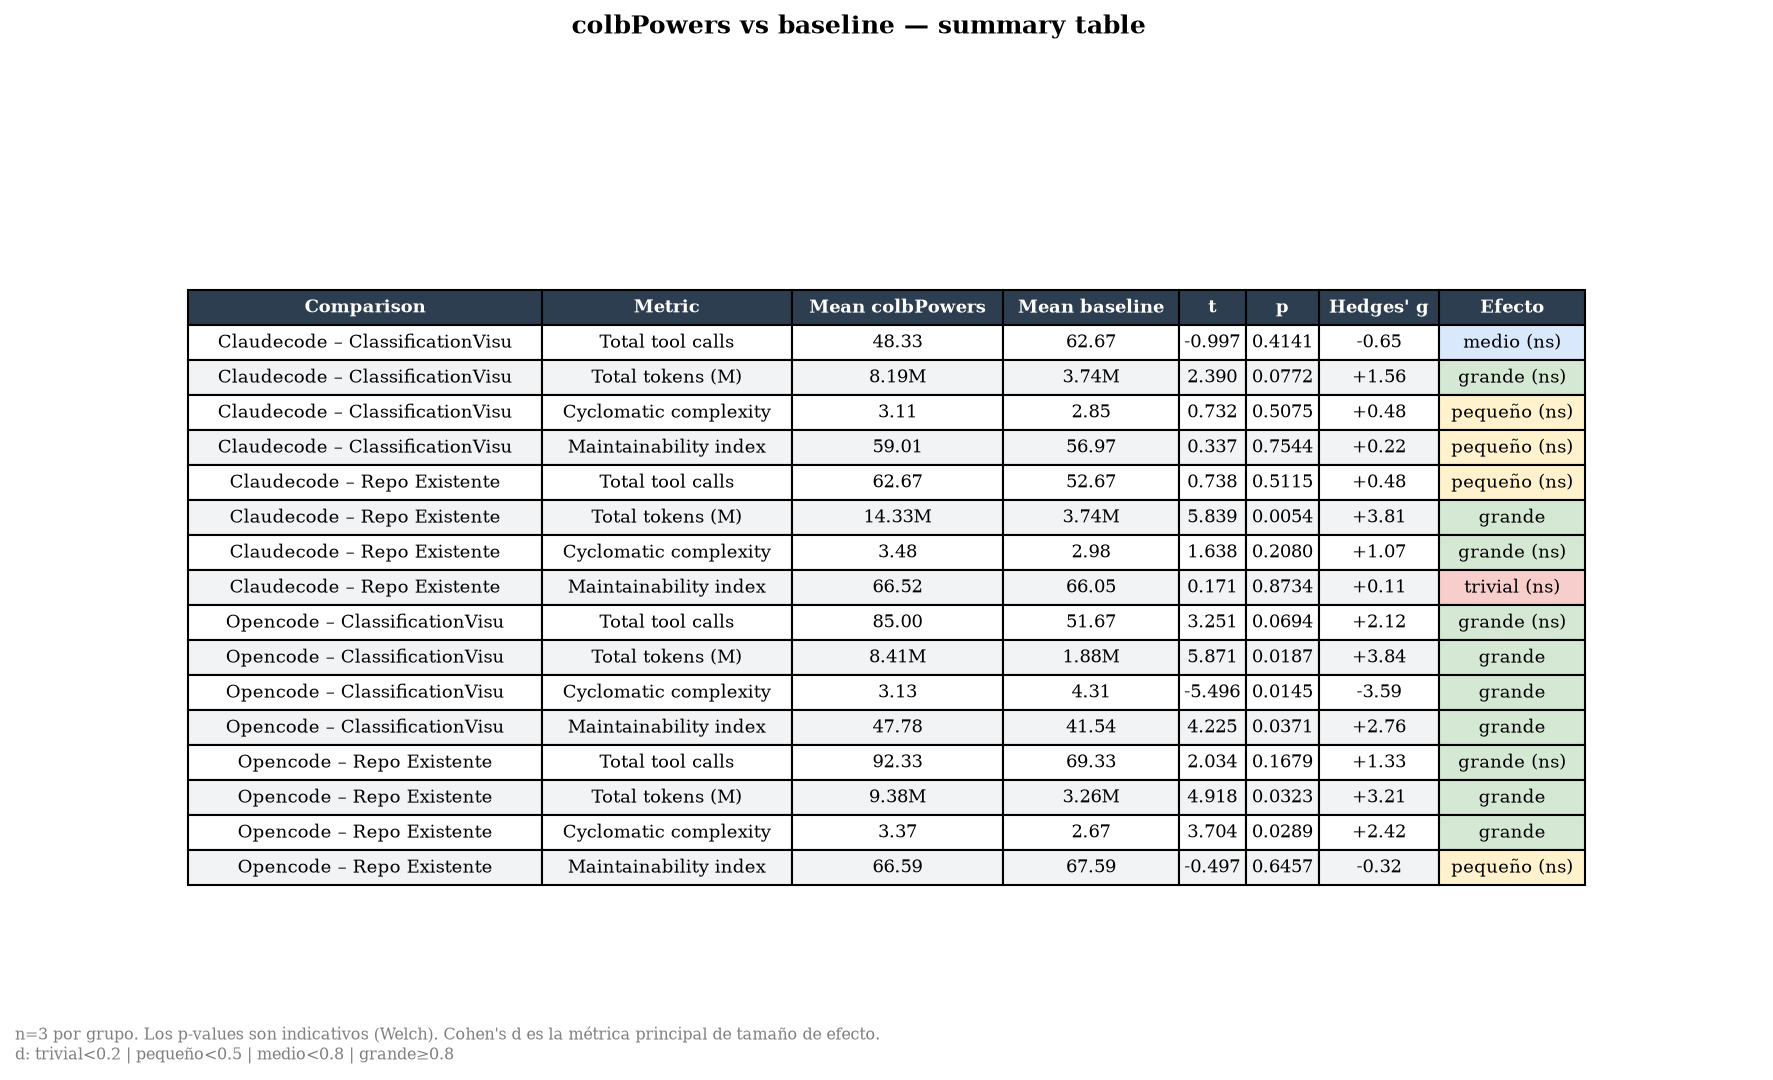
\includegraphics[width=\textwidth]{graficos/ttest_analisis/results_cpbl_table.png}
    \caption{Análisis estadístico completo: colbPowers vs.\ baseline. Se incluye la $d$ de Cohen como métrica principal del tamaño de efecto.}
    \label{fig:ttest_cpbl}
\end{figure}

\begin{figure}[H]
    \centering
    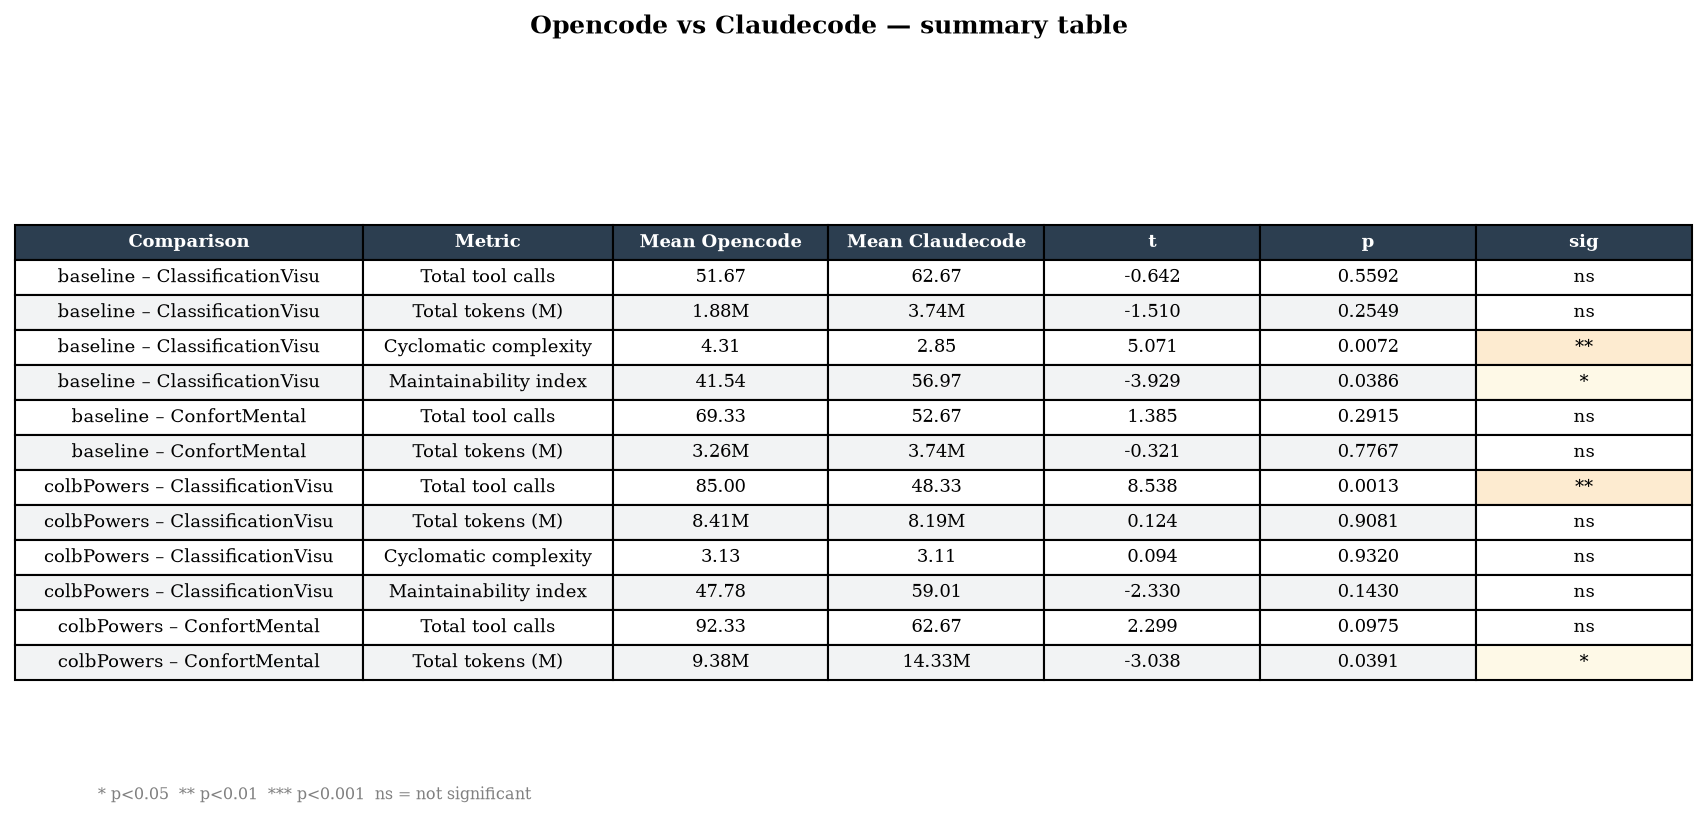
\includegraphics[width=\textwidth]{graficos/ttest_analisis/results_occc_table.png}
    \caption{Análisis estadístico completo: OpenCode vs.\ ClaudeCode. Se incluye la $d$ de Cohen como métrica principal del tamaño de efecto.}
    \label{fig:ttest_occc}
\end{figure}

\section{Gráficas adicionales del experimento}
\label{sec:anexo_graficas}

\begin{figure}[H]
    \centering
    
\includegraphics[width=\textwidth]{graficos/comparisons/03_desglose_tokens.png}
    \caption{Desglose de tokens por tipo (input, output, caché leída) para cada experimento y condición.}
    \label{fig:desglose_tokens}
\end{figure}

\begin{figure}[H]
    \centering
    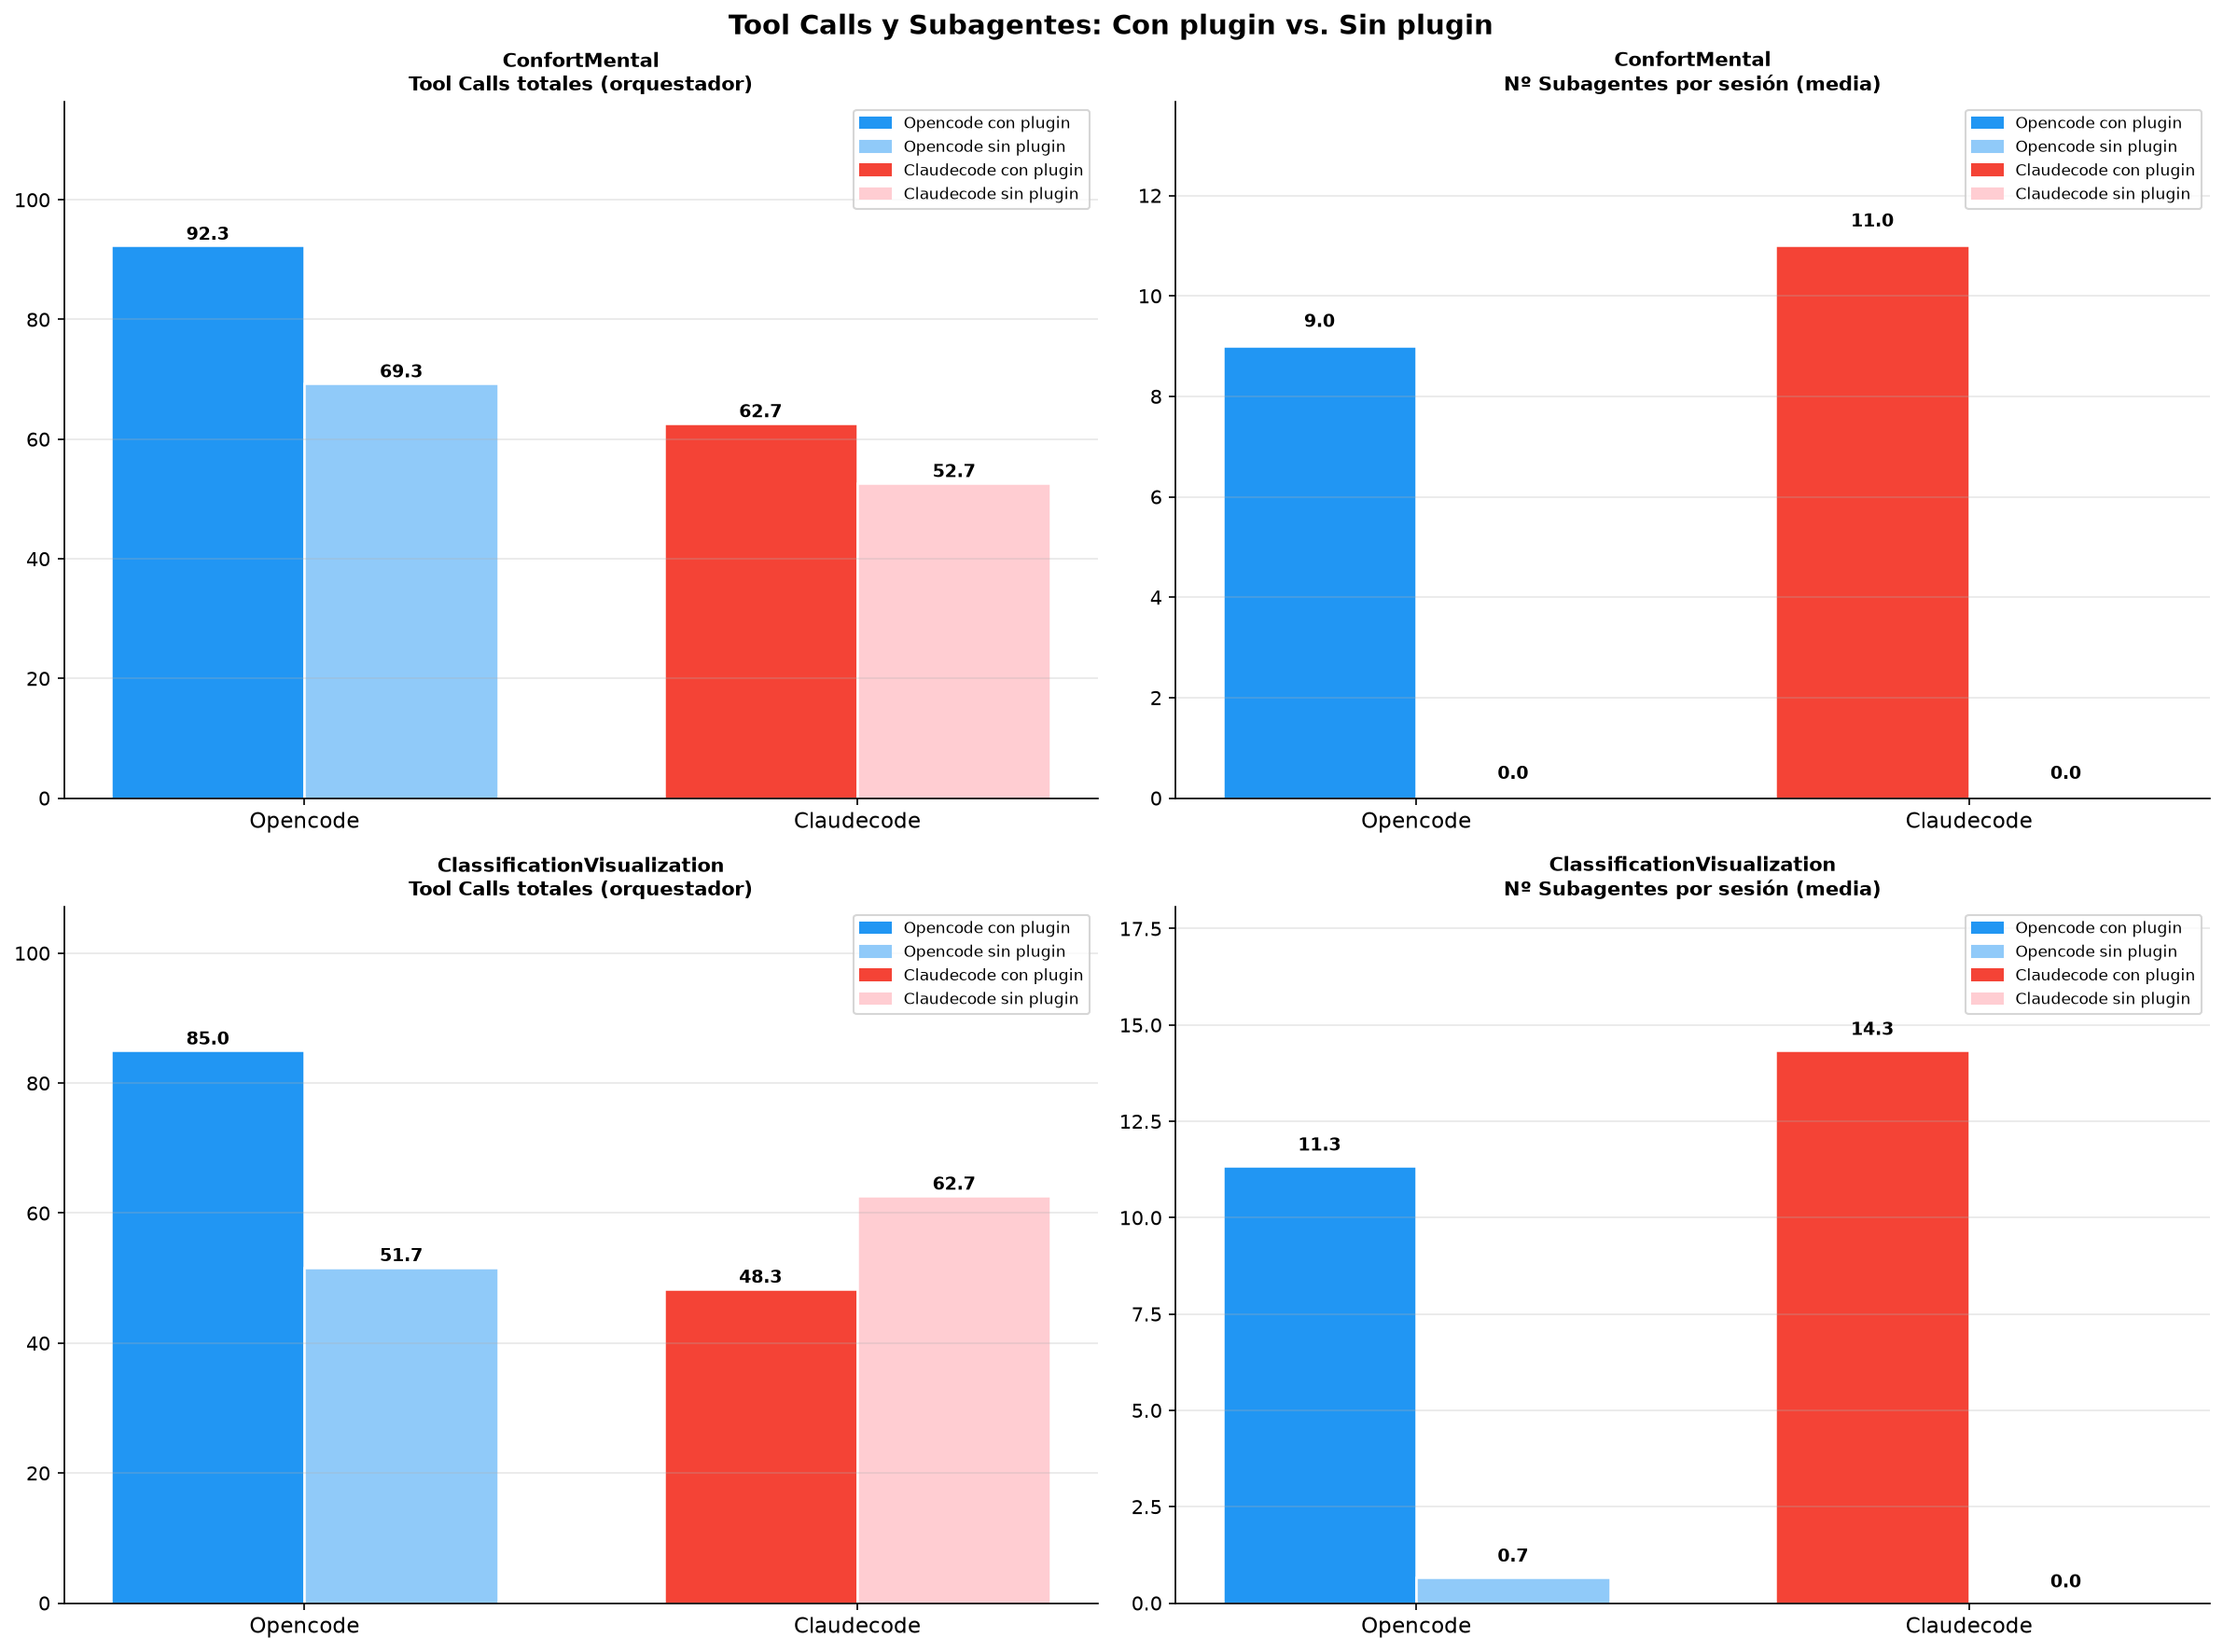
\includegraphics[width=\textwidth]{graficos/comparisons/04_toolcalls_subagentes.png}
    \caption{Tool calls totales del orquestador y número de subagentes por sesión, por condición y experimento.}
    \label{fig:toolcalls_subagentes}
\end{figure}

\begin{figure}[H]
    \centering
    
\includegraphics[width=\textwidth]{graficos/comparisons/05_crg_llamadas.png}
    \caption{Llamadas al plugin code-review-graph por condición y experimento.}
    \label{fig:crg_llamadas}
\end{figure}

\begin{figure}[H]
    \centering
    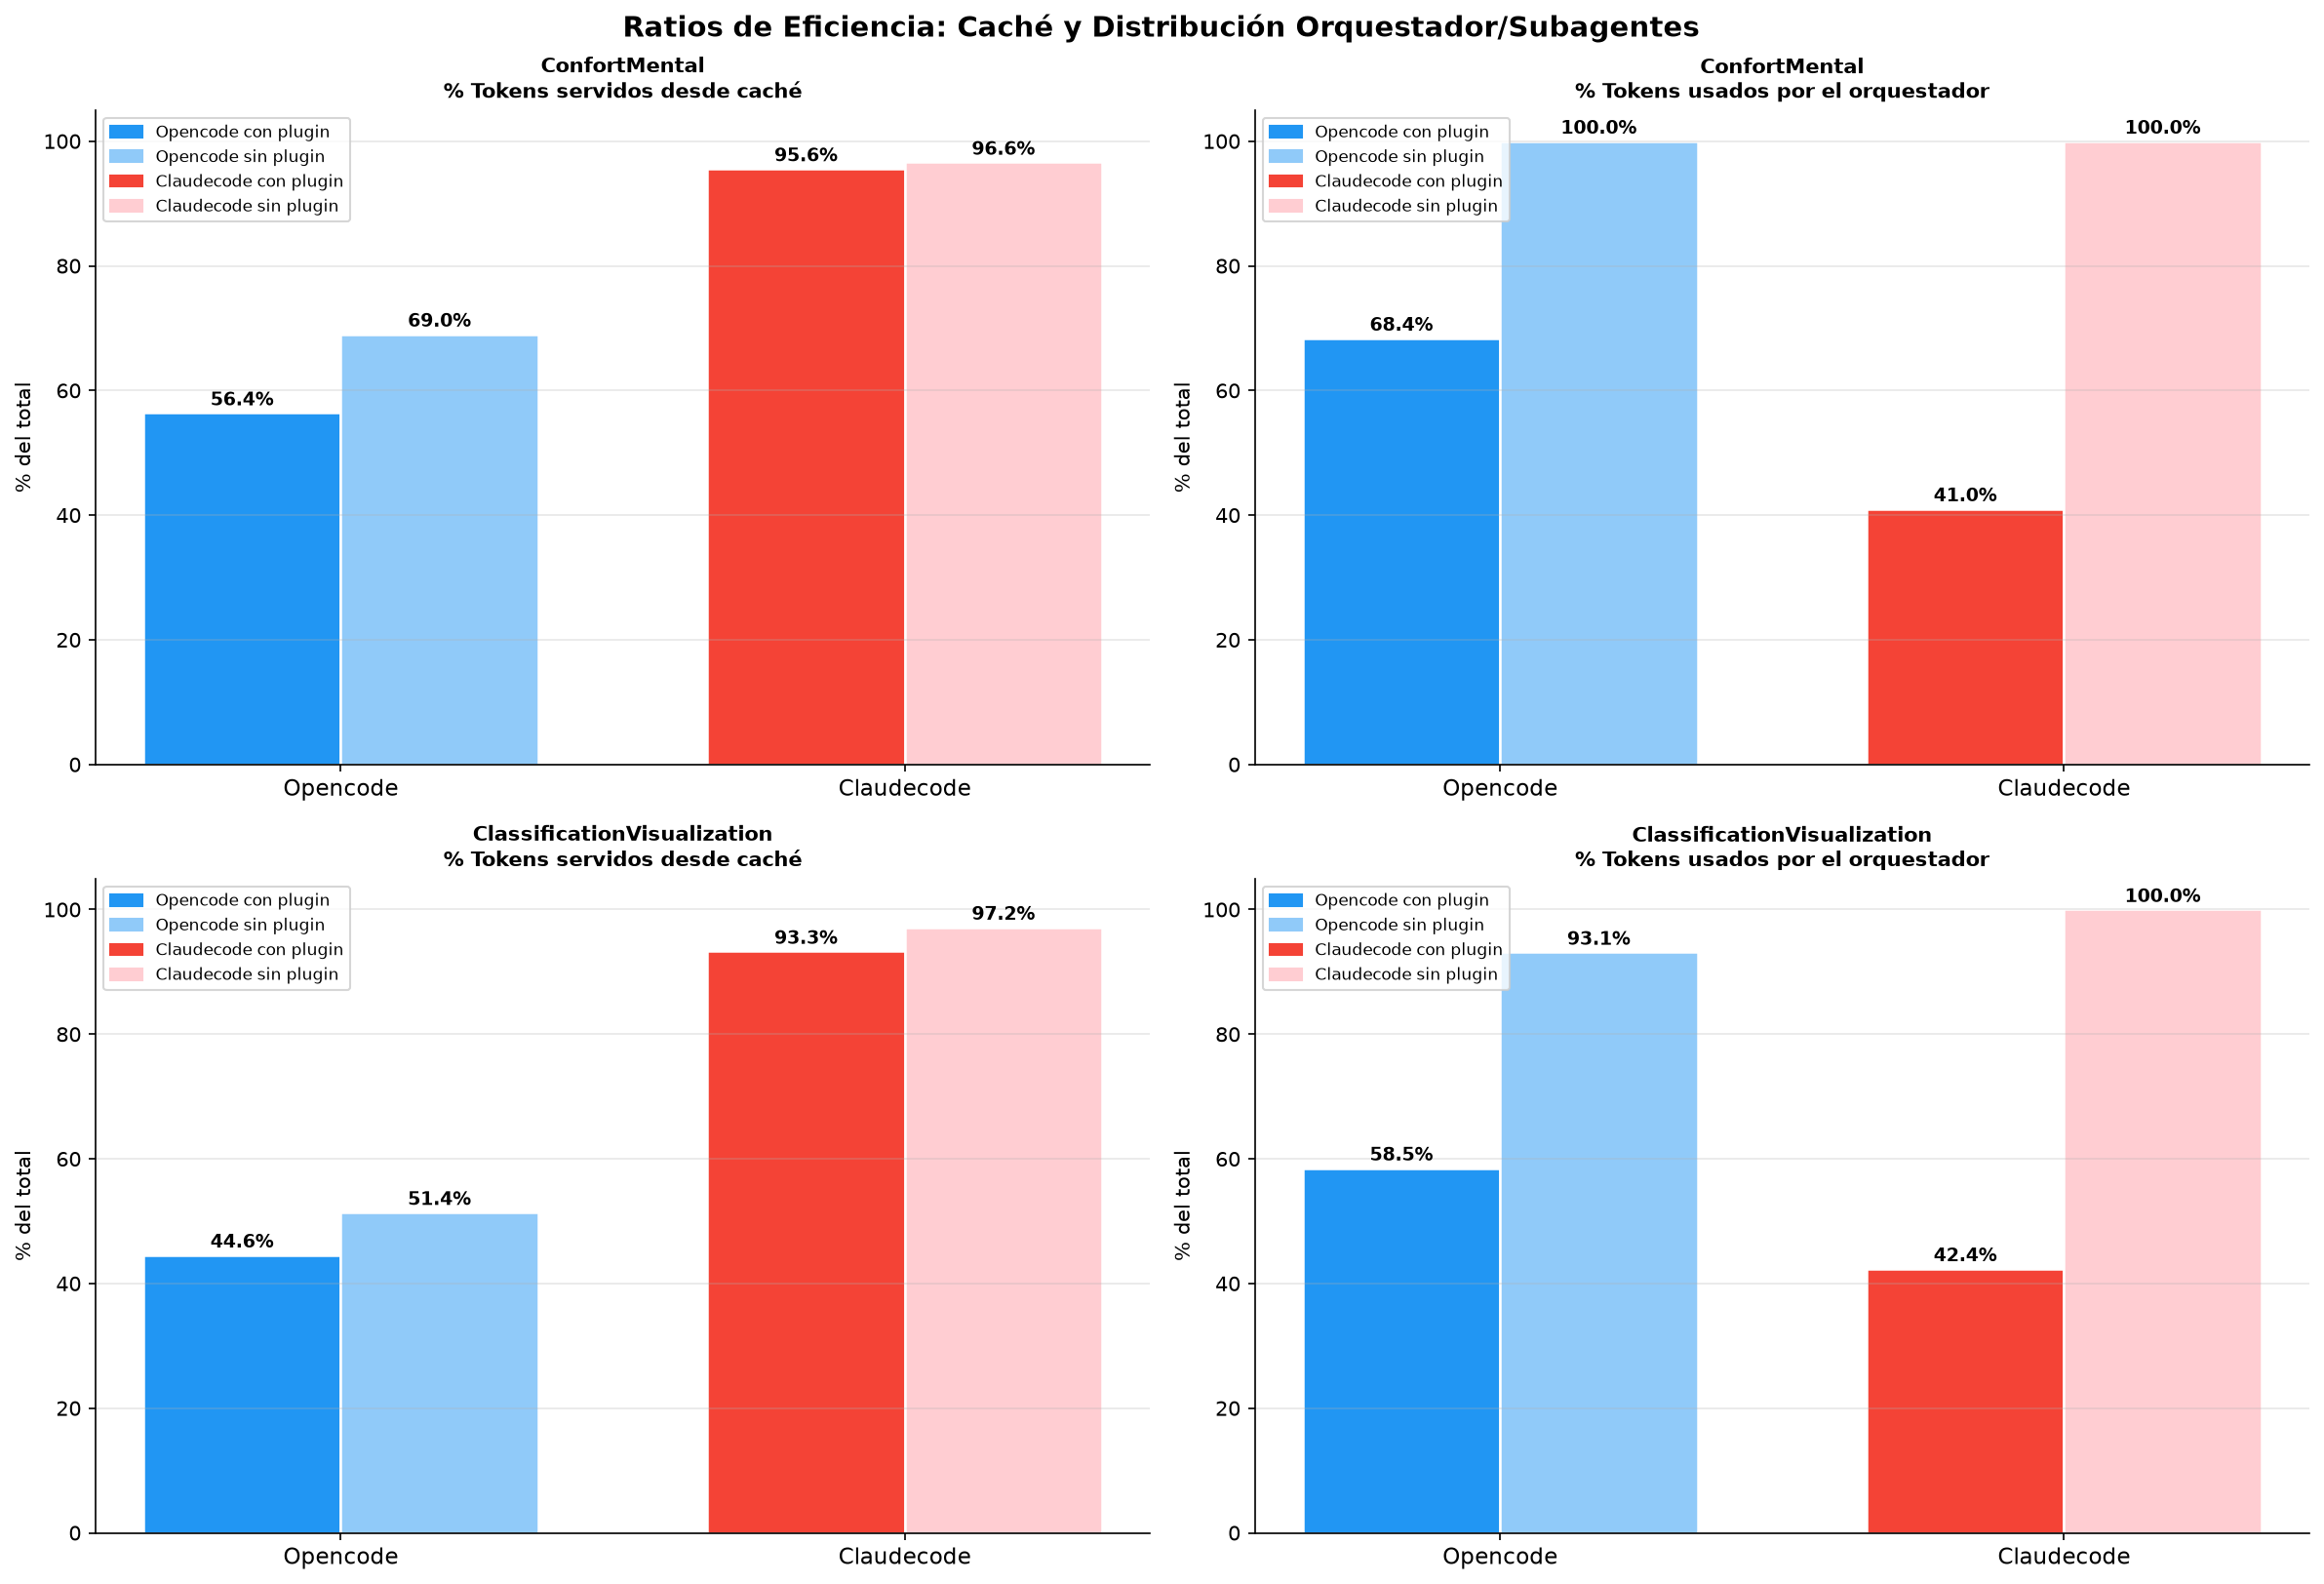
\includegraphics[width=\textwidth]{graficos/comparisons/06_ratios_eficiencia.png}
    \caption{Ratios de eficiencia: porcentaje de tokens servidos desde caché y porcentaje de tokens consumidos por el orquestador.}
    \label{fig:ratios_eficiencia}
\end{figure}

\begin{figure}[H]
    \centering
    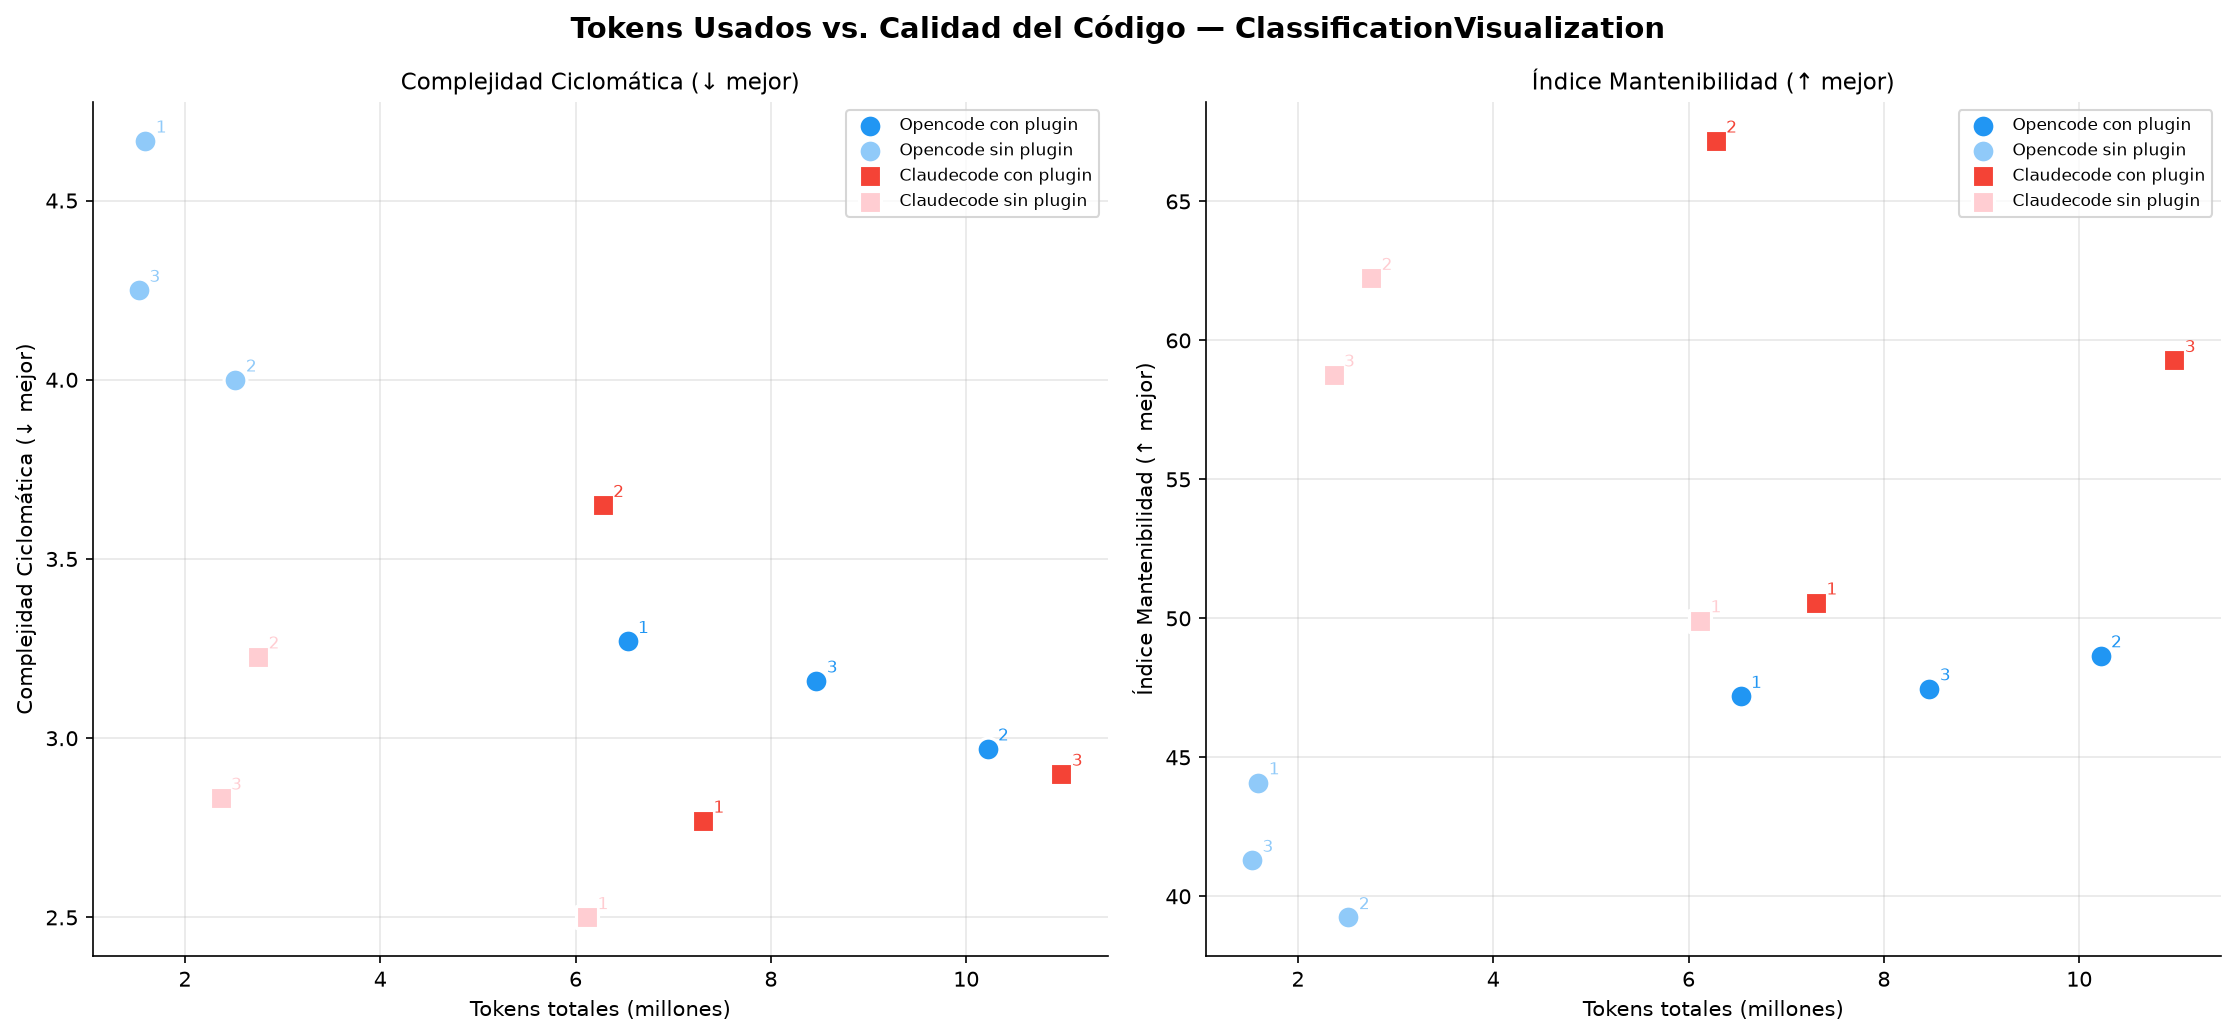
\includegraphics[width=\textwidth]{graficos/comparisons/07_tokens_vs_calidad.png}
    \caption{Dispersión: tokens totales vs.\ métricas de calidad del código (Caso~2). Cada punto representa una sesión individual.}
    \label{fig:tokens_vs_calidad}
\end{figure}

\begin{figure}[H]
    \centering
    
\includegraphics[width=\textwidth]{graficos/comparisons/09_distribucion_toolcalls.png}
    \caption{Distribución de tool calls del orquestador por tipo (top~10 herramientas, sesiones con colbPowers).}
    \label{fig:distribucion_toolcalls}
\end{figure}

\end{document}